% ******************************* PhD Thesis Template **************************
% Please have a look at the README.md file for info on how to use the template

\documentclass[a4paper,11pt,numbered,draft,pdftex,dvipsnames]{Classes/PhDThesisPSnPDF}

% ******************************************************************************
% ******************************* Class Options ********************************
% *********************** See README for more details **************************
% ******************************************************************************

% `a4paper'(The University of Cambridge PhD thesis guidelines recommends a page
% size a4 - default option) or `a5paper': A5 Paper size is also allowed as per
% the Cambridge University Engineering Department guidelines for PhD thesis
%
% `11pt' or `12pt'(default): Font Size 10pt is NOT recommended by the University
% guidelines
%
% `oneside' or `twoside'(default): Printing double side (twoside) or single
% side.
%
% `print': Use `print' for print version with appropriate margins and page
% layout. Leaving the options field blank will activate Online version.
%
% `index': For index at the end of the thesis
%
% `draftclassic': For draft mode without loading any images (same as draft in book)
%
% `draft': Special draft mode with line numbers, images, and water mark with
% timestamp and custom text. Position of the text can also be modified.
%
% `abstract': To generate only the title page and abstract page with
% dissertation title and name, to submit to the Student Registry
%
% `chapter`: This option enables only the specified chapter and it's references
%  Useful for review and corrections.
%
% ************************* Custom Page Margins ********************************
%
% `custommargin`: Use `custommargin' in options to activate custom page margins,
% which can be defined in the preamble.tex. Custom margin will override
% print/online margin setup.
%
% *********************** Choosing the Fonts in Class Options ******************
%
% `times' : Times font with math support. (The Cambridge University guidelines
% recommend using times)
%
% `fourier': Utopia Font with Fourier Math font (Font has to be installed)
%            It's a free font.
%
% `customfont': Use `customfont' option in the document class and load the
% package in the preamble.tex
%
% default or leave empty: `Latin Modern' font will be loaded.
%
% ********************** Choosing the Bibliography style ***********************
%
% `authoryear': For author-year citation eg., Krishna (2013)
%
% `numbered': (Default Option) For numbered and sorted citation e.g., [1,5,2]
%
% `custombib': Define your own bibliography style in the `preamble.tex' file.
%              `\RequirePackage[square, sort, numbers, authoryear]{natbib}'.
%              This can be also used to load biblatex instead of natbib
%              (See Preamble)
%
% **************************** Choosing the Page Style *************************
%
% `default (leave empty)': For Page Numbers in Header (Left Even, Right Odd) and
% Chapter Name in Header (Right Even) and Section Name (Left Odd). Blank Footer.
%
% `PageStyleI': Chapter Name next & Page Number on Even Side (Left Even).
% Section Name & Page Number in Header on Odd Side (Right Odd). Footer is empty.
%
% `PageStyleII': Chapter Name on Even Side (Left Even) in Header. Section Number
% and Section Name in Header on Odd Side (Right Odd). Page numbering in footer

% Uncomment to change page style
%\pagestyle{PageStyleII}

% ********************************** Preamble **********************************
% Preamble: Contains packages and user-defined commands and settings
% ******************************************************************************
% ****************************** Custom Margin *********************************

% Add `custommargin' in the document class options to use this section
% Set {innerside margin / outerside margin / topmargin / bottom margin}  and
% other page dimensions
\ifsetCustomMargin
  \RequirePackage[left=25mm,right=25mm,top=25mm,bottom=25mm]{geometry}
  \setFancyHdr % To apply fancy header after geometry package is loaded
\fi

% Add spaces between paragraphs
\setlength{\parskip}{0.5em}
%Set indentation length for paragraphs
\setlength{\parindent}{0pt}
% Ragged bottom avoids extra whitespaces between paragraphs
\raggedbottom
% To remove the excess top spacing for enumeration, list and description
%\usepackage{enumitem}
%\setlist[enumerate,itemize,description]{topsep=0em}

% *****************************************************************************
% ******************* Fonts (like different typewriter fonts etc.)*************

% Add `customfont' in the document class option to use this section

\usepackage{sectsty} % for sf sections
\allsectionsfont{\sffamily} % all sections in sans-serif font
	
%
\ifsetCustomFont

  \usepackage[tt=false]{libertinus}
  \usepackage[
  	libertine,
  	upint,
  	slantedGreek
  ]{newtxmath}
  \usepackage[zerostyle=d,scaled=.94]{newtxtt}
  
  \AtBeginDocument{%
  \DeclareMathSymbol{0}{\mathalpha}{operators}{`0}%
  \DeclareMathSymbol{1}{\mathalpha}{operators}{`1}%
  \DeclareMathSymbol{2}{\mathalpha}{operators}{`2}%
  \DeclareMathSymbol{3}{\mathalpha}{operators}{`3}%
  \DeclareMathSymbol{4}{\mathalpha}{operators}{`4}%
  \DeclareMathSymbol{5}{\mathalpha}{operators}{`5}%
  \DeclareMathSymbol{6}{\mathalpha}{operators}{`6}%
  \DeclareMathSymbol{7}{\mathalpha}{operators}{`7}%
  \DeclareMathSymbol{8}{\mathalpha}{operators}{`8}%
  \DeclareMathSymbol{9}{\mathalpha}{operators}{`9}%
  }
  
  \DeclareMathAlphabet{\mathcal}{OMS}{cmsy}{m}{n} % get me my nice mathcals back
\fi

% *****************************************************************************
% **************************** Custom Packages ********************************

% ************************* Algorithms and Pseudocode **************************

%\usepackage{algpseudocode}


% ********************Captions and Hyperreferencing / URL **********************

% Captions: This makes captions of figures use a boldfaced small font.
%\RequirePackage[small,bf]{caption}

\RequirePackage[small,tableposition=top,labelfont=bf]{caption}
%\renewcommand{\figurename}{Figure~} %to support older versions of captions.sty
%\renewcommand{\tablename}{Table~}

% *************************** Graphics and figures *****************************

%\usepackage{rotating}
%\usepackage{wrapfig}

% Uncomment the following two lines to force Latex to place the figure.
% Use [H] when including graphics. Note 'H' instead of 'h'
%\usepackage{float}
%\restylefloat{figure}
\renewcommand{\topfraction}{.75}
% Subcaption package is also available in the sty folder you can use that by
% uncommenting the following line
% This is for people stuck with older versions of texlive
%\usepackage{sty/caption/subcaption}
\usepackage[labelformat=simple]{subcaption}
\renewcommand\thesubfigure{(\alph{subfigure})}
%
%\DeclareSubrefFormat{myparens}{#1~(#2)}
%\captionsetup[subfloat]{subrefformat=myparens}

% ********************************** Tables ************************************
\usepackage{booktabs} % For professional looking tables
\usepackage{multirow}

\usepackage{multicol}
%\usepackage{longtable}
%\usepackage{tabularx}
\usepackage{etoolbox}
\AtBeginEnvironment{tabular}{\small}


% *********************************** SI Units *********************************
\usepackage[binary-units=true,mode=text]{siunitx} % use this package module for SI units


% ******************************* Line Spacing *********************************

% Choose linespacing as appropriate. Default is one-half line spacing as per the
% University guidelines

% \doublespacing
% \onehalfspacing
\singlespacing
\frenchspacing

% ******************************* Language *********************************
\ifxetex
  	\usepackage{polyglossia}
\else
	\usepackage[ngerman,british]{babel}
\fi
% ******************************** Hyphenations**********************************

\ifxetex
	\tolerance=1
	\emergencystretch=\maxdimen
	\hyphenpenalty=10000
	\hbadness=10000
\else
	\hyphenchar\font=\string"7F
	%\hyphenation{Trans-zen-denz trans-zen-dent}

	\begin{hyphenrules}{ngerman}
		\hyphenation{Arbeits-at-mo-sphä-re}
	\end{hyphenrules}
\fi
% ************************ Formatting / Footnote *******************************

% Don't break enumeration (etc.) across pages in an ugly manner (default 10000)
%\clubpenalty=500
%\widowpenalty=500
\usepackage{footnotebackref}
\usepackage[perpage,hang,symbol]{footmisc} %Range of footnote options
%\renewcommand*{\thefootnote}{(\arabic{footnote})}
\DefineFNsymbols*{lamportnostar}[math]{\dagger\S\ddagger\P\|{\dagger\dagger}{\ddagger\ddagger}}
\setfnsymbol{lamportnostar}
% *****************************************************************************
% *************************** Bibliography  and References ********************

\usepackage{cleveref} %Referencing without need to explicitly state fig /table

% Add `custombib' in the document class option to use this section
\ifuseCustomBib
   \RequirePackage[square, sort, numbers, authoryear]{natbib} % CustomBib

% If you would like to use biblatex for your reference management, as opposed to the default `natbibpackage` pass the option `custombib` in the document class. Comment out the previous line to make sure you don't load the natbib package. Uncomment the following lines and specify the location of references.bib file

%\RequirePackage[backend=biber, style=numeric, citestyle=numeric, natbib=true, sorting=none]{biblatex}
%%\addbibresource{References/dummy.bib}
%\addbibresource{References/references.bib}
%\addbibresource{References/atlas_journal.bib}
%\addbibresource{References/atlas_pub.bib}
%\addbibresource{References/atlas_conf.bib}
%\addbibresource{References/websites.bib} %Location of references.bib only for biblatex, Do not omit the .bib extension from the filename.

\fi

% changes the default name `Bibliography` -> `References'
\renewcommand{\bibname}{References}


% ******************************************************************************
% ************************* User Defined Commands ******************************
% ******************************************************************************

% *********** To change the name of Table of Contents / LOF and LOT ************

%\renewcommand{\contentsname}{My Table of Contents}
%\renewcommand{\listfigurename}{My List of Figures}
%\renewcommand{\listtablename}{My List of Tables}

% ********************** Make broken labels extra visible *************************

\makeatletter
\patchcmd{\@setref}{\bfseries ??}{\bfseries\color{red} undefined Label}{}{}

% ********************** TOC depth and numbering depth *************************

\setcounter{secnumdepth}{2}
\setcounter{tocdepth}{2}

\usepackage[titles]{tocloft}
\setlength{\cftbeforepartskip}{12pt}
\setlength{\cftbeforechapskip}{2pt}
\setlength{\cftbeforesecskip}{-4pt}
\setlength{\cftbeforesubsecskip}{-5pt}
%\setlength\cftparskip{-2pt}

% ******************************* Nomenclature *********************************
% To change the name of the Nomenclature section, uncomment the following line
\renewcommand{\nomname}{Symbols}

\RequirePackage[acronym]{glossaries}
\renewcommand*{\glstextformat}[1]{\textcolor{black}{#1}}
\makeglossaries

% ********************************* Appendix ***********************************

% The default value of both \appendixtocname and \appendixpagename is `Appendices'. These names can all be changed via:

%\renewcommand{\appendixtocname}{List of appendices}
%\renewcommand{\appendixname}{Appndx}

% *********************** Configure Draft Mode **********************************

% Uncomment to disable figures in `draft'
%\setkeys{Gin}{draft=true}  % set draft to false to enable figures in `draft'

% These options are active only during the draft mode
% Default text is "Draft"
%\SetDraftText{DRAFT}

% Default Watermark location is top. Location (top/bottom)
%\SetDraftWMPosition{bottom}

% Draft Version - default is v1.0
%\SetDraftVersion{v1.1}

% Draft Text grayscale value (should be between 0-black and 1-white)
% Default value is 0.75
%\SetDraftGrayScale{0.8}


% ******************************** Todo Notes **********************************
%% Uncomment the following lines to have todonotes.

%\ifsetDraft
%	\usepackage[colorinlistoftodos]{todonotes}
%	\newcommand{\mynote}[1]{\todo[author=kks32,size=\small,inline,color=green!40]{#1}}
%\else
%	\newcommand{\mynote}[1]{}
%	\newcommand{\listoftodos}{}
%\fi

% Example todo: \mynote{Hey! I have a note}

% ******************************** Listings **********************************

\usepackage{listings}
\usepackage{xcolor}
\crefname{lstlisting}{listing}{listings}
\Crefname{lstlisting}{Listing}{Listings}

\colorlet{punct}{black}
\definecolor{delim}{HTML}{000000}
\definecolor{kw_color}{HTML}{0b0273}
\definecolor{string_color}{HTML}{5184ad}
\definecolor{bool_color}{HTML}{2a7d18}
\colorlet{numb}{magenta!60!black}

\lstset{aboveskip=10pt,belowskip=5pt}
\lstdefinelanguage{json}{
    basicstyle=\footnotesize\ttfamily,
    keywords={true,false,null},
    keywordstyle=\color{bool_color}\bfseries,
    commentstyle=\color{black}, 
    stringstyle=\color{string_color}\bfseries,
    numberstyle=\scriptsize,
    stepnumber=1,
    numbersep=8pt,
    showstringspaces=false,
    breaklines=true,
    frame=lines,
%    backgroundcolor=\color{background},
%    comment=[s]{\ "}{"},
%    string=[s]{"}{"},
    string=[s]{"}{"},
    comment=[l]{:\ "},
    morecomment=[l]{:"},
%    morecomment=[l]{:"},
    literate=
     *{0}{{{\color{numb}0}}}{1}
      {1}{{{\color{numb}1}}}{1}
      {2}{{{\color{numb}2}}}{1}
      {3}{{{\color{numb}3}}}{1}
      {4}{{{\color{numb}4}}}{1}
      {5}{{{\color{numb}5}}}{1}
      {6}{{{\color{numb}6}}}{1}
      {7}{{{\color{numb}7}}}{1}
      {8}{{{\color{numb}8}}}{1}
      {9}{{{\color{numb}9}}}{1}
%      {:}{{{\color{punct}{:}}}}{1}
%      {,}{{{\color{punct}{,}}}}{1}
%      {\{}{{{\color{delim}{\{}}}}{1}
%      {\}}{{{\color{delim}{\}}}}}{1}
%      {[}{{{\color{delim}{[}}}}{1}
%      {]}{{{\color{delim}{]}}}}{1},
}




\usepackage{enumitem} % better enumeration
\usepackage{relsize} % for Cpp command
\usepackage{placeins}
\usepackage{braket}
%\usepackage{bbold}
\usepackage{multirow}
\usepackage{tikz}
\usepackage{tikzpagenodes}
\usepackage{pdflscape}
\usepackage{xargs}    % Use more than one optional parameter in a new commands       
\usepackage{makecell}
\usepackage{rotating} % for landscape figures
\usepackage{bbold} % double stroke numbers


% package for displaying captions on weird places
\RequirePackage{floatrow}
\floatsetup[table]{capposition=above}

% Select what to do with todonotes: 
% \usepackage[disable]{todonotes} % notes not showed
\setlength{\marginparwidth}{2cm}
\usepackage[draft,textsize=small,disable]{todonotes}   % notes showed

% ******************************** Style stuff **********************************
% ************************* Some hacks of my thesis style class I am too lazy to implement correctly ****************************
%
%\usepackage{titlesec}
%\titleformat{\chapter}[display]
%	{\normalfont\LARGE}
%	{\filleft\MakeUppercase{\chaptertitlename}\hspace{0.5cm}\rlap{\resizebox{!}{1.5cm}{\thechapter}~\rule{5cm}{1.5cm}}\hspace{0.0cm}}
%  	{10pt}
%  	{\bf\LARGE\filright}
%\titlespacing*{\chapter}{0pt}{30pt}{20pt}

%\newcommand*\HUGE{\Huge}
%\newcommand*\chapnamefont{\normalfont\LARGE\MakeUppercase}
%\newcommand*\chapnumfont{\normalfont\HUGE}
%\newcommand*\chaptitlefont{\normalfont\HUGE\bfseries}
%
%\newlength\beforechapskip
%\newlength\midchapskip
%\setlength\midchapskip{\paperwidth}
%\addtolength\midchapskip{-\textwidth}
%\addtolength\midchapskip{-\oddsidemargin}
%\addtolength\midchapskip{-1in}
%\setlength\beforechapskip{18mm}
%
%\titleformat{\chapter}[display]
%  {\normalfont\filleft}
%{{\chapnamefont\chaptertitlename}%
%\rlap{\hspace{.8em}
%\makebox[\dimexpr\paperwidth-\evensidemargin-\hoffset-1in][r]{{\resizebox{!}{\beforechapskip}{\chapnumfont\thechapter}}\quad%
%\rule{46pt}{\beforechapskip}}%
%}}%
%  {25pt}
%  {\chaptitlefont}
%\titlespacing*{\chapter}
%  {0pt}{40pt}{40pt}


% ******************************** New custom commands **********************************

\newcommand{\makemebold}[1]{%
    \ifpdf
    	\boldsymbol{#1}
    \else
    	\symbf{#1}
    \fi
}%

\newcommand{\comment}[1]
{\par {\bfseries \color{blue} #1 \par}} %comment showed
\newcommandx{\unsure}[2][1=]{\todo[linecolor=red,backgroundcolor=red!25,bordercolor=red,#1]{#2}}
\newcommandx{\change}[2][1=]{\todo[linecolor=blue,backgroundcolor=blue!25,bordercolor=blue,#1]{#2}}
\newcommandx{\info}[2][1=]{\todo[linecolor=OliveGreen,backgroundcolor=OliveGreen!25,bordercolor=OliveGreen,#1]{#2}}
\newcommandx{\improvement}[2][1=]{\todo[linecolor=Plum,backgroundcolor=Plum!25,bordercolor=Plum,#1]{#2}}
\newcommandx{\thiswillnotshow}[2][1=]{\todo[disable,#1]{#2}}

%some shortcuts for variables and symbols
\newcommand*\diff{\mathop{}\!\mathrm{d}}
\newcommand*\Diff[1]{\mathop{}\!\mathrm{d^#1}}
\newcommand*\codiff{\mathop{}\!D}
\newcommand{\Lagr}{\mathcal{L}}
\newcommand{\etmiss}{E_{\textrm{T}}^{\textrm{miss}}}
\newcommand{\met}{E_{\textrm{T}}^{\textrm{miss}}}
\newcommand{\vetmiss}{\makemebold{E}_{\textrm{T}}^{\textrm{miss}}}
\newcommand{\ptmiss}{p_{\mathrm{T}}^{\textrm{miss}}}
\newcommand{\pt}{p_{\mathrm{T}}}
\newcommand{\mbb}{m_{b\hspace{-0.06em}\bar{b}}}
\newcommand{\ptl}{p^\ell_{\textrm{T}}}
\newcommand{\mt}{m_{\textrm{T}}}
\newcommand{\mct}{m_{\textrm{CT}}}
\newcommand{\mlb}{m_{\ell b_{1}}}
\newcommand{\mjj}{m_{\textrm{jj}}}
\newcommand{\GeV}{\SI{}{\GeV}}
\newcommand{\vptlep}{\makemebold{p}_{\textrm{T}}^\ell}
\newcommand{\lsp}{\tilde{\chi}_1^0}
\newcommand{\charg}{\tilde{\chi}_1^\pm}
\newcommand{\neutr}{\tilde{\chi}_2^0}
\newcommand{\wjets}{W+\mathrm{jets}}
\newcommand{\ttbar}{t\bar{t}}


\newcommand{\onelepton}{\ensuremath{1\ell}\@\xspace}
\newcommand{\onethirtynineifb}{\ensuremath{\SI{139}{\femto\barn^{-1}}}\@\xspace}
\newcommand{\onefortyifb}{\ensuremath{\SI{140}{\femto\barn^{-1}}}\@\xspace}
\newcommand{\onefiftyifb}{\ensuremath{\SI{150}{\femto\barn^{-1}}}\@\xspace}
\newcommand{\thirtysixifb}{\ensuremath{\SI{36.1}{\femto\barn^{-1}}}\@\xspace}


\newcommand{\Rplus}{\protect\hspace{-.1em}\protect\raisebox{.15ex}{{+}}}
\newcommand{\Cpp}{\mbox{C\Rplus\Rplus}\xspace}

\newcommand{\pylib}[1]{\textsc{#1}}
\newcommand{\lib}[1]{\textsc{#1}}

%some shortcuts for common things that I need to write quite often
\newcommand{\citeneed}{\textbf{[CITATION~NEEDED]}}
\usepackage{xspace}
\newcommand*{\eg}{e.g.\@\xspace}
\newcommand*{\ie}{i.e.\@\xspace}

\makeatletter
\newcommand*{\etc}{%
	\@ifnextchar{.}%
	{etc}%
	{etc.\@\xspace}%
}
\makeatother
%these are todo notes
\newcommand\myworries[1]{\textbf{\textcolor{red}{#1}}}

% harmonise the size of single figures
\newcommand{\singlefigsize}{0.6}
\newcommand{\figname}{fig.\@\xspace}
\newcommand{\fignames}{figs.\@\xspace}
\newcommand{\Figname}{Figure}
\newcommand{\Fignames}{Figures}
\newcommand{\reference}{Ref.\@\xspace}
\newcommand{\Reference}{Ref.\@\xspace}
\newcommand{\references}{Refs.\@\xspace}
\newcommand{\References}{Refs.\@\xspace}


\newcommand{\iu}{\mathrm{i}\mkern1mu}
\newcommand{\di}{\mathrm{i}}

% ******************************** Acronyms **********************************


\newacronym{sm}{SM}{Standard Model}
\newacronym{ewk}{EWK}{electroweak}
\newacronym{hep}{HEP}{high energy physics}
\newacronym{lo}{LO}{leading order}
\newacronym[plural=HPCs,longplural={high-performance computers}]{hpc}{HPC}{high-performance computer}
\newacronym{nlo}{NLO}{next-to-leading order}
\newacronym{nll}{NLL}{next-to-leading logarithm}
\newacronym{nnlo}{NNLO}{next-to-next-to-leading order}
\newacronym{qed}{QED}{quantum electrodynamics}
\newacronym[plural=QFTs,longplural={quantum field theories}]{qft}{QFT}{quantum field theory}
\newacronym{qcd}{QCD}{quantum chromodynamics}
\newacronym[plural=VEVs,longplural={vacuum expectation values}]{vev}{VEV}{vacuum expectation value}
\newacronym{ckm}{CKM}{Cabibbo--Kobayashi--Maskawa}
\newacronym{pmns}{PMNS}{Pontecorvo--Maki--Nakagawa--Sakata}
\newacronym{susy}{SUSY}{Supersymmetry}
\newacronym{lsp}{LSP}{lightest supersymmetric particle}
\newacronym[plural=WIMPs,longplural={weakly interacting massive particles}]{wimp}{WIMP}{weakly interacting massive particle}
\newacronym{bsm}{BSM}{beyond the Standard Model}
\newacronym{cmb}{CMB}{cosmic microwave background}
\newacronym{dm}{DM}{dark matter}
\newacronym{gut}{GUT}{grand unified theory}
\newacronym{mssm}{MSSM}{Minimal Supersymmetric Standard Model}
\newacronym{pmssm}{pMSSM}{phenomenological Minimal Supersymmetric Standard Model}
\newacronym{lcdm}{$\Lambda$CDM}{Lambda Cold Dark Matter}
\newacronym{em}{EM}{Electromagnetic}
\newacronym{emec}{EMEC}{electromagnetic end-cap calorimeter}
\newacronym{hec}{HEC}{hadronic end-cap calorimeter}
\newacronym{lhc}{LHC}{Large Hadron Collider}
\newacronym{hl-lhc}{HL-LHC}{High Luminosity LHC}
\newacronym{lep}{LEP}{Large Electron Positron}
\newacronym[plural=FCNCs,longplural={flavour-changing neutral currents}]{fcnc}{FCNC}{flavour-changing neutral current}
\newacronym{rf}{RF}{radio frequency}
\newacronym{vdm}{vdM}{van der Meer}
%\newacronym{ps}{PS}{Proton Synchrotron}
%\newacronym{sps}{SPS}{Super Proton Synchrotron}
\newacronym{id}{ID}{inner detector}
\newacronym{ip}{IP}{interaction point}
\newacronym{sct}{SCT}{silicon microstip tracker}
\newacronym{trt}{TRT}{transition radiation tracker}
\newacronym{ibl}{IBL}{insertable B-layer}
\newacronym{ecal}{ECal}{electromagnetic calorimeter}
\newacronym{fcal}{FCal}{forward calorimeter}
\newacronym{hcal}{HCal}{hadronic calorimeter}
\newacronym{lar}{LAr}{liquid argon}
\newacronym{ms}{MS}{muon spectrometer}
\newacronym[plural=MDTs,longplural={Monitored Drift Tubes}]{mdt}{MDT}{Monitored Drift Tube}
\newacronym[plural=CSCs,longplural={Cathode Strip Chambers}]{csc}{CSC}{Cathode Strip Chamber}
\newacronym[plural=RPCs,longplural={Resistive Plate Chambers}]{rpc}{RPC}{Resistive Plate Chamber}
\newacronym[plural=TGCs,longplural={Thin Gap Chambers}]{tgc}{TGC}{Thin Gap Chamber}
\newacronym{zdc}{ZDC}{Zero-Degree Calorimeter}
\newacronym{alfa}{ALFA}{Absolute Luminosity for ATLAS}
\newacronym{afp}{AFP}{ATLAS Forward Proton}
\newacronym{l1}{L1}{Level~1}
\newacronym{l1topo}{L1Topo}{Level-1 Topological Processor}
\newacronym{hlt}{HLT}{High Level Trigger}
\newacronym{daq}{DAQ}{Data Acquisition System}
\newacronym[plural=ROIs,longplural={regions of interest}]{roi}{ROI}{region of interest}
\newacronym{mc}{MC}{Monte Carlo}
\newacronym{me}{ME}{matrix element}
\newacronym{ps}{PS}{parton shower}
\newacronym{isr}{ISR}{initial state radiation}
\newacronym{fsr}{FSR}{final state radiation}
\newacronym[plural=pdfs,longplural={probability density functions}]{pdf}{pdf}{probability density function}
\newacronym[plural=PDFs,longplural={parton distribution functions}]{PDF}{PDF}{parton distribution function}
\newacronym{poi}{POI}{Parameter of Interest}
\newacronym{mle}{MLE}{maximum likelihood estimator}
\newacronym{cmle}{CMLE}{conditional maximum likelihood estimator}
\newacronym{hf}{HF}{heavy flavour}
\newacronym{vbf}{VBF}{vector boson fusion}
\newacronym{ggf}{ggF}{gluon--gluon fusion}
\newacronym{jes}{JES}{jet energy scale}
\newacronym{jer}{JER}{jet energy resolution}
\newacronym{jvt}{JVT}{jet vertex tagger}
\newacronym{gsc}{GSC}{global sequential calibration}
\newacronym{bdt}{BDT}{boosted decision tree}
\newacronym{dr}{DR}{diagram removal}
\newacronym{ds}{DS}{diagram subtraction}
\newacronym{cp}{CP}{combined performance}
\newacronym{roc}{ROC}{receiver operating characteristic}
\newacronym[plural=SRs,longplural={signal regions}]{sr}{SR}{signal region}
\newacronym[plural=CRs,longplural={control regions}]{cr}{CR}{control region}
\newacronym[plural=VRs,longplural={validation regions}]{vr}{VR}{validation region}


% ************************ Thesis Information & Meta-data **********************
% Thesis title and author information, refernce file for biblatex
% ************************ Thesis Information & Meta-data **********************
%% The title of the thesis

%\newcommand{\myTitle}{Search for charginos and neutralinos in a signature with a Higgs boson and an isolated lepton with the ATLAS detector and its reinterpretation in the phenomenological MSSM}
\newcommand{\myTitle}{Search for Charginos and Neutralinos in a Signature with a Higgs Boson and an Isolated Lepton with the ATLAS Detector and its Reinterpretation in the Phenomenological MSSM}
%Search for Charginos and Neutralinos in a Signature with a Higgs Boson and an Isolated Lepton with the ATLAS Detector and Its Reinterpretation in the Phenomenological MSSM
\title{\myTitle}
%\texorpdfstring is used for PDF metadata. Usage:
%\texorpdfstring{LaTeX_Version}{PDF Version (non-latex)} eg.,
%\texorpdfstring{$sigma$}{sigma}

%% Subtitle (Optional)
%\subtitle{Neue Elemente zur Erweiterung der Suche nach Supersymmetrie in Ereignissen mit einem isolierten Lepton, Jets und fehlender transversaler Energie mit dem ATLAS Detektor}

%% The full name of the author
\author{Eric Schanet}

\location{M\"unchen}

%% Department (eg. Department of Engineering, Maths, Physics)
\dept{Dissertation an der Fakult\"at f\"ur Physik}

%% University and Crest
\university{der\\Ludwig--Maximilians--Universit\"at M\"unchen}
% Crest minimum should be 30mm.
\crest{
\includegraphics[width=0.3\textwidth]{Figs/Sigillum_Universitatis_Ludovico-Maximilianeae_interlaced}}
%% Use this crest, if you are using the college crest
%% Crest long miminum should be 65mm
%\crest{
\includegraphics[width=0.45\textwidth]{University_Crest_Long}}

%% You can redefine the submission text:
% Default as per the University guidelines:
% ``This dissertation is submitted for the degree of''
%\renewcommand{\submissiontext}{change the default text here if needed}

%% Full title of the Degree
\degreetitle{Dissertation}

%% College affiliation (optional)
%\college{}

%% Submission date
% Default is set as {\monthname[\the\month]\space\the\year}
\degreedate{M\"unchen, den 7. Mai 2021} 

%% Meta information
\subject{LaTeX} \keywords{{LaTeX} {PhD Thesis} {Particle Physics} {Supersymmetry} {Ludwig-Maximilians-University Munich}}


% ***************************** Abstract Separate ******************************
% To printout only the titlepage and the abstract with the PhD title and the
% author name for submission to the Student Registry, use the `abstract' option in
% the document class.

\ifdefineAbstract
 \pagestyle{empty}
 \includeonly{Declaration/declaration, Abstract/abstract}
\fi

% ***************************** Chapter Mode ***********************************
% The chapter mode allows user to only print particular chapters with references
% Title, Contents, Frontmatter are disabled by default
% Useful option to review a particular chapter or to send it to supervisior.
% To use choose `chapter' option in the document class

\ifdefineChapter
%	\includeonly{Introduction/introduction}
%	\includeonly{chapter-theory/theory}
%	\includeonly{chapter-experiment/experiment}
%	\includeonly{chapter-mc/mc}
%	\includeonly{chapter-1lepton/1lepton}
%	\includeonly{chapter-statistics/statistics}
%	\includeonly{chapter-electroweak/electroweak}
%	\includeonly{chapter-pmssm/pmssm}
%	\includeonly{chapter-summary/summary}
\fi

% ******************************** Front Matter ********************************
\begin{document}

\frontmatter

\maketitle

\cleardoublepage

\makegermantitle
%supervisors here
\newpage
Supervisor: Prof.\@\xspace Dr.\@\xspace Dorothee Schaile

% ************************** Thesis Abstract *****************************
% Use `abstract' as an option in the document class to print only the titlepage and the abstract.

\sisetup{output-decimal-marker = {,}}
\begin{otherlanguage}{ngerman} 
\begin{zusammenfassung}

Obwohl das Standardmodell der Teilchenphysik eine außerordentlich erfolgreiche Theorie darstellt, deuten einige Beobachtungen auf die Existenz neuer Physik jenseits dessen was im Rahmen des Standardmodells erklärt werden kann hin.
Supersymmetrie ist der Oberbegriff für eine Klasse von Theorien, die einige der offenen Fragen des Standardmodells erklären könnten.
Sie sagt die Existenz von supersymmetrischen Partnern für jedes Teilchen des Standardmodells voraus und könnte, unter anderem, einen Teilchenkandidaten für Dunkle Materie liefern. 

Diese Arbeit stellt eine Suche nach supersymmetrischen Teilchen, die über die elektroschwache Wechsel\-wirkung paarproduziert werden, vor.
Endzustände mit einem Lepton, fehlender Transversal\-energie und einem Higgs Boson, welches in zwei \textit{b}-Quarks zerfällt, werden untersucht.
Insgesamt werden \onethirtynineifb an Daten aus Proton-Proton Kollisionen berücksichtigt, welche mit dem ATLAS Detektor bei einer Schwerpunktsenergie von $\sqrt{s}=\SI{13}{\TeV}$ im Run~2 des Large Hadron Colliders aufgezeichnet wurden.
Ein, auf einer Likelihood-Methode basierender, simultaner Fit in allen Suchregionen wird verwendet, um hohe Sensitivität zu möglichst vielen kinematischen Bereichen im untersuchten Parameterraum zu gewährleisten.

In den Daten wird keine signifikante Abweichung von den Standardmodellvorhersagen beobachtet, weshalb die Ergebnisse in einem vereinfachten Modell für Paarproduktion der supersymmetrischen Partner des Higgs-Bosons und der Eichbosonen interpretiert werden.
Für leichteste Neutralinos mit Massen von $\lesssim \SI{100}{\GeV}$ ($\approx\SI{250}{\GeV}$), können leichteste Charginos und zweitleichteste Neutralinos mit Massen von bis zu $\SI{740}{\GeV}$ ($\SI{600}{\GeV}$) ausgeschlossen werden.

Da heutige Teilchenphysik-Experimente aufgrund ihrer Komplexität und Größenordnung nicht trivial reproduzierbar sind, gleichzeitig aber eine Vielzahl an Modellen für Physik jenseits des Standardmodells existiert, wird ein besonderes Augenmerk auf die technische Durchführbarkeit einer Neuinterpretation der Suche gelegt.
Die volle Likelihood-Funktion der Suche wurde veröffentlicht und eine vollständig reproduzierbare Umsetzung der Suche anhand Container-Technologie und parametrisierter Job-Vorlagen wird diskutiert.
Mit Hinblick auf rechenintensive Neuinterpretationen in hoch-dimensionalen Parameter\-räumen wird eine Methode eingeführt, um die Likelihood-Funktionen von ATLAS Suchen nach Supersymmetrie zu nähern.
Mit Hilfe dieser Methode wird schlussendlich eine Neuinterpretation der Suche in einem Unterraum einer 19-dimensionalen Menge von vollständigeren supersymmetrischen Modellen durchgeführt und deren Ergebnisse diskutiert. 

\end{zusammenfassung}
\end{otherlanguage}  
\sisetup{output-decimal-marker = {.}}

\begin{abstract}

Despite the success of the Standard Model of particle physics, a number of hints suggest the existence of new physics beyond the scope of phenomena that can be explained in the theoretical framework of the Standard Model.
One class of theories that could be able to explain some of the open questions of the Standard Model is Supersymmetry. It introduces supersymmetric partners to each of the Standard Model particles, and could, for example, provide a candidate for Dark Matter.

This thesis presents a search for electroweak production of supersymmetric particles in events with a lepton, missing transverse momentum and a Higgs boson decaying into two \textit{b}-quarks.
The search analyses \onethirtynineifb of proton--proton collision data at a centre-of-mass energy of $\sqrt{s}=\SI{13}{\TeV}$, recorded by the ATLAS detector at the Large Hadron Collider.
A likelihood-based simultaneous fit in all search regions is introduced in order to achieve sensitivity to a large variety of kinematic regimes.

No significant deviation from the Standard Model predictions is seen in data in any of the search regions.
The results are subsequently interpreted in a simplified model for pair production of the supersymmetric partners of the Higgs and gauge bosons.
Lightest chargino and next-to-lightest neutralino masses of $\SI{740}{\GeV}$ ($\SI{600}{\GeV}$) can be excluded for lightest neutralino masses of $\lesssim \SI{100}{\GeV}$ ($\approx\SI{250}{\GeV}$).
%, significantly improving the limits set by previous ATLAS searches for Supersymmetry.

Given that the particle physics experiments at the Large Hadron Collider are not easily reproducible, and a large number of phenomenologically viable models for physics beyond the Standard Model exist, special focus is put on the reusability and reinterpretability of the search.
The full likelihood function of the search is published in a readily available format, and a fully reusable implementation of the search using containerised workflows with parameterised job templates is provided. 
In light of conceptually interesting  but computationally challenging reinterpretations in high-dimensional model spaces, a method for generically approximating the likelihood functions of ATLAS searches for Supersymmetry is introduced and validated. Using this approach, a reinterpretation of the search in a subspace of a 19-dimensional set of more complete supersymmetric models is performed and its results are discussed. 

\end{abstract}




% *********************** Adding TOC and List of Figures ***********************

\tableofcontents

%\listoffigures
%
%\listoftables

% \printnomenclature[space] space can be set as 2em between symbol and description


%\printnomenclature

% ******************************** Main Matter *********************************
\mainmatter

\listoftodos[Notes]
%!TEX root = ../thesis.tex
%*******************************************************************************
%*********************************** Introduction *****************************
%*******************************************************************************

\chapter*{Introduction}
\markboth{Introduction}{}
\ifpdf
    \graphicspath{{Chapter1/Figs/Raster/}{Chapter1/Figs/PDF/}{Chapter1/Figs/}}
\else
    \graphicspath{{Chapter1/Figs/Vector/}{Chapter1/Figs/}}
\fi

Particle physics studies the fundamental constituents and interactions of matter with the ultimate goal of uncovering the laws of nature that govern the most fundamental building blocks of the universe. Over the course of more than a century, fundamental physics has continuously pushed the intellectual frontier to new realms, reaching ever-smaller length-scales on which the fundamental interactions of the building blocks of matter can be understood. The resulting theoretical framework, the \gls{sm}, provides answers to some of the deepest questions that can be asked about the universe and is the most fundamental, experimentally validated description of nature known to date. 

Particle physics finds itself, however, at an interesting crossroad. On the hand, the \gls{sm} is very successful in describing nature at its smallest scales and---with the discovery of the Higgs boson in 2012~\cite{HIGG-2012-27,CMS-HIG-12-028}---has recently been completed. Through various particle physics experiments, the precision and predictive power of the \gls{sm} has been tested to an unprecedented level, finding no significant deviations in experimental data so far. On the other hand, however, a number of cosmological observations and flavour and electroweak precision measurements are putting increasing pressure on the \gls{sm}. For example, although the existence of \gls{dm} is nowadays well-established, it cannot be suitably described within the theoretical framework of the \gls{sm}. In the last decades, it has become increasingly clear, that the \gls{sm} is an effective theory and thus only a low-energy approximation to a more fundamental theory of nature.

A plethora of theories aiming to explain the shortcomings of the \gls{sm} exist. One class of such theories is \gls{susy}, extending the \gls{sm} by associating supersymmetric partners to the \gls{sm} particles.
\gls{susy} could, for example, be able to provide a candidate particle for \gls{dm} or serve as a basis for a coherent theory describing all four known fundamental forces.
Up until the discovery of the Higgs boson, particle physics was in a state of \textit{symbiosis} with both the theory and experimental communities showed each other where to look and what to think about next.
Particle physics always had a clear pathway to follow: validate and complete the \gls{sm}. This is, however, no longer the case and experimental particle physics faces an era where a large number of models for \gls{bsm} physics can be thought of, but no clear indication on where to start looking is available. 

Although theoretical arguments suggest that supersymmetric particles could exist at the energies accessible with the \gls{lhc}, no such particles have been found so far.
Up until recently, searches for \gls{susy} have, however, mostly focused on the production of the supersymmetric partners of quarks and gluons through the strong interaction.
With the second run of the \gls{lhc} recently come to an end, an unprecedented amount of proton--proton collision data has been recorded by the \gls{lhc} experiments and is available for physics analysis.
This allows to search for supersymmetric particles produced through the electroweak interaction that have previously not been accessible due to their low theoretical production rates, compared to those produced through the strong interaction.

Due to their complexity and lifetimes approaching half a century, experiments like the ATLAS detector at the \gls{lhc} are in general not easily repeatable and thus severely challenge the scientific method. This precarious situation, coupled with the wide landscape of \gls{bsm} models available to search for, requires efforts to not only preserve searches for \gls{bsm} physics, but make them fully reusable in the context of new, promising \gls{bsm} models. 

This thesis presents a search for the supersymmetric partners of the \gls{sm} Higgs and gauge bosons, collectively referred to as \textit{electroweakinos}. The search uses \onethirtynineifb of proton--proton collision data recorded at a centre-of-mass energy of $\SI{13}{\TeV}$ with the ATLAS detector. The search is embedded in a larger effort within the ATLAS collaboration, searching for \gls{susy} in the context of a variety of theoretical models. The thesis is divided into four main parts. In \cref{part:fundamentals}, the fundamental concepts necessary for the remainder of the thesis are presented. This includes a theoretical introduction to the \gls{sm} and \gls{susy}, followed by a description of the experimental setup, concluding with a discussion of the statistical concepts used. \Cref{part:simplified_model_analysis} introduces the aforementioned search for electroweakinos and discusses its results using \onethirtynineifb of data recorded by ATLAS. In \cref{part:reinterpretation}, preservation and reusability efforts are presented, aiming to significantly increase the scientific impact of the search by making it readily available to reinterpretation efforts inside as well as outside of the ATLAS collaboration. Additionally, a method for approximating the statistical models of \gls{susy} searches is introduced and discussed, followed by a reinterpretation in a high-dimensional parameter space containing complex \gls{susy} scenarios. Finally, the thesis concludes with a brief summary in \cref{part:summary}.

\improvement{Natural units and Minkowski metric}
	%!TEX root = ../thesis.tex
%*******************************************************************************
%*********************************** Theory chapter *****************************
%*******************************************************************************

\chapter{Theory}

\ifpdf
    \graphicspath{{chapter-theory/Figs/Raster/}{chapter-theory/Figs/PDF/}{chapter-theory/Figs/}}
\else
    \graphicspath{{chapter-theory/Figs/Vector/}{chapter-theory/Figs/}}
\fi

\glsreset{sm}

The \gls{sm}, introduced in the following section, is a theoretical framework providing a description of nature on the level of elementary particles. Although experimentally well-validated, a number of open questions are left unanswered by the \gls{sm}.
For this reason, the second part of this chapter introduces Supersymmetry, a class of theories that could provide answers to some of these open questions. As searching for Supersymmetry will be the guiding thread for the greater part of this thesis, this chapter will highlight the phenomenological consequences of supersymmetric theories.
The mathematical description in the following sections largely follows \references\cite{Brock:1354959, Peskin:1995ev} for the \gls{sm} and \references\cite{Martin:1997ns,Bustamante:2009us} for Supersymmetry.

\section{The Standard Model of particle physics}

By the end of the 1920s, quantum mechanics and general relativity had been relatively well established, and the consensus among physicists was that matter is composed of nuclear atoms consisting of electrons and protons.
During the 1930s, a multitude of new experimental discoveries and theoretical puzzles excited physicists in, among others, three important directions of research: nuclear physics, cosmic rays and relativistic quantum mechanics~\cite{brown1986the}.
At this time, open questions in these fields included, \eg, the continuous spectrum of the $\beta$-decay, the nature of cosmic rays, or the negative energy states in Dirac's relativistic electron theory. As a result of these directions ultimately flowing together, the following decades saw elementary particle physics, emerge as a new field of research.

Since these early times of particle physics, significant progress has been made in describing nature at the subatomic scale.
Today, a century later, the resulting theoretical framework, the \gls{sm}, is the most fundamental, experimentally validated theory of nature known to mankind.
It provides an extremely precise description of the interactions of elementary particles and has been experimentally tested to an unprecedented level of accuracy. Given the remarkable success of the \gls{sm}, it is not surprising that its history is paved with numerous awards for both experimental and theoretical work.
In 1964, the Nobel prize was awarded to Feynman, Schwinger and Tomonoga for their fundamental work on \gls{qed}, a quantum field theory allowing the precise calculation of fundamental processes like, \eg, the anomalous magnetic moment of the electron that is known to a relative experimental uncertainty of $2.3 \times 10^{-10}$~\cite{Mohr:2015ccw}.
In 1979, Glashow, Weinberg and Salam were awarded the Nobel prize for their work towards electroweak unification.
The most prominent recent progress is undoubtedly the discovery of the Higgs boson, not only resulting in the Nobel prize being awarded to Englert and Higgs, but also completing the \gls{sm}, roughly 50 years after the existence of the Higgs boson had been postulated. 

	\improvement{Couplings and masses are measured from experiment}
		
\subsection{Particle content of the Standard Model}

\begin{table}
	\centering
	\setlength\heavyrulewidth{0.2ex}
	\small
	\caption{Names, electric charges and masses (rounded to three significant digits if known to that precision) of all observed fermions in the SM~\cite{pdg2020}. The symbols used in the following are indicated in parentheses after the particle names.}
	\begin{tabular} {c c c c c}
		
		\toprule
				& generation & particle & electric charge [$e$] & mass \\ 
		\midrule 
				\multirow{6}{*}{leptons}& \multirow{2}{*}{1} & electron ($e$)& $-1$ & \SI{511}{\keV}\\
				& & electron neutrino ($\nu_e$) & 0 & < \SI{1.1}{\eV} \\
				& \multirow{2}{*}{2} & muon ($\mu$)& $-1$ & \SI{106}{\MeV}\\
				& & muon neutrino ($\nu_\mu$) & 0 & < \SI{0.19}{\MeV} \\
				& \multirow{2}{*}{3} & tau ($\tau$)& $-1$ & \SI{1.78}{\GeV}\\
				& & tau neutrino ($\nu_\tau$) & 0 & < \SI{18.2}{\MeV} \\
		\midrule 
				\multirow{6}{*}{quarks}& \multirow{2}{*}{1} & up ($u$)& $\frac{2}{3}$ & \SI{2.16}{\MeV}\\
				& & down ($d$) & $-\frac{1}{3}$ & \SI{4.67}{\MeV} \\
				& \multirow{2}{*}{2} & charm ($c$)& $\frac{2}{3}$ & \SI{1.27}{\GeV}\\
				& & strange ($s$) & $-\frac{1}{3}$ &\SI{93}{\MeV} \\
				& \multirow{2}{*}{3} & top ($t$)& $\frac{2}{3}$ & \SI{173}{\GeV}\\
				& & bottom ($b$) & $-\frac{1}{3}$ & \SI{4.18}{\GeV} \\
		\bottomrule
	\end{tabular}\vspace{2mm}
	\label{tab:particles_fermions}   
\end{table}

Apart from the experimentally non-vanishing neutrino masses, the SM successfully describes ordinary matter as well as their interactions, namely the electromagnetic, weak and strong interactions, leaving gravity as the only fundamental force not described within the \gls{sm}.
The particles in the SM are classified into two main categories, depending on their spin.
Particles with half-integer spin follow the Fermi-Dirac statistics and are called \textit{fermions}. As they are subject to the Pauli exclusion principle, they make up ordinary matter.
Particles with integer spin are called \textit{bosons}, follow Bose-Einstein statistics and mediate the fundamental interactions. 

%\subsubsection*{Fermions} 

Fermions are further divided into leptons and quarks, that each come in three generations with increasing masses\footnote{Neutrinos might not exist in a normal mass hierarchy but could also have an inverted mass hierarchy.}.
Each of the three electrically charged leptons is associated to a corresponding neutral neutrino (more on this association in chapter~\cref{sec:ewk_interaction}). While the SM assumes massless neutrinos, the observation of neutrino oscillations~\cite{Fukuda:1998mi} implies the existence of at least two massive neutrinos.
By extending the SM to allow non-vanishing neutrino masses, neutrino oscillations can be introduced through lepton generation mixing, described by the \gls{pmns} matrix~\cite{PMNS:1962mu}.
Apart from an electric charge, the six quarks also carry a colour charge, of which three types exist: \textit{red}, \textit{green} and \textit{blue} as well as their respective anti-colours.
The mixing in the quark sector through the weak interaction can be described by the \gls{ckm} matrix~\cite{PhysRevLett.10.531,CKM:1973fv}.
Finally, each fermion comes with its own anti-particle with same mass and spin, but inverted charge-like quantum numbers\footnote{The exact nature of anti-neutrinos is still an open question and ties into whether or not the neutrino mass matrix contains non-vanishing Majorana mass terms.}.
All fermions in the SM are listed in \cref{tab:particles_fermions}.

%\subsubsection*{Bosons}

\begin{table}
	\centering
	\setlength\heavyrulewidth{0.2ex}
	\small
	\caption{Names, electric charges and masses (rounded to three significant digits if known to that precision) of all observed bosons in the SM~\cite{pdg2020}. The symbols used in the following are indicated in parentheses after the particle names.}
	\begin{tabular} {c c c c}
	\toprule
		particle & spin & electric charge [$e$]& mass \\ 
	\midrule
		photon ($\gamma$) & 1 & 0 & 0\\
		gluon ($g$) & 1 & 0 & 0 \\
		$W^\pm$ & 1 & $\pm 1$ & \SI{80.4}{\GeV} \\
		$Z^0$ & 1 & 0 & \SI{91.2}{\GeV} \\
		Higgs boson ($h$) & 0 & 0 & \SI{125}{\GeV} \\
	\bottomrule					
	\end{tabular}\vspace{2mm}
	\label{tab:particles_bosons}   
\end{table}

The fundamental forces described by the SM are propagated by bosons with spin-1.
The photon~$\gamma$ couples to electrically charged particles and mediates the electromagnetic interaction.
As the photon is massless, the electromagnetic force has infinite range.
The strong force is mediated by gluons carrying one unit of colour and one unit of anti-colour.
Due to colour-confinement, colour charged particles like quarks and gluons cannot exist as free particles and instead will form colour-neutral bound states.
Although nine gluon states would theoretically be possible, only eight of them are realised in nature---the colour-singlet state $\frac{1}{\sqrt{3}}(\ket{r\bar{r}}+\ket{g\bar{g}}+\ket{b\bar{b}})$ would result in long-range strong interactions, which have not been observed.
Finally, the weak force is mediated by a total of three bosons, two charged $W^\pm$ bosons and a neutral $Z$ boson\footnote{Due to the electroweak unification, offering a unified description of the electromagnetic and weak interactions in the \gls{sm}, the $Z$ boson technically has an electromagnetic component and thus is not a \textit{pure} mediator of the weak interaction. Electroweak unification will be discussed in \cref{sec:ewk_interaction}.}.
The mediators of the weak force are massive, resulting in a finitely ranged interaction. They gain their masses through the Higgs mechanism (discussed in chapter~\cref{sec:ssb}). All bosons known to the SM are listed in \cref{tab:particles_bosons}.

\subsection{The Standard Model as a gauge theory}\label{ch:gauge_theory}

Formally, the SM is a collection of a special type of \glspl{qft}, called gauge theories. In the same way that quantum mechanics is the quantisation of dynamical fields of particles, \gls{qft} is the application of quantum mechanics to dynamical systems of fields, providing a uniform description of quantum mechanical particles and classical fields, while including special relativity.

In classical mechanics, the fundamental quantity  is the action $S$, which is the time integral of the Lagrangian $L$, a functional characterising the state of a system of particles in terms of generalised coordinates $q_1, \dots, q_n$. In field theory, the Lagrangian can be written as spatial integral of a Lagrangian density $\Lagr(\phi_i,\partial_\mu\phi_i)$, which is a function of fields $\phi_i$ and their spacetime derivates $\partial_\mu\phi_i$. In the following, the Lagrangian density $\Lagr$ will simply be referred to as the \textit{Lagrangian}. The action can then be written as
\begin{equation}
	S = \int L\diff t = \int\Lagr\left(\phi_i,\partial_\mu\phi_i\right)\Diff4 x.
\end{equation}

Using the principle of least action $\delta S = 0$, the equation of motions for each field are given by the Euler-Lagrange-equation,
\begin{equation}
	\partial_\mu\left(\frac{\partial\Lagr}{\partial\left(\partial_\mu\phi_i\right)}\right)-\frac{\partial\Lagr}{\partial\phi_i}=0.
	\label{eq:euler_lagrange}
\end{equation}
As opposed to the Hamiltonian formalism, the Lagrange formulation of field theory is especially well suited for the relativistic dynamics in particle physics, as it exhibits explicit Lorentz-invariance~\cite{Peskin:1995ev}. This is a direct consequence of the principle of least action, since Lorentz-transformed extrema in the action will still be extrema for Lorentz-invariant Lagrangians.

Symmetries are of central importance in the \gls{sm}. As Emmy Noether has famously shown in 1918 for classical mechanics, every continuous symmetry of the action has a corresponding conservation law~\cite{physics/0503066}. In the context of classical field theory, each generator of a continuous internal or spacetime symmetry transformation leads to a conserved current, and thus to a conserved charge. In \glspl{qft}, quantum versions of Noether's theorem, called Ward--Takahashi identities~\cite{PhysRev.78.182,Takahashi1957} for Abelian theories and Slavnov--Taylor identities~\cite{THOOFT1971173,TAYLOR1971436,Slavnov1972} for non-Abelian theories relate the conservation of quantum currents and charge-like quantum numbers to continuous symmetries of the Lagrangian.

From a theoretical point of view, the SM is a non-Abelian gauge theory based on the symmetry group
\begin{equation*}
	SU(3)_C \otimes SU(2)_L \otimes U(1)_Y,
\end{equation*}
where $U(n)$ ($SU(n)$) describes (special) unitary groups, \ie the Lie groups of $n\times n$ unitary matrices (with determinant 1, if special). $SU(3)_C$ generates \gls{qcd}, describing the interaction of particles with colour charge $C$ through exchange of gluons, and $SU(2)_L \otimes U(1)_Y$ generates the electroweak interaction. Here, the subscript $Y$ represents the weak hypercharge, while $L$ indicates that $SU(2)_L$ only couples to left-handed particles (right-handed antiparticles).

\subsubsection{Feyman diagrams}

Transitioning from classical field theory to quantum field theory is typically done through either canonical quantisation or the usage of the path integral formalism. As only the simplest field theories can be solved analytically, \ie those containing only free fields and no interactions, perturbation theory is used for calculating scattering cross sections and decay rates for any \gls{qft} containing interactions. Any transition matrix can then be written as a series expansion in the coupling constant, with each term represented by Feynman diagrams. 

Using appropriate Feynman rules dictating the possible vertices (representing interactions between fields) and propagators (representing the propagation of fields), an infinite number of Feynman diagrams can be written down. All possible combinations of propagators and vertices (\ie all possible Feynman diagrams) that can be used to connect given incoming and outgoing particles then represent the full perturbation series. Only the lowest order in the series is considered at \gls{lo}, the next-lowest at \gls{nlo}, and so on.


\subsubsection{Gauge principle}
\label{sec:gauge_principle}

The gauge principle is fundamental to the SM and dictates that the existence of gauge fields is directly related to symmetries under local gauge transformations. \gls{qed}, being the simplest gauge theory, can be taken to illustrate this important principle. The free Dirac Lagrangian for a single, non-interacting fermion with mass $m$ is given by
\begin{equation}
	\Lagr_\mathrm{Dirac}=\bar{\psi}\left(i\gamma^\mu\partial_\mu - m\right)\psi,
	\label{eq:dirac_lagrangian}
\end{equation}
where $\psi$ is a four-component complex spinor field, $\bar{\psi} = \psi^\dagger\gamma^0$, and $\gamma^\mu$ with $\mu = 0,1,2,3 $ are the Dirac matrices with the usual anticommutation relations generating a matrix representation of the Dirac algebra 
\begin{equation}
	\{\gamma^\mu,\gamma^\nu\} \equiv \gamma^\mu\gamma^\nu + \gamma^\nu\gamma^\mu = 2\eta^{\mu\nu}\mathbb{1}_4.
\end{equation}

It is worth noting that the free Dirac Lagrangian is invariant under a global $U(1)$ transformation
\begin{equation}
	\psi \rightarrow e^{i\theta}\psi,
\end{equation}
where the phase $\theta$ is spacetime independent and real-valued. In order to produce the physics of electromagnetism, the free Dirac Lagrangian, has to be invariant under \textit{local} $U(1)$ phase transformations with a spacetime dependent phase $\theta(x)$. This is, however, not the case, as the transformed Lagrangian picks up an additional term from the spacetime derivative of the phase,
\begin{equation}
	\Lagr_\mathrm{Dirac} \to \Lagr_\mathrm{Dirac} - (\partial_\mu\theta(x))\bar{\psi}\gamma^\mu\psi.
\end{equation}

For the Dirac Lagrangian to become invariant under a local gauge transformation, a new vector field $A_\mu(x)$ has to be introduced and the partial derivative has to be replaced with the covariant derivative
\begin{equation}
	\partial_\mu \rightarrow \codiff_\mu \equiv \partial_\mu + ieA_\mu,
\end{equation}
where $e$ can be identified with the elementary charge and represents the coupling of the fermion field to the gauge field $A_\mu$. The prescription of achieving local gauge invariance by replacing $\partial_\mu$ with $D_\mu$ is called \textit{minimal coupling} and leads to a Lagrangian that is invariant under the transformations
\begin{equation}
	\psi \rightarrow e^{i\theta\left(x\right)}\psi,\, \, \, \, \, \, \, \, \, \, A_\mu \rightarrow A_\mu - \frac{1}{e}\partial_\mu\theta(x).
	\label{eq:gauge_field}
\end{equation}
The modified Lagrangian now includes a term for interactions between the gauge field and the fermion field,
\begin{equation}
\begin{split}
	\Lagr &= \Lagr_\mathrm{Dirac} + \Lagr_\mathrm{int} \\
		&= \bar{\psi}\left(i\gamma^\mu\partial_\mu - m\right)\psi - \left(e\bar{\psi}\gamma^\mu\psi\right)A_\mu,
	\label{eq:modified_lagrangian}
\end{split}
\end{equation}
and is indeed invariant under a local phase transformation. Yet, it cannot be complete, as it is still missing a term describing the kinematics of the free gauge field $A_\mu$. For a vector field, the kinetic term is described by the Proca Lagrangian
\begin{equation}
	\Lagr_\mathrm{Proca} = -\frac{1}{4}F_{\mu\nu}F^{\mu\nu} + \frac{1}{2}m_A^2A^\nu A_\nu,
\end{equation}
where $F^{\mu\nu}\equiv\left(\partial^\mu A^\nu-\partial^\nu A^\mu\right)$ is the field strength tensor that is invariant under the transformation in \cref{eq:gauge_field}. Since $A^\nu A_\nu$ is not invariant under the local transformation of above, the only way to keep the full Lagrangian invariant under a local phase transformation is by requiring $m_A=0$, \ie the gauge field $A_\mu$ introduced has to be massless, resulting in the Maxwell Lagrangian (ultimately generating the Maxwell equations),
\begin{equation}
	\Lagr_\mathrm{Maxwell} = -\frac{1}{4}F_{\mu\nu}F^{\mu\nu}.
\end{equation}

This finally yields the full Lagrangian
\begin{equation}
\begin{split}
		\Lagr_\mathrm{QED} & = \Lagr_\mathrm{Dirac} + \Lagr_\mathrm{Maxwell} + \Lagr_\mathrm{int} \\
	  				& = \bar{\psi}\left(i\gamma^\mu\partial_\mu\right)\psi - m\bar{\psi}\psi - \frac{1}{4}F^{\mu\nu}F_{\mu\nu} - \left(e\bar{\psi}\gamma^\mu\psi\right)A_\mu,
\end{split}
\end{equation}
which can be identified to be the full Lagrangian of \gls{qed}. The gauge field $A_\mu$ introduced is therefore nothing else than the electromagnetic potential with its associated massless particle, the photon. Thus, by applying the gauge principle on the free Dirac Lagrangian, \ie forcing a global phase invariance to hold locally, a new massless gauge field has to be introduced, including interaction terms with the existing fields in the Lagrangian. In the case of the free Dirac Lagrangian, local gauge invariance produces all of \gls{qed}.

As Yang and Mills have shown in 1954~\cite{PhysRev.96.191}, requiring a global phase invariance to hold locally is perfectly possible in the case of any continuous symmetry group. Considering a general non-Abelian symmetry group $G$, represented by a set of $n\times n$ unitary matrices $U(\alpha^1,\dots,\alpha^N)$, parametrised by $N$ real parameters $\alpha^1,\dots,\alpha^N$, then a gauge-invariant Lagrangian can be constructed with a similar prescription~\cite{Brock:1354959} as previously in the case of $U(1)$. 

A total of $n$ fermion fields with mass $m$ are needed, arranged in an $n$-dimensional multiplet $\Psi = (\psi_1,\dots,\psi_n)^T$. The free Lagrangian,
\begin{equation}
	\Lagr_\mathrm{free} = \bar{\Psi}\left(i\gamma^\mu\partial_\mu -m\right)\Psi,
	\label{eq:free_lagrangian}
\end{equation}
is invariant under a global phase transformation of the form
\begin{equation}
	\Psi(x) \rightarrow U(\alpha^1,\dots,\alpha^N)\Psi(x).
\end{equation}
Each element in the set of transformations $U$ can be written in terms of the group generators $T^a$ as
\begin{equation}
	U(\alpha^1,\dots,\alpha^N) = e^{i\alpha^aT^a},
\end{equation}
where the group indices $a = 1,\dots,N$ are to be summed over. The group generators $T^a$ satisfy the commutation relations
\begin{equation}
	[T^a,T^b] = i f^{abc}T^c,
\end{equation}
where $f^{abc}$ are the so-called structure constants quantifying the lack of commutativity between the generators. By convention, the basis for the generators $T^a$ is typically chosen such that $f^{abc}$ is completely anti-symmetric~\cite{Brock:1354959}. In order to make the Lagrangian invariant under local phase transformations, \ie under transformations with a set of spacetime-dependent real parameters $\alpha^a(x)$, a vector field $\boldsymbol{W}_\mu$ together with a coupling constant $g$ have to be introduced through the covariant derivative  
\begin{equation}
	\partial_\mu \rightarrow \codiff_\mu = \partial_\mu - ig\boldsymbol{W}_\mu.
\end{equation}
As $\codiff_\mu$ acts on the $n$-dimensional multiplet $\Psi$, the introduced gauge field $\boldsymbol{W}_\mu$ has to be a $n\times n$ matrix and can thus be expanded in terms of the generators
\begin{equation}
	\boldsymbol{W}_\mu(x) = T^a W_\mu^a(x),
\end{equation}
thereby explicitly illustrating, that a total of $N$ gauge fields $W^a_\mu$ are introduced through the covariant derivative. Similar to \gls{qed} above, the covariant derivative also introduces an interaction term of the form
\begin{equation}
	\Lagr_\mathrm{int} = g\bar{\Psi}\gamma^\mu\boldsymbol{W}_\mu\Psi,
\end{equation}
into the Lagrangian in \cref{eq:free_lagrangian}, coupling the gauge fields $W^a_\mu$ to the fermion multiplet. For infinitesimal $\alpha^a(x)$, the gauge fields gauge transform according to
\begin{equation}
	W_\mu^a \rightarrow W_\mu^a + \frac{1}{g}\partial_\mu\alpha^a + f^{abc} W_\mu^b \alpha^c,
\end{equation}
where the term with $\alpha^a$ looks familiar to the $U(1)$ example and corresponds to the Abelian case, while the term with $f^{abc}$ introduces the non-Abelian structure into the theory~\cite{Brock:1354959}. The same non-Abelian structure is again clearly visible when introducing a kinetic term for the gauge fields into the Lagrangian
\begin{equation}
	\Lagr_{W} = -\frac{1}{4} F^a_{\mu\nu} F^{\mu\nu,a},
\end{equation} 
with the field-strength tensor now $F^a_{\mu\nu} = \partial_\mu W^a_\nu - \partial_\nu W^a_\mu + gf^{abc}W^b_\mu W^c_\nu$. As was already the case for \gls{qed}, the above Lagrangian contains Abelian terms quadratic in $W$, describing the propagation of the free gauge fields. This time, the Lagrangian additionally includes non-Abelian terms cubic and quartic in $W$, leading to self-interaction of the gauge fields.

\subsubsection{Quantum chromodynamics}

\gls{qcd}, the gauge theory describing the strong interaction between quarks and gluons in the SM, is an example for a non-Abelian Yang-Mills theory~\cite{PhysRev.96.191}. \gls{qcd} is based on the gauge group $SU(3)_C$, with the subscript $C$ indicating that the quantum number associated with the symmetry group is the \textit{colour}. Each quark is described by a triplet of fermion fields $q = (q_r,q_g,q_b)^T$, where the subscripts refer to the three different colours. The symmetry group $SU(3)$ has a total of $n^2-1 = 8$ generators, usually expressed in terms of the Gell-Mann matrices $\lambda^a$~\cite{Peskin:1995ev}. The covariant derivative introducing the gauge fields $G_\mu^a$ acting on the quark triplets is then
\begin{equation}
	\codiff_\mu = \partial_\mu - ig_s \frac{\lambda^a}{2	}G_\mu^a,
\end{equation}
with $g_s$ the coupling constant of the strong interaction, typically written as $\alpha_s = g_s^2 / (4\pi)$ in analogy to the fine-structure constant in \gls{qed}. Gauge invariance thus introduces a total of $N=8$ gauge fields that can be identified with the eight gluons, leading to the full Lagrangian of \gls{qcd}
\begin{equation}
	\Lagr_\mathrm{QCD} = \sum_q{\bar{q}(i\gamma^\mu\codiff_\mu - m_q)q} - \frac{1}{4}G^a_{\mu\nu}G^{\mu\nu,a},
%	\Lagr_\mathrm{QCD} = \sum_q{\bar{q}(i\gamma^\mu\partial_\mu - m_q)q} - \sum_q{g_s\bar{q}\gamma^\mu\frac{\lambda^a}{2}qG^a_\mu} - \frac{1}{4}G^a_{\mu\nu}G^{\mu\nu,a},
\end{equation}
where $q = u,d,s,c,b,t$ and $G^a_{\mu\nu}$ are the gluon field strengths given by
\begin{equation}
	G^a_{\mu\nu} = \partial_\mu G^a_\nu - \partial_\nu G^a_\mu + g_s f^{abc}G^b_\mu G^c_\nu.
\end{equation}
As expected from the previous section, $\Lagr_\mathrm{QCD}$ contains terms that are cubic and quartic in the gluon fields, resulting in gluon self-interaction in the theory. All possible \gls{qcd} interaction vertices involving gluons and quarks are shown in \cref{fig:qcd_vertices}. The gluon self-interaction leads to a number of phenomena unknown to Abelian theories, rendering the kinematics of \gls{qcd} highly non-trivial.

In \gls{qcd}, an effect similar to the electric charge screening in \gls{qed} happens through quark-antiquark pairs, resulting in a screening of the colour charge. However, the existence of gluon loops in the gluon propagator due to gluon self-interaction creates an opposing \textit{antiscreening} effect of colour charges. At short distances or large momentum scales, colour-charged particles essentially become free particles, a phenomenon called \textit{asymptotic freedom}. In this regime, where $\alpha_s$ is sufficiently small, \gls{qcd} processes can be calculated using perturbation theory. At large distances or small moment scales, however, $\alpha_s$ becomes large, and gluons interact very strongly with colour-charged particles, meaning that no free gluons or quarks can exist. This phenomenon is called \textit{confinement} and implies that free quarks and gluons will be subject to \textit{hadronisation}, \ie form colourless bound states by combining with other quarks or gluons (that can be created from the vacuum). In a particle detector, hadronisation manifests itself as collimated showers of particles, called \textit{jets}. At momentum scales where the strong coupling constant $\alpha_s$ becomes large ($\alpha_s \approx \mathcal{O}(1)$), \gls{qcd} processes can no longer be calculated using perturbation theory and instead lattice \gls{qcd}~\cite{PhysRevD.10.2445,DeGrand:1055545} is used. 


\begin{figure}
	\centering
	\begin{subfigure}[b]{0.33\linewidth}
		\centering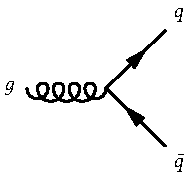
\includegraphics[width=0.7\textwidth]{gluon_quark_vertex}
%		\caption{\label{fig:gluon_quark_vertex}}
	\end{subfigure}%
	\begin{subfigure}[b]{0.33\linewidth}
		\centering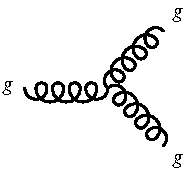
\includegraphics[width=0.7\textwidth]{gluon_vertex}
%		\caption{\label{fig:gluon_vertex}}
	\end{subfigure}	
	\begin{subfigure}[b]{0.33\linewidth}
		\centering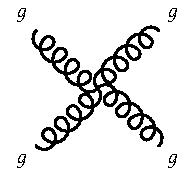
\includegraphics[width=0.7\textwidth]{gluon_quartic_vertex}
%		\caption{\label{fig:gluon_quartic_vertix}}
	\end{subfigure}
	\caption{Possible vertices in \gls{qcd}.}
	\label{fig:qcd_vertices}
\end{figure}

\subsubsection{Electroweak interaction}
\label{sec:ewk_interaction}

During the 1960s, Glashow, Weinberg and Salam~\cite{GLASHOW1961579,PhysRevLett.19.1264,Salam1959} developed a unified theory of the electromagnetic and weak interactions, based on the $SU(2)_\mathrm{L}\otimes U(1)_Y$ symmetry group. Known already experimentally from the Wu experiment~\cite{PhysRev.105.1413} in 1956, weak interaction violates parity, \ie the symmetry transformations have to act differently on the left-handed and right-handed fermion fields. The left- and right-handed components of a fermion field can be projected out using
\begin{equation}
	\psi_\mathrm{L} = \frac{1-\gamma^5}{2}\psi , \ \ \qquad 	\psi_\mathrm{R} = \frac{1+\gamma^5}{2}\psi,
\end{equation}
with $\gamma^5 = i\gamma^0\gamma^1\gamma^2\gamma^3$. As the weak interaction only acts on left-handed fermions, they can be ordered as $SU(2)$ doublets
\begin{equation}
	\begin{pmatrix}
		\nu_e \\
		e
	\end{pmatrix}_\mathrm{L},
	\quad
	\begin{pmatrix}
		u \\
		d
	\end{pmatrix}_\mathrm{L},
	\qquad
	\begin{pmatrix}
		\nu_\mu \\
		\mu
	\end{pmatrix}_\mathrm{L},
	\quad
	\begin{pmatrix}
		c \\
		s
	\end{pmatrix}_\mathrm{L},
	\qquad
	\begin{pmatrix}
		\nu_\tau \\
		\tau
	\end{pmatrix}_\mathrm{L},
	\quad
	\begin{pmatrix}
		t \\
		b
	\end{pmatrix}_\mathrm{L}.
\end{equation} 
The quantum number associated with $SU(2)$ symmetry transformations is called weak isospin $I$ with the third component $I_3$. Fermion doublets have $I=1/2$, with the upper component having $I_3 = 1/2$ and the lower component $I_3=-1/2$. Right-handed fermion fields have $I=0$, \ie are singlet states in weak isospin space
\begin{equation}
	e_\mathrm{R},u_\mathrm{R},d_\mathrm{R}, \qquad \mu_\mathrm{R},c_\mathrm{R},s_\mathrm{R}, \qquad \tau_\mathrm{R},t_\mathrm{R},b_\mathrm{R}, 
\end{equation}
and thus do not couple to the weak interaction. In the electroweak theory, neutrinos are assumed to be strictly massless, therefore no right-handed neutrino singlets exist. 

The fermion doublets can be written in a free Lagrangian similar to \cref{eq:free_lagrangian,eq:dirac_lagrangian},
\begin{equation}
	\Lagr = \bar{\psi}_\mathrm{L}i\gamma^\mu\partial_\mu\psi_\mathrm{L},
\end{equation}
with one crucial difference---the omission of the fermion masses. As $\bar{\psi}\psi = \bar{\psi}_\mathrm{L}\psi_\mathrm{R} + \bar{\psi}_\mathrm{R}\psi_\mathrm{L}$, mass terms would mix left- and right-handed terms and break gauge invariance. \Cref{sec:ssb} will illustrate how fermion masses will instead be generated in the electroweak theory. For left-handed fermion fields, local $SU(2)_\mathrm{L}$ transformations can be written as
\begin{equation}
	\psi_\mathrm{L} \rightarrow \mathrm{exp}\left(ig_2\alpha^a\frac{\sigma^a}{2}\right)\psi_\mathrm{L},
\end{equation}  
where $g_2$ is the coupling constant, $\alpha^a$ (with $a=1,2,3$) are real parameters and the Pauli matrices $\sigma^a$ are the generators of $SU(2)_\mathrm{L}$. By introducing the covariant derivative $\codiff_\mu = \partial_\mu + ig_2\frac{\sigma^a}{2}W^a_\mu$ and including the usual kinetic term for the gauge fields, the Lagrangian becomes invariant under $SU(2)_\mathrm{L}$ transformations and reads
\begin{equation}
	\Lagr = \bar{\psi}_\mathrm{L}i\gamma^\mu\codiff_\mu\psi_\mathrm{L} - \frac{1}{4}W^a_{\mu\nu}W^{\mu\nu,a},
\end{equation}
with the gauge field strength tensors $W^a_{\mu\nu} = \partial_\mu W^a_\nu - \partial_\nu W^a_\mu + g_2 \epsilon^{abc}W^b_\mu W^c_\nu$, where $\epsilon^{abc}$ are the structure constants. As previously in the case of \gls{qcd}, the non-Abelian structure of the symmetry group causes self-interactions of the gauge fields.

In order to include electromagnetic interactions, the weak isospin group is extended with the $U(1)_Y$, corresponding to the multiplication of a phase factor $e^{i\alpha\frac{Y}{2}}$ to each of the preceding doublets and singlets. Here, $Y$ is the weak hypercharge as given by the Gell-Mann--Nishijima relation~\cite{Gell-Mann1956,10.1143/PTP.13.285,10.1143/PTP.10.581},
\begin{equation}
	Q = I_3 + \frac{Y}{2},
	\label{eq:gell-mann-nishijima}
\end{equation}
with $Q$ the electric charge.
As will be discussed in \cref{sec:ssb}, the spontaneous breaking of the \mbox{$SU(2)_\mathrm{L}\otimes U(1)_Y$} gauge symmetry will recover the electromagnetic gauge group $U(1)_\mathrm{em}$~\cite{Peskin:1995ev}.

By modifying the covariant derivative to include a $U(1)_Y$ gauge field and ensuring that $U(1)_Y$ acts the same on left-handed and right-handed fermions, it becomes $\codiff_\mu = \partial_\mu + ig_2\frac{\sigma^a}{2}W^a_\mu + ig_1\frac{Y}{2}B_\mu$ for left-handed fermions and $\codiff_\mu = \partial_\mu + ig_1\frac{Y}{2}B_\mu$ for right-handed fermions. The full electroweak Lagrangian then is
\begin{equation}
\begin{split}
	\Lagr_\mathrm{electroweak} = & \sum_j{\bar{\psi}_\mathrm{L}^j i \gamma^\mu \left(\partial_\mu -ig_2\frac{\sigma^a}{2} W^a_\mu + ig_1 \frac{Y}{2} B_\mu \right) \psi^j_\mathrm{L}} \\
	& + \sum_j{\bar{\psi}_\mathrm{R}^j i \gamma^\mu \left(\partial_\mu + ig_1 \frac{Y}{2} B_\mu \right) \psi^j_\mathrm{R}}, 
\end{split}
\end{equation}
where $B_{\mu\nu} = \partial_\mu B_\nu - \partial_\nu B_\mu$, and the two sums run over the left- and right-handed fermions, respectively.

\subsubsection{Spontaneous symmetry breaking}
\label{sec:ssb}

In the electroweak theory a total of three vector fields $W^a_\mu$ and one vector field $B_\mu$ are associated with the gauge groups $SU(2)_\mathrm{L}$ and $U(1)_Y$, respectively. As has been shown explicitly through the example of \gls{qed} in \cref{sec:gauge_principle}, the gauge fields need to be massless for the resulting Lagrangian to be gauge invariant under the respective symmetry group. In addition, the electroweak symmetry group does not allow for fermion masses. Both gauge bosons of the weak interaction and the fermions are, however, manifestly massive, hence the electroweak symmetry has to be broken in the \gls{sm}.

The spontaneous symmetry breaking of the $SU(2)_\mathrm{L}\otimes U(1)_Y$ gauge group to $U(1)_\mathrm{em}$ is achieved through the Brout--Englert--Higgs   mechanism~\cite{PhysRevLett.13.321,PhysRevLett.13.508,PhysRev.145.1156}. In the SM, an isospin doublet of complex scalar fields, called Higgs doublet, is introduced
\begin{equation}
	\Phi(x) = \begin{pmatrix}
		\phi^+(x) \\
		\phi^0(x)
	\end{pmatrix}.
\end{equation}
The Higgs doublet has hypercharge $Y=1$, hence according to \cref{eq:gell-mann-nishijima}, $\phi^+$ has electric charge +1 while $\phi^0$ is electrically neutral. With the covariant derivative introduced in \cref{sec:ewk_interaction}, the Higgs doublet gets an associated part in the SM Lagrangian, 
\begin{equation}
	\Lagr_h = (\codiff_\mu\Phi)^\dagger(\codiff^\mu\Phi) - V(\Phi),
	\label{eq:higgs_lagrangian}
\end{equation}
where $V(\Phi)$ is a gauge invariant potential
\begin{equation}
	V(\Phi) = -\mu^2\Phi^\dagger\Phi + \frac{\lambda}{4}(\Phi^\dagger\Phi)^2.
	\label{eq:higgs_potential}
\end{equation}
For positive and real parameters $\mu^2$ and $\lambda$, this potential has the form of a \textit{Mexican hat} and an infinite number of minima for field configurations with $\Phi^\dagger\Phi=2\mu^2/\lambda$. In the vacuum, \ie in the ground state of the theory with minimal potential energy of the field, one of these minima is chosen such that the Higgs  receives a \gls{vev},
\begin{equation}
	\braket{\Phi} = \frac{1}{\sqrt{2}}\begin{pmatrix}
		0 \\
		v
	\end{pmatrix} \qquad \textrm{with} \quad v = \frac{2\mu}{\sqrt{\lambda}} \approx \SI{246}{\GeV}.
	\label{eq:higgs_vev}
\end{equation}
This is neither invariant under a $SU(2)_\mathrm{L}$ transformation of the form $U = \mathrm{exp}(i\alpha^a\frac{\sigma^a}{2})$, nor under a $U(1)_Y$ transformation of the form $\mathrm{exp}(i\alpha\frac{Y}{2})$. Thus, the Lagrangian has a symmetry that the vacuum state does not have. As the \gls{vev} of $\phi^+$ vanishes and $\phi^0$ is invariant under $U(1)_\mathrm{em}$, the symmetry group $SU(2)_\mathrm{L}\otimes U(1)_Y$ is therefore spontaneously broken down to $U(1)_\mathrm{em}$~\cite{Brock:1354959}.

The Higgs doublet can be expressed as excitations around the ground state
\begin{equation}
	\Phi(x) = \frac{1}{\sqrt{2}} \begin{pmatrix}
		\phi_1(x)+i\phi_2(x) \\
		v + h(x) + i\chi(x)
	\end{pmatrix},
	\label{eq:higgs_expansion}
\end{equation}
where $h$, $\chi$, $\phi_1$ and $\phi_2$ are real-valued scalar fields with vanishing \glspl{vev}. Inserting 
\cref{eq:higgs_expansion} back into the potential $V(\Phi)$ in \cref{eq:higgs_potential} yields
\begin{equation}
	V = \mu^2h^2 + \frac{\mu^2}{v} h (h^2 + \chi^2 + \phi_1^2+\phi_2^2)+ \frac{\mu^2}{4v^2}(h^2 + \chi^2 + \phi_1^2 + \phi_2^2),
	\label{eq:higgs_potential_excitation}
\end{equation}
where only \textit{h} gets a mass term, thus describing an electrically neutral scalar particle with mass $m_h = \sqrt{2}\mu$.
The remaining scalar fields remain massless, which is in accordance with the Nambu-Goldstone theorem~\cite{Nambu:1960tm,Goldstone:1961eq}, stating that every spontaneously broken continuous symmetry generates a massless Goldstone boson. These bosons are unphysical and can be gauged away through a $SU(2)_\mathrm{L}$ transformation, such that the expansion around the vacuum from \cref{eq:higgs_expansion}, involves only the physical scalar $h(x)$ in the so-called \textit{unitary gauge}.
\begin{figure}
	\centering
	\begin{subfigure}[b]{0.33\linewidth}
		\centering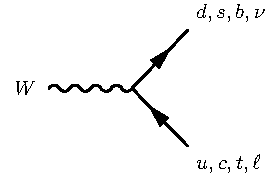
\includegraphics[width=0.8\textwidth]{w_fermion_vertex}
	\end{subfigure}%
	\begin{subfigure}[b]{0.33\linewidth}
		\centering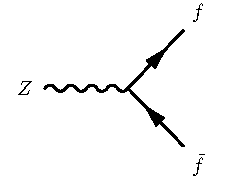
\includegraphics[width=0.8\textwidth]{z_fermion_vertex}
	\end{subfigure}	
	\begin{subfigure}[b]{0.33\linewidth}
		\centering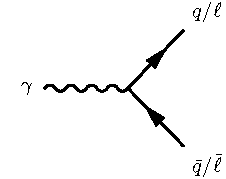
\includegraphics[width=0.8\textwidth]{gamma_fermion_vertex}
	\end{subfigure}
	\par\medskip
	\begin{subfigure}[b]{0.33\linewidth}
		\centering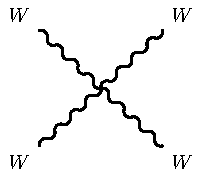
\includegraphics[width=0.7\textwidth]{w_boson_quartic_vertex}
	\end{subfigure}%
	\begin{subfigure}[b]{0.33\linewidth}
		\centering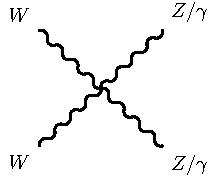
\includegraphics[width=0.7\textwidth]{wz_boson_quartic_vertex}
	\end{subfigure}	
	\begin{subfigure}[b]{0.33\linewidth}
		\centering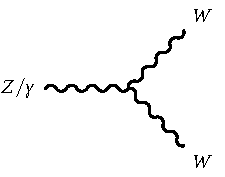
\includegraphics[width=0.8\textwidth]{w_boson_cubic_vertex}
	\end{subfigure}
	\caption{Possible vertices in the electroweak interaction.}
	\label{fig:ewk_vertices}
\end{figure}


Inserting \cref{eq:higgs_expansion} and the potential $V$ from \cref{eq:higgs_potential_excitation} back into the Lagrangian $\Lagr_h$ in \cref{eq:higgs_lagrangian} leads to mass terms for the gauge fields through their couplings to the \textit{h} field. The \textit{physical} fields corresponding to the physically observable $W^\pm$, $Z$ and $\gamma$ bosons in the electroweak theory are then given by the linear combinations
\begin{align*}
	W^\pm_\mu 	& = \frac{1}{\sqrt{2}}(W^1_\mu\mp i W^2_\mu) 				& \textrm{with} \quad m_W  & = \frac{g_2}{2}v, \\
	Z_\mu 		& = \cos\theta_W W_\mu^3 - \sin\theta_W B_\mu 	& \textrm{with} \quad m_Z  & = \frac{1}{2}\sqrt{g_1^2+g_2^2}v, \\
	A_\mu 		& = \sin\theta_W W_\mu^3 + \cos\theta_W B_\mu 	& \textrm{with} \quad m_A  & = 0,
\end{align*}
where $\theta_W$ is the weak mixing angle. It is related to the masses of the $W$ and $Z$ bosons, and the electroweak coupling constants by
\begin{equation}
	\cos{\theta_W} = \frac{g_2}{\sqrt{g_1^2 + g_2^2}} = \frac{m_W}{m_Z}.
\end{equation} 

%The Higgs potential can then be written as
%\begin{equation}
%	V = \mu^2h^2 + \frac{\mu^2}{v} h (h^2 + \chi^2 + \phi_1^2+\phi_2^2)+ \frac{\mu^2}{4v^2}(h^2 + \chi^2 + \phi_1^2 + \phi_2^2),
%\end{equation}
%where only $h$ gets a mass term, thus describing an electrically neutral scalar particle with mass $m_h = \sqrt{2}\mu$. The remaining scalar fields remain massless, in accordance with the Nambu-Goldstone theorem~\cite{Nambu:1960tm,Goldstone:1961eq}, stating that every spontaneously broken continuous symmetry generates a massless Goldstone boson. These bosons are unphysical and can be gauged away through a $SU(2)_\mathrm{L}$ transformation, such that the expansion around the vacuum from \cref{eq:higgs_expansion} involves only the physical scalar $H(x)$,
%\begin{equation}
%	\Phi(x) = \frac{1}{\sqrt{2}} \begin{pmatrix}
%		0 \\
%		v + h(x)
%	\end{pmatrix}.	
%\end{equation}
%The gauge transformation bringing \cref{eq:higgs_expansion} into the above form is called the \textit{unitary gauge}~\cite{Brock:1354959}. In this gauge, the Higgs potential from \cref{eq:higgs_potential} has the form
%\begin{equation}
%	V = \frac{m_h^2}{2} h^2 + \frac{m_h^2}{2v} h^3 + \frac{m_h^2}{8v^2} h^4,
%\end{equation}
%containing cubic and quartic self-interactions of the Higgs field proportional to $m^2_h$. Inserting the excitation around the vacuum state in the kinetic term of $\Lagr_\mathrm{h}$ yields mass terms for the vector bosons,
%\begin{equation}
%	\Lagr_{h} \propto \frac{v^2}{8}g^2_2\left(W_\mu^1W^{1,\mu} + W_\mu^2W^{2,\mu}\right) + \frac{v^2}{8} \begin{pmatrix}
%		W^3_\mu & B_\mu
%	\end{pmatrix}
%	\begin{pmatrix}
%		g_2^2 & g_1g_2   \\
%		g_1g_2 & g_1^2
%	\end{pmatrix}
%	\begin{pmatrix}
%		W^{3,\mu} \\
%		B^\mu
%	\end{pmatrix}.
%\end{equation}
%Instead of expressing the Lagrangian in terms of the fields $W^a_\mu$ and $B_\mu$ that make the original gauge invariance manifest, it can also be written in terms of the \textit{physical} fields that correspond to the physical $W^\pm$, $Z$ and $\gamma$ bosons in the electroweak theory,
%\begin{align*}
%	W^\pm_\mu 	& = \frac{1}{\sqrt{2}}(W^1_\mu\mp i W^2_\mu) 				& \textrm{with} \quad m_W  & = \frac{g_2}{2}v, \\
%	Z_\mu 		& = \frac{1}{\sqrt{g_1^2+g_2^2}}(g_2W^3_\mu - g_1 B_\mu) 	& \textrm{with} \quad m_Z  & = \frac{\sqrt{g_1^2+g_2^2}}{2}v, \\
%	A_\mu 		& = \frac{1}{\sqrt{g_1^2+g_2^2}}(g_1W^3_\mu + g_2 B_\mu) 	& \textrm{with} \quad m_A  & = 0.
%\end{align*}
%It is worth noting, that the massless photon field $A_\mu$ associated with the electromagnetic $U(1)_\mathrm{em}$ gauge symmetry is automatically recovered. All possible vertices between fermions and the physical electroweak gauge bosons are shown in \cref{fig:ewk_vertices}. The change of basis from $(W^3_\mu, B_\mu)$ to $(Z_\mu,A_\mu)$~\cite{Peskin:1995ev} can also be written as a basis rotation with the weak mixing angle $\theta_W$, \improvement{Write somewhere SU2xU1 to U1 breakdown}
%\begin{equation}
%	\begin{pmatrix}
%		Z_\mu \\
%		A_\mu
%	\end{pmatrix} =
%	\begin{pmatrix}
%		\cos{\theta_W} & \sin{\theta_W} \\
%		- \sin{\theta_W} & \cos{\theta_W}
%	\end{pmatrix}
%	\begin{pmatrix}
%		W^3_\mu \\
%		B_\mu
%	\end{pmatrix} \qquad \textrm{with } \cos{\theta_W} = \frac{g_2}{\sqrt{g_1^2 + g_2^2}} = \frac{m_W}{m_Z}.
%\end{equation}

\begin{figure}
	\centering
	\begin{subfigure}[b]{0.33\linewidth}
		\centering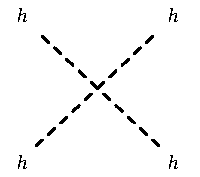
\includegraphics[width=0.75\textwidth]{h_boson_quartic_vertex}
	\end{subfigure}%
	\begin{subfigure}[b]{0.33\linewidth}
		\centering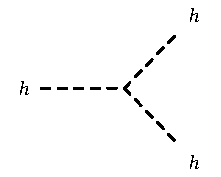
\includegraphics[width=0.85\textwidth]{h_boson_cubic_vertex}
	\end{subfigure}%
	\begin{subfigure}[b]{0.33\linewidth}
		\centering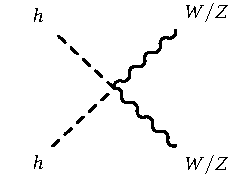
\includegraphics[width=0.9\textwidth]{h_boson_digauge_vertex}
	\end{subfigure}
	\par\medskip
	\begin{subfigure}[b]{0.33\linewidth}
		\centering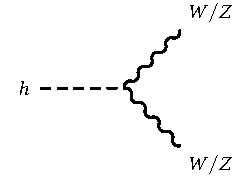
\includegraphics[width=0.9\textwidth]{h_boson_gauge_vertex}
	\end{subfigure}%
	\begin{subfigure}[b]{0.33\linewidth}
		\centering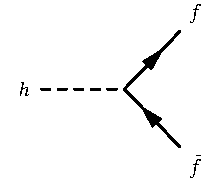
\includegraphics[width=0.85\textwidth]{h_boson_fermion_vertex}
	\end{subfigure}	
	\caption{Possible vertices involving the Higgs boson.}
	\label{fig:higgs_vertices}
\end{figure}

In the \gls{sm} the $W^\pm$ and $Z$ bosons thus acquire masses through spontaneous breaking of the electroweak gauge symmetry $SU(2)_\mathrm{L}\otimes U(1)_Y$ through the Higgs mechanism. The massless photon field $A_\mu$ associated with the electromagnetic $U(1)_\mathrm{em}$ gauge symmetry is automatically recovered. All possible vertices between fermions and the physical electroweak gauge bosons are shown in \cref{fig:ewk_vertices}. 

Furthermore, the masses of fermion fields are related to gauge-invariant Yukawa interactions with the Higgs field. For one fermion generation, the respective Yukawa terms in the Lagrangian are
\begin{equation}
	\Lagr_\mathrm{Yukawa,gen} = - \lambda_\ell \bar{L}_\mathrm{L}\Phi\ell_\mathrm{R} - \lambda_d \bar{Q}_\mathrm{L}\Phi d_\mathrm{R} - \lambda_u \bar{Q}_\mathrm{L} \Phi^\dagger u_\mathrm{R} + \mathrm{h.c.},
\end{equation}
where $\lambda_f$ with $f = \ell,d,u$ are the dimensionless Yukawa couplings and $L_\mathrm{L} = (\nu_\mathrm{L},\ell_\mathrm{L})^T$ and $Q_\mathrm{L} = (u_\mathrm{L},d_\mathrm{L})^T$ are the left-handed lepton and quark doublets, respectively. The non-vanishing \gls{vev} of the Higgs field then gives rise to fermion mass terms of the form 
\begin{equation}
 m_f = \lambda_f \frac{v}{\sqrt{2}},
\end{equation}
yielding fermion couplings to the Higgs field proportional to the fermion masses $m_f$. All \gls{sm} interaction vertices involving the Higgs boson are shown in \cref{fig:higgs_vertices}.
% The \gls{vev} of the Higgs field then gives rise to fermion mass terms in the Lagrangian, which, in the unitary gauge, yields for a single fermion generation
%\begin{equation}
% 	\Lagr_\mathrm{Yukawa, gen} = - \sum_{f=\ell,d,u}{\left(m_f\bar{\psi}_f\psi_f + \frac{m_f}{v}h\bar{\psi}_f\psi_f\right)} \qquad \textrm{with} \quad m_f = \frac{1}{\sqrt{2}}\lambda_f v.
%\end{equation}

When introducing all three fermion generations, additional Yukawa terms mixing fermions of different generations appear in the Lagrangian~\cite{Brock:1354959}. The terms involving quark fields can be parametrised using the \gls{ckm} matrix $V_\mathrm{CKM}$~\cite{PhysRevLett.10.531,CKM:1973fv}, quantifying the transition probability between quark generations. Since no right-handed neutrinos exist in the SM, no generation mixing in the lepton sector occurs and hence no neutrino mass terms are allowed in the \gls{sm}. Neutrino oscillations have, however, been observed experimentally, thus at least two massive neutrino generations need to exist. Their mixing can then be described with the \gls{pmns} matrix~\cite{PMNS:1962mu}, allowing neutrinos to acquire mass \eg through the see-saw mechanism~\cite{Brdar:2019iem}.
 
\subsection{Renormalisation and divergencies}
\label{ch:renormalisation}

At lowest order in the perturbative expansion, the momenta of the internal lines in the Feynman diagrams are fixed by the external particles. For higher orders where the diagrams involve loops, the momenta of the internal lines need to be integrated over as they are not fixed by energy-momentum conservation. Some examples of loop corrections to propagators and vertices are shown in \cref{fig:loop_corrections}. As each vertex in the Feynman diagrams is associated with a coupling constant that is usually much smaller than 1 (apart from the non-perturbative regime of \gls{qcd}), higher orders in the perturbative expansion contribute less and less to the total amplitude of the full expansion.

\begin{figure}
	\centering
	\begin{subfigure}[b]{0.33\linewidth}
		\centering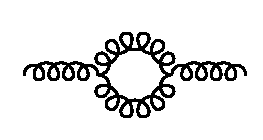
\includegraphics[width=0.85\textwidth]{gluon_loop}
		\caption{\label{fig:gluon_loop}}
	\end{subfigure}%
	\begin{subfigure}[b]{0.33\linewidth}
		\centering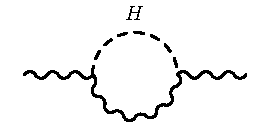
\includegraphics[width=0.85\textwidth]{wz_propagator}
		\caption{\label{fig:wz_propagator}}
	\end{subfigure}	
	\begin{subfigure}[b]{0.33\linewidth}
		\centering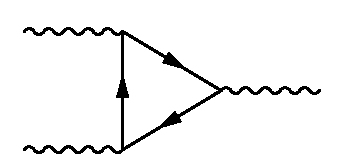
\includegraphics[width=0.85\textwidth]{cubic_vertex}
		\caption{\label{fig:cubic_vertex}}
	\end{subfigure}
	\caption{Examples of loop corrections to (a) the gluon propagator, (b) the $W$ or $Z$ propagator and (c) the cubic gauge boson vertex.}\label{fig:loop_corrections}
\end{figure}

The momentum integrals in loop corrections, however, lead to \textit{ultraviolet divergencies} for large momenta. In order to eliminate the divergencies, the integrals have to be \textit{regularised}, \eg by applying a cut-off scale $\Lambda$ or calculating the integrals in a number $D = 4-\epsilon$ of dimensions where they converge. The potential divergencies are then absorbed in parameters of the Lagrangian, such as coupling constants and masses, after which the regulator is removed (\eg $\epsilon\rightarrow 0$) again and a \textit{renormalisation} procedure is applied, replacing the bare parameter values with the physical, measured values~\cite{Brock:1354959}. Renormalisation effectively absorbs the effects of quantum fluctuations acting on much smaller scales than the scale of the given problem in the parameters of the theory.
\improvement{Mass dimension needs to be < 4}
As Veltmann and t'Hooft~\cite{THOOFT1972189,THOOFT1971173} have shown, all Yang-Mills theories with massive gauge fields are renormalisable, making the \gls{sm} as a whole a renormalisable theory.  

\section{Supersymmetry}

Originally developed in the late 1960s and early 1970s as an attempt to combine the Poincaré group with internal symmetries into a single symmetry group~\cite{kane2000the}, \glsfirst{susy} is a class of theories transforming fermionic states into bosonic ones, and vice-versa. Since its theoretical discovery, driven purely by theoretical developments rather than by pressure of existing data~\cite{kane2000the}, \gls{susy} was found to have far-reaching phenomenological consequences that could solve some of the shortcomings of the \gls{sm}. 

This section starts with an overview of these shortcomings and illustrates how they could be solved by supersymmetric theories. This is followed by an introduction to the mathematical description and phenomenological consequences of \gls{susy}. While the following sections are intended to highlight the most important concepts and relations, a much more complete and detailed introduction to \gls{susy} can be found in \references\cite{Martin:1997ns,Bustamante:2009us}.

%Among the properties a quantum field theory might possess to make it more mathematically tractable, one specific higher symmetry reveals particularly far-reaching implications; a symmetry relating fermions and bosons, known as \gls{susy}. In the following, the basic concepts of \gls{susy}, a class of theories that could solve some of the shortcomings of the \gls{sm}. 

%First, some of the shortcomings of the \gls{sm} are highlighted, and possible solutions through supersymmetric theories are illustrated.  highlighting some of the open questions of the SM. This is followed by an introduction to the mathematical description and phenomenological consequences of supersymmetric theories. The following sections are intended to highlight the most important concepts and relations, a much more complete and detailed introduction to \gls{susy} can be found in \references\cite{Martin:1997ns,Bustamante:2009us}.

\subsection{Shortcomings of the Standard Model}

Although the \gls{sm} is a remarkably successful theory able to predict and describe the interactions between elementary particles with unprecedented precision, there are still phenomena in nature that cannot be suitable understood within the theoretical framework of the \gls{sm}. 

Those limitations and open questions are the reason for numerous searches looking for new physics \gls{bsm}, such as the one presented in this thesis. Some of these open questions are described in the following. 

\subsubsection{Dark Matter}

The existence of \gls{dm}, \ie non-luminous and non-absorbing matter is nowadays well established~\cite{pdg2020}. Some of the earliest hints for the existence of \gls{dm} came from the observation that the rotation curves of luminous objects are not consistent with the expected velocities based on the gravitational attraction of the visible objects around them. Zwicky already postulated in 1933 the existence of \gls{dm}~\cite{Zwicky:437297} based on rotation curves of galaxies in the Coma cluster. In 1970, Rubin measured rotation curves of spiral galaxies~\cite{Rubin:1970zza}, revealing again a significant disagreement with the theoretically expected curves given the visible matter in the galaxies. Based on Newtonian dynamics, the circular velocity of stars outside the bulge of galaxies is expected to fall off with increasing radius as $v(r) \propto 1/\sqrt{r}$~\cite{Bertone:2004pz}. Rubin's observations, however, revealed that the velocities of stars outside the bulge stay approximately constant, strongly suggesting the existence of a non-luminous (or \textit{dark}) matter halo around the galaxies. Surveys of galaxy clusters and observations of gravitational lensing effects \eg in the bullet cluster~\cite{Clowe:2006eq} or the Abell 1689 cluster~\cite{Taylor:1998uk} have since then further consolidated the existence of large accumulations of non-luminous mass in the universe.

The anisotropies in \gls{cmb}, studied by the COBE~\cite{Bennett:1996ce,COBE}, WMAP~\cite{WMAP2,WMAP1} and Planck missions~\cite{Planck} are well described by the \gls{lcdm} model~\cite{Liddle:1976476}, which includes a density for cold dark matter. Planck's latest results~\cite{Aghanim:2018eyx} for the cold \gls{dm} relic density and baryonic density of
\begin{align}
\begin{split}
	\Omega_c h^2 &= 0.1200\pm0.0012, \\
	\Omega_b h^2 &= 0.02237\pm0.00015,
\end{split}
\end{align}
respectively, suggest that ordinary baryonic matter only makes up $\sim 4.9\%$ of the universe's matter content, while \gls{dm} accounts for $\sim 26.1\%$\footnote{The remaining $\sim 69\%$ are taken up by \textit{dark energy}, the nature of which is still an open question.}.

Candidates for cold \gls{dm} need to satisfy certain conditions: they have to be stable on cosmological timescales (otherwise they would have decayed by now), they have to couple only very weakly to the electromagnet interaction (if at all, otherwise they would be luminous matter) and they need to have the right relic density. Analyses of structure formations in the Universe have furthermore shown that most \gls{dm} should have been \textit{cold}, \ie non-relativistic at the beginning of galaxy formation~\cite{Bertone:2004pz}. Candidates for \gls{dm} particles are \eg sterile neutrinos, axions, primordial black holes, or \glspl{wimp}.

In the SM, the only \gls{dm} candidate particle is the neutrino. Given the upper limits on the neutrino masses, an upper bound on their relic density can be computed, revealing that neutrinos are not abundant enough to be a dominant component of \gls{dm}~\cite{Bertone:2004pz}. Furthermore, due to their low masses, neutrinos would still have been relativistic particles at the beginning of galaxy formation, preventing the \textit{bottom-up}\footnote{The \textit{bottom-up} structure formation begins with small objects that subsequently merge into ever larger structures and is the structure formation process favoured in a universe dominated by cold \gls{dm}.} structure formation favoured by a cold \gls{dm} dominated universe.

 Many \gls{bsm} theories naturally predict new \glspl{wimp} with masses in the GeV to TeV range. In many SUSY models with exact R-parity conservation (a quantity introduced in \cref{sec:rparity}), the lightest supersymmetric particle is neutral and stable and could be a good candidate for \gls{dm}.

\subsubsection{Unification of forces}


Although the \gls{sm} provides a good description of nature up to the energy scale probed with today's accelerators, some of its peculiar aspects hint to a more fundamental theory. A prominent example is the question why the electric charges of the electrons and the charges of the quarks of the protons and neutrons in the nuclei exactly cancel, making for electrically neutral atoms~\cite{Brock:1354959}. Or in other words: why are the charges of all observed particles simple multiples of the fundamental charge? And why are they quantised in the first place?

An explanation to many of these peculiarities comes naturally when describing the \gls{sm} as a unified theory with a single non-Abelian gauge group, \eg $SU(5)$~\cite{PhysRevLett.32.438}. The larger symmetry group with a single coupling constant is then thought to be spontaneously broken at very high energy, such that the known \gls{sm} interactions are recovered at the lower energies probed in today's experiments. In such a \gls{gut}, the particles in the \gls{sm} are arranged in anomaly-free\footnote{In the sense that loop corrections do not break symmetries the Lagrangian has.} irreducible representations of the gauge group, thereby \eg naturally ensuring the fractional charges of quarks~\cite{Peskin:1995ev}.
\begin{figure}
\floatbox[{\capbeside\thisfloatsetup{capbesideposition={right,center},capbesidewidth=0.4\textwidth}}]{figure}[\FBwidth]
{\caption{Evolution of the inverse coupling constants in the \gls{sm} (dashed lines) and the \gls{mssm} (solid lines) in function of the energy scale $Q$. In the \gls{mssm}, the masses of the supersymmetric particles are treated as common threshold varied between $\SI{750}{\GeV}$ and $\SI{2.5}{\TeV}$. Figure taken from \reference\cite{Martin:1997ns}.}\label{fig:unification_forces}}
{\includegraphics[width=0.5\textwidth]{unification}}
\end{figure}

In the \gls{sm}, the coupling constants run towards each other with increasing energy scale, but never exactly meet. In the \glsfirst{mssm}, introduced in \cref{sec:mssm_intro}, the running couplings meet within their current uncertainties if the supersymmetric particles are at the $\SI{}{\TeV}$ scale, hinting that a supersymmetric \gls{gut} could be a good candidate for describing physics at the unification scale. \Cref{fig:unification_forces} shows that the running coupling constants in the \gls{mssm} are modified such that they meet at $\SI{e16}{\GeV}$.

\subsubsection{The Hierarchy Problem}

As the \gls{sm} is a renormalisable gauge theory, finite results are obtained for all higher-order loop corrections, making the \gls{sm} a theory that is in principle well-defined up to infinite energies. In renormalisation terms, this means that the cut-off scale $\Lambda$ is theoretically allowed to go to arbitrarily high values. It is clear though, that the \gls{sm} cannot be a complete theory of nature and that at some unknown high-energy scale $\Lambda$, \textit{new physics} has to appear. At the very least, a new theoretical framework becomes necessary at the Planck scale $M_P \approx \SI{e19}{\GeV}$~\cite{Bustamante:2009us}, where quantum gravitational effects can no longer be ignored.

The mass parameters of fermions and massive vector bosons are protected from large quantum corrections by chiral symmetry and gauge symmetry, respectively~\cite{Aitchison:2007fn}. The mass parameter of the scalar Higgs field, on the other hand, receives loop corrections proportional at least to the scale at which new physics sets in. The Yukawa coupling of the Higgs field to a fermion $f$ with mass $m_f$, depicted in \cref{fig:fermion_loop}, yields a one-loop correction term to the Higgs square mass~\cite{Bustamante:2009us} given by
\begin{align}
	\Delta m_h^2 = -\frac{\lambda_f^2}{8\pi^2} \Lambda^2 + \dots\, .
	\label{eq:fermion_correction}
\end{align}
The Higgs mass thus quadratically diverges with the scale $\Lambda$. If the \gls{sm} is to be valid up to the Planck scale, then $\Lambda = M_P$, and the correction to the Higgs squared mass becomes more than $10^{30}$ times larger than the expected value in the order of $(\SI{e2}{\GeV})^2$~\cite{Martin:1997ns}.
Similar quantum corrections arise from the Higgs quartic coupling to a heavy scalar boson $S$ with mass $m_S$, shown in \cref{fig:scal_loop}, yielding a one-loop correction~\cite{Bustamante:2009us} given by 
\begin{align}
	\Delta m_h^2 = \frac{\lambda_S}{16\pi^2}\Lambda^2 + \dots\, .
	\label{eq:scalar_correction}
\end{align}
In order to obtain the experimentally measured value of the Higgs mass, the quantum corrections to the bare Higgs parameter have to be tuned in such a way that they almost cancel, leading to a \textit{fine-tuning} problem that is considered to be unnatural.

Interestingly, the terms quadratically divergent in $\Lambda$ in \cref{eq:fermion_correction} and \cref{eq:scalar_correction} enter with opposite signs. If, for every fermionic loop, there are two bosonic loops with $\lambda_S = \lambda_f^2$, the quadratically diverging terms neatly cancel. As will be discussed, this is exactly the case in supersymmetric theories. Additional correction terms omitted above are at most logarithmic in $\Lambda$, and cancel if the scalar bosons and the fermion have the same masses (this is further discussed in \cref{sec:susy_breaking}).

\begin{figure}
	\centering
	\begin{subfigure}[b]{0.5\linewidth}
		\centering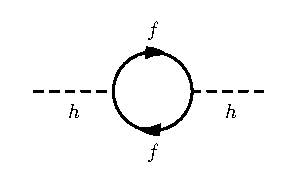
\includegraphics[width=0.75\textwidth]{fermion_loop}
		\caption{\label{fig:fermion_loop}}
	\end{subfigure}%
	\begin{subfigure}[b]{0.5\linewidth}
		\centering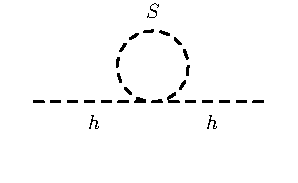
\includegraphics[width=0.75\textwidth]{scalar_loop}
		\caption{\label{fig:scal_loop}}
	\end{subfigure}	
	\caption{A massive fermion \subref{fig:fermion_loop} and a hypothetical massive scalar particle \subref{fig:scal_loop} coupling to the Higgs boson.}\label{fig:loop_corrections_higgs}
\end{figure}

%In SUSY, the Higgs mass is automatically protected from the large quantum corrections by the introduction of two complex scalar partners to each \gls{sm} fermion. The quantum corrections from a hypothetical heavy complex scalar particle $S$ with mass $m_S$ as in \cref{fig:scal_loop} yields a one-loop correction~\cite{Martin:1997ns} given by 
%\begin{align}
%	\Delta m_h^2 = \frac{\lambda_S}{16\pi^2}\left[\Lambda^2 - 2m_S^2\ln\left(\Lambda/m_S\right)+ \dots\right].
%	\label{eq:scalar_correction}
%\end{align}

%Interestingly, the corrections in \cref{eq:fermion_correction} and \cref{eq:scalar_correction} enter with opposite signs. Thus, if $\lambda_S = \vert\lambda_f\vert^2$, then the large quantum corrections neatly cancel and no excessive fine-tuning is needed. The requirement $\lambda_S = \vert\lambda_f\vert^2$ means that the fermions and their supersymmetric bosonic partners would have same masses. Such particles would have been discovered long ago in particle physics experiments, meaning that SUSY must be a broken symmetry (see \cref{sec:susy_breaking} for a discussion on \gls{susy} breaking) such that the supersymmetric particles acquire masses well above those of their \gls{sm} partners. 

\subsubsection{Anomalous magnetic moment of the muon}

One of the longest standing disagreements between experiment and theory in the \gls{sm} is the anomalous magnetic moment of the muon~\cite{pdg2020}. The magnetic moment of the muon $\vec{\mu}_\mu$ is related to its intrinsic spin $\vec{S}$ through the gyromagnetic ratio $g_\mu$ by
\begin{equation}
	\vec{\mu}_\mu = g_\mu \frac{q}{2m} \vec{S}.
\end{equation}
For a structureless spin-1/2 particle with mass $m$ and charge $q=\pm e$, the gyromagnetic ratio is $g_\mu = 2$~\cite{Bennett:2006fi}. Loop corrections coupling the muon spin to virtual fields cause small deviations, parameterised by the anomalous magnetic moment
\begin{equation}
	a_\mu = \frac{1}{2}(g_\mu-2).
\end{equation}
The anomalous magnetic moment can be precisely measured as well as predicted within the SM. A comparison between experimental data and theoretical prediction thus directly tests the \gls{sm} at quantum loop level and may hint to effects from new physics in case of discrepancies~\cite{baer_tata_2006}.
In the SM, the most dominant contribution to $a_\mu$ comes from \gls{qed} corrections involving photon and fermion loops.
An exemplary diagram is shown in \cref{fig:qed_anomalous_moment}. Weak contributions involving the heavy $W^\pm$, $Z$ and Higgs particles are suppressed by their masses~\cite{Aoyama:2020ynm}.
Although the contributions from \gls{qcd} are relatively small, they give rise to the main theoretical uncertainties as they cannot be calculated from first principles but rely either on data-driven calculations, or lattice \gls{qcd} evaluations~\cite{Aoyama:2020ynm}.

The muon \textit{g}--2 experiment at the Fermi National Accelerator Laboratory (FNAL)~\cite{Abi:2021gix} has recently measured the anomalous magnetic moment of the muon, updating the results from the E821 experiment at Brookhaven National Laboratory (BNL)~\cite{Bennett:2006fi} obtained in 2004. The combined experimental average of both experiments finds a deviation from the \gls{sm} expectation\footnote{The \gls{sm} value of $a_\mu$ adopted in \reference\cite{Abi:2021gix} relies on the data-driven evaluation of the hadronic contributions using $e^+e^-$ collider data, recommended by the muon \textit{g}--2 theory initiative~\cite{Aoyama:2020ynm}.} of
\begin{equation}
	\Delta a_\mu = a^\mathrm{exp}_\mu - a^\mathrm{SM}_\mu = (251\pm59)\times 10^{-11},
%	\Delta a_\mu = a^\mathrm{exp}_\mu - a^\mathrm{SM}_\mu = 261(63)(48)\times 10^{-11},
\end{equation}
which is quantified to have a significance of $4.2\sigma$~\cite{Abi:2021gix}. These results strongly hint at the existence of new physics beyond the \gls{sm}.

\begin{figure}
	\centering
	\begin{subfigure}[b]{0.33\linewidth}
		\centering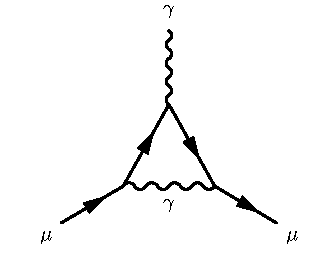
\includegraphics[width=1.0\textwidth]{qed_anomalous_moment}
		\caption{\label{fig:qed_anomalous_moment}}
	\end{subfigure}%
	\begin{subfigure}[b]{0.33\linewidth}
		\centering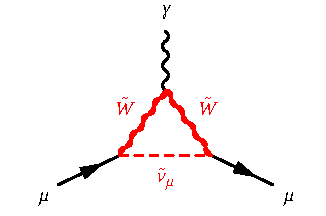
\includegraphics[width=1.0\textwidth]{susy_anomalous_moment_1}
		\caption{\label{fig:susy_anomalous_moment_1}}
	\end{subfigure}%
	\begin{subfigure}[b]{0.33\linewidth}
		\centering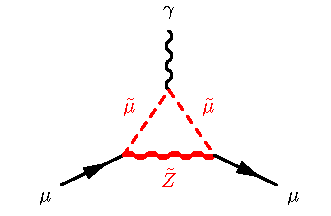
\includegraphics[width=1.0\textwidth]{susy_anomalous_moment_2}
		\caption{\label{fig:susy_anomalous_moment_2}}
	\end{subfigure}	
	\caption{Electromagnetic \subref{fig:qed_anomalous_moment} and supersymmetric \subref{fig:susy_anomalous_moment_1}, \subref{fig:susy_anomalous_moment_2} contributions to $a_\mu$. Supersymmetric particles are drawn in red. Adapted from~\reference\cite{baer_tata_2006}.}\label{fig:loop_corrections_anomalous_moment}
\end{figure}

In SUSY, additional Feynman diagrams exist, involving the supersymmetric partners of the muon, the muon neutrino and the electroweak gauge bosons, and thus the measured deviation in $a_\mu$ can easily be accommodated in many supersymmetric models~\cite{Czarnecki:2001pv,Feng:2001tr}. Two exemplary lowest-order diagrams involving supersymmetric particles (introduced in \cref{sec:mssm_particle_content}) are shown in \cref{fig:susy_anomalous_moment_1,fig:susy_anomalous_moment_2}.


\subsection{Supersymmetric Algebra}\label{sec:susy_algebra}

The Coleman--Mandula no-go theorem~\cite{PhysRev.159.1251} dictates that the symmetry group generating a consistent spacetime \gls{qft} must be the direct product of the internal symmetry group with the Poincaré group, which in principle rules out the possibility for SUSY. The Coleman--Mandula proof, however, assumes the new symmetry to be generated by bosonic integer spin generators. The Haag--Lopuszanski--Sohnius extension~\cite{Haag:1974qh} showed that the only possible way of non-trivially combining internal and spacetime symmetry groups is to use a Lie superalgebra and fermionic spin-1/2 generators.

A generator of supersymmetric transformations is thus an anti-commuting spinor $Q$ that turns fermionic states $\ket{f}$ into bosonic states $\ket{b}$ and vice-versa.
\begin{equation}
	Q\ket{f} = \ket{b}, \qquad \qquad \qquad Q\ket{b}=\ket{f}.
\end{equation}
As spinors are complex objects, $Q^\dagger$ is also a symmetry operator. Both $Q$ and $Q^\dagger$ are necessarily fermionic and thus must carry half-integer spin, in the simplest case spin-1/2, meaning that SUSY must be a spacetime symmetry, \ie a Poincaré symmetry. 
Thus, in order to obey the Haag--Lopuszanski--Sohnius loophole of the Coleman--Mandula theorem, and simultaneously allow for parity-violating interactions, the SUSY generators have to satisfy the following algebra of commutation and anti-commutation relations~\cite{Bustamante:2009us},
\begin{equation}
\begin{split}
	\{ Q,Q^\dagger \} & \quad = \quad  2\sigma_\mu P^\mu,\\
	\{ Q,Q \} &  \quad = \quad \{ Q^\dagger,Q^\dagger \} = 0, \\
	\left[P^\mu,Q \right] &  \quad = \quad \left[ P^\mu,Q^\dagger \right] = 0, \\
	\{ M^{\mu\nu}, Q \} & \quad = \quad \sigma^{\mu\nu} Q,\\
	\{ M^{\mu\nu},Q^\dagger \} & \quad = \quad \bar{\sigma}^{\mu\nu} Q^\dagger,
  \label{eq:commute}
\end{split}
\end{equation}
where $P^\mu$ is the four-momentum generator of spacetime translations, $\sigma_\mu = (\mathbb{1}_2,\sigma_i)$, $\bar{\sigma}_\mu = (\mathbb{1}_2,-\sigma_i)$ with $i=1,2,3$ and the Pauli matrices $\sigma_i$, and $\sigma^{\mu\nu} = \frac{i}{4}(\sigma^\mu\bar{\sigma}^\nu - \sigma^\nu\bar{\sigma}^\mu)$ as well as $\bar{\sigma}^{\mu\nu} = \frac{i}{4}(\bar{\sigma}^\mu\sigma^\nu - \bar{\sigma}^\nu\sigma^\mu)$. This is the simplest version of SUSY, called $N=1$ symmetry, as it introduces only one pair of generators. Supersymmetric theories with $N\geq 2$ pairs of generators also exist and generally have some theoretical advantages as \eg fewer divergencies in the case of $N=2$ or even no divergencies at all in the case of $N=4$~\cite{Bustamante:2009us}. SUSY models with $N\geq 2$, however, do not allow for parity violation and thus fail to describe the physics of the SM, disqualifying them from a phenomenological point of view~\cite{Bustamante:2009us}.

As both SUSY generators commute with spacetime translations (see \cref{eq:commute}), they also both commute with the squared mass operator $-P^2$. Consequently, particles related by the generators, called \textit{superpartners}, must have equal eigenvalues under $-P^2$, \ie they must have equal masses. Furthermore, the SUSY generators also commute with the gauge transformation generators, hence superpartners must have same electric charge, weak isospin and degrees of freedom in colour space~\cite{Martin:1997ns}.\improvement{Mention link to gravity}


\subsection{Supermultiplets}\label{sec:supermultiplets}

The \gls{sm} and \gls{susy} particles are arranged in irreducible representations of the SUSY algebra, called \textit{supermultiplets}, each containing both fermionic and bosonic states that are superpartners of each other. It can be shown that each supermultiplet has an equal number of fermion and boson degrees of freedom, $n_f = n_b$~\cite{Martin:1997ns}.

The simplest supermultiplet $\Psi$ that can be constructed contains a single Weyl fermion $\psi$ and two real scalars, described by a single complex field $\phi$, called the \textit{sfermion}. The Weyl fermion has two spin helicity states, hence $n_f=2$, and the complex scalar field has two components with $n_b=1$ each. An additional complex scalar field $F$, called \textit{auxiliary field} and not corresponding to a physical particle, has to be introduced in order to allow the SUSY algebra to close off-shell (where the energy-momentum relation does not hold)~\cite{Martin:1997ns}. The supermultiplet $\Psi$ thus reads
\begin{equation}
	\Psi = (\phi,\psi,F).
\end{equation}
Being a pure bookkeeping device, the auxiliary field does not propagate and can be eliminated on-shell with the equations of motion $F=F^*=0$. This supermultiplet is called a \textit{chiral} or \textit{scalar} supermultiplet~\cite{Martin:1997ns}. 

The next-simplest supermultiplet for which $n_f = n_b$ holds, is the \textit{vector} or \textit{gauge} supermultiplet~$\Phi$ containing a spin-1 gauge boson $A^\mu_a$, where $a$ is the index of the gauge group. In order for the theory to be renormalisable, this gauge boson must be massless before spontaneous breaking of the symmetry. As a massless spin-1 boson has two helicity states, $n_b = 2$, the superpartner, called \textit{gaugino}, must be a massless spin-1/2 Weyl fermion $\lambda_a$ with two helicity states such that $n_f = 2$~\cite{Martin:1997ns}. An auxiliary real bosonic field $D_a$ is needed in order to balance the degrees of freedom off-shell~\cite{Bustamante:2009us}, completing the supermultiplet to be
\begin{equation}
	\Phi = (\lambda_a,A^\mu_a,D_a).
\end{equation}
 Like the chiral auxiliary field, the gauge auxiliary field does not correspond to a physical particle and can be eliminated on-shell through its equations of motion~\cite{Martin:1997ns}.

\subsection{Supersymmetric Lagrangian}\label{sec:susy_lagrangian}

The simplest supersymmetric model that can be shown to realise the superalgebra is the massless, non-interacting Wess--Zumino model~\cite{Wess:1974tw} with the action~\cite{Bustamante:2009us,Martin:1997ns} 
\begin{equation}
\begin{split}
S & = \int \diff^4x(\Lagr_\mathrm{scalar} + \Lagr_\mathrm{fermion}), \\
	\Lagr_\mathrm{scalar} & = - \partial^\mu\phi^*\partial_\mu\phi, \\
	\Lagr_\mathrm{fermion} & = - i\psi^\dagger\bar{\sigma}^\mu\partial_\mu\psi , \\
	\label{eq:wess_zumino_free}
\end{split}
\end{equation}
with a massless complex scalar $\phi$ and a spin-1/2 fermion $\psi$, corresponding to a single chiral supermultiplet. As discussed in \cref{sec:supermultiplets}, in order for this Lagrangian to satisfy the supersymmetry off-shell where the equations of motion cannot be used, an auxiliary complex scalar field $F$ has to be added. The free Lagrangian~\cite{Bustamante:2009us} in the action thus reads
\begin{equation}
\begin{split}
	\Lagr_\mathrm{free} & = \Lagr_\mathrm{scalar} + \Lagr_\mathrm{fermion} + \Lagr_\mathrm{aux},  \qquad \mathrm{with} \quad \Lagr_\mathrm{aux} = F^{*i}F_i.
%	 & = \partial^\mu\phi^{*i}\partial_\mu\phi_i + i\psi^{\dagger i}\bar{\sigma}^\mu\partial_\mu\psi_i + F^{*i}F_i,
\end{split}
\label{eq:free_wess_zumino}
\end{equation} 
The auxiliary term $\Lagr_\mathrm{aux}$ implies the trivial equations of motion $F = F^* = 0$ which are needed to remove the auxiliary field in the on-shell case. The next step involves adding terms for non-gauge interactions for the chiral supermultiplets. Non-gauge interactions for chiral supermultiplets at most quadratic in the fermion fields can be achieved by introducing the term~\cite{Bustamante:2009us},
\begin{equation}
	\Lagr_\mathrm{int} = - \frac{1}{2}W^{ij}(\phi,\phi^*)\psi_i \psi_j + V(\phi,\phi^*) + c.c.,
	\label{eq:wess_zumino_int}
\end{equation}
where $W^{ij}$ is a holomorphic\footnote{A holomorphic function is a complex-valued function in one or more complex variables that is complex differentiable in a neighbourhood for every point of its domain.} function of the complex scalar fields $\phi_i$ of the form~\cite{Bustamante:2009us}
\begin{equation}
	W^{ij} = \frac{\partial^2 W}{\partial\phi_i\partial\phi_j}. 
\end{equation}
Here, $W$ is called the \textit{superpotential}. For the final Lagrangian to be renormalisable, the superpotential can at most be cubic~\cite{Bustamante:2009us}, and thus can be written as
\begin{equation}
	W = \frac{1}{2}m^{ij}\phi_i \phi_j + \frac{1}{6}y^{ijk}\phi_i \phi_j \phi_k,
	\label{eq:wess_zumino_potential}
\end{equation}
where $y^{ij}$ are the Yukawa couplings between the scalar and the two fermions, thus containing all non-gauge interactions. The term quadratic in the fields contains the fermion mass matrix $m^{ij}$, which is equal to the mass matrix of the scalar bosons due to supersymmetry, as will be shown below. Requiring $\Lagr_\mathrm{int}$ to be invariant under supersymmetry transformations further defines the potential $V$. The equations of motion of the auxiliary fields $F$ can be written as
\begin{equation}
	F_i = -\frac{\partial W(\phi)}{\partial \phi^i} = - W^*_i, \qquad F^{*i} = - \frac{\partial W(\phi)}{\partial \phi_i} = - W^i,
	\label{eq:wess_zumino_F}
\end{equation} 
which thus yields for the potential $V = W^*_iW^i = F_iF^{*i}$, allowing to write the Lagrangian without explicitly introducing the auxiliary fields. The full Lagrangian of the Wess-Zumino model with general chiral interactions between the scalar and fermion fields in the chiral supermultiplets~\cite{Bustamante:2009us} is then given by
\begin{equation}
	\Lagr = -\partial^\mu\phi^{*i}\partial_\mu\phi_i - i\psi^{\dagger i}\bar{\sigma}^\mu\partial_\mu\psi_i - \frac{1}{2} m^{ij}\psi_i \psi_j - \frac{1}{2} m_{ij}^* \psi^{\dagger i} \psi^{\dagger j} - \frac{1}{2} y^{ijk} \phi_i \psi_j \psi_k - \frac{1}{2} y^*_{ijk} \phi^{*i} \psi^{\dagger j} \psi^{\dagger k} - V(\phi,\phi^*),
	\label{eq:wess_zumino_lagrangian}
\end{equation}
obtained by adding the interaction term $\Lagr_\mathrm{int}$ from~\cref{eq:wess_zumino_int} to the free Lagrangian in~\cref{eq:wess_zumino_free} and inserting the expression for the superpotential from~\cref{eq:wess_zumino_potential} and the auxiliary fields from~\cref{eq:wess_zumino_F}.

The Lagrangian in \cref{eq:wess_zumino_lagrangian} immediately reveals that, as expected by supersymmetry, the masses of the fermions and bosons in the same supermultiplet are identical. In order to incorporate gauge supermultiplets and consider the interactions between fermions and gauge bosons observed in the SM, the usual minimal coupling rule has to be applied, replacing $\partial_\mu$ with $\codiff_\mu$. This leads to equation of motions for the auxiliary fields $D^a$
\begin{equation}
	D^a = -g(\phi^*T^a\phi),
\end{equation}
where $T^a$ are the generators of the gauge group and $g$ is the coupling constant~\cite{Bustamante:2009us}. The potential then becomes
\begin{equation}
	V(\phi,\phi^*) = F^{*i}F_i + \frac{1}{2} \sum_a{D^aD^a} = W^*_iW^i + \frac{1}{2}\sum_a{g^2_a(\phi^*T^a\phi)^2} ,
\end{equation}
where $a$ runs over the gauge groups that generally have differing gauge couplings~\cite{Bustamante:2009us}.


 
\subsection{The Minimal Supersymmetric Standard Model}\label{sec:mssm_intro}

The \gls{mssm} is the simplest $N=1$ supersymmetric extension of the \gls{sm} in the sense that it introduces a minimal set of additional particles.

\subsubsection{Particle content and interactions}\label{sec:mssm_particle_content}

The \gls{mssm} arranges all \gls{sm} particles in chiral (all the fermions and quarks) and gauge (all spin-1 bosons) supermultiplets. As supersymmetric partners (\textit{spartners}) have the same quantum numbers apart from spin, none of the \gls{sm} particles can be spartners of each other.
Thus, all spartners have to be new, unseen particles. \Cref{tab:particles_MSSM} summaries the names, notations and spins of all spartners introduced in the \gls{mssm}.
The naming convention is to prepend the names of the spartners of fermions with an 's' (\eg \textit{selectron}, \textit{stop}, ...) and append '-ino' to the names of the spartners of the bosons (\eg \textit{Wino}, \textit{Photino}, ...).
Supersymmetric particles (\textit{sparticles}) are generally denoted by adding a tilde to the symbol of \gls{sm} particles (\eg $\tilde{e}$, $\tilde{u}$, $\tilde{g}$). 

\begin{table}
	\centering
	\small
	\setlength\heavyrulewidth{0.2ex}
	\caption{Particle content of the \gls{mssm}. The spin refers to the spin of the spartner. Adapted from~\cite{Bustamante:2009us}.}
	\begin{tabular} {l l c}
		
		\toprule
		Particle & Spartner 0 & Spin \\ 
		\midrule 
		quarks $q$ & squarks $\tilde{q}$ & 0 \\
		$\rightarrow$ top $t$ & stop $\tilde{t}$ & \\
		$\rightarrow$ bottom $t$ & sbottom $\tilde{b}$ & \\
		$\dots$ & & \\
		leptons $\ell$ & sleptons $\tilde{\ell}$ & 0 \\
		$\rightarrow$ electron $e$ & selectron $\tilde{e}$ & \\
		$\rightarrow$ muon $\mu$ & smuon $\tilde{\mu}$ & \\
		$\rightarrow$ tau $\tau$ & stau $\tilde{\tau}$ & \\
		$\rightarrow$ neutrinos $\nu_\ell$ & stop $\tilde{\nu}_\ell$ & \\
		\midrule
		gauge bosons & gauginos & 1/2 \\
		$\rightarrow$ photon $\gamma$ & photino $\tilde{\gamma}$ & \\
		$\rightarrow$ boson $Z$ & Zino $\tilde{Z}$ & \\
		$\rightarrow$ boson $B$ & Bino $\tilde{B}$ & \\
		$\rightarrow$ boson $W$ & Wino $\tilde{W}$ & \\
		$\rightarrow$ gluon $g$ & gluino $\tilde{g}$ & \\
		\midrule
		Higgs bosons $H^{\pm,0}_i$ & higgsinos $\tilde{H}^{\pm,0}_i$ & 1/2 \\
		\bottomrule
	\end{tabular}\vspace{3mm}
	\label{tab:particles_MSSM}   
\end{table}

An important detail to note is that right-handed and left-handed fermions get their own chiral supermultiplets and thus have distinct spartners, as otherwise the preference of the weak interaction for left-handed particles would be violated. 
For example, left-handed and right-handed quarks ($q_\mathrm{L}$, $q_\mathrm{R}$) get two different spartners ($\tilde{q}_\mathrm{L}$, $\tilde{q}_\mathrm{R}$), denoted with an index L and R.
The index here refers to the handiness of the SM particle as scalar particles have only one helicity state. Additionally, the spartners of the left-handed and right-handed will mix to form physical mass eigenstates.

It is also worth asking why the spartners of SM particles are of lower spin in the first place, as \eg spin-1 spartners of the SM fermions could also have been considered. The introduction of spin-1 bosons would entail the introduction of new gauge interactions, rendering the \gls{mssm} non-minimal~\cite{Bustamante:2009us}. Furthermore, introducing spartners with spin greater than 1 would make the resulting theory non-renormalisable~\cite{Bustamante:2009us}.

In the \gls{mssm}, two Higgs doublets are needed in order to give masses to the up-type and down-type quarks via Yukawa couplings. A single Higgs field $h$ cannot be used for this as it would require Yukawa terms including the complex conjugate $h^*$, which is forbidden as the superpotential, being a holomorphic function of the fields, cannot depend on the complex conjugates of the same fields~\cite{Bustamante:2009us}. Additionally, the use of a single Higgs doublet would lead to gauge anomalies in the electroweak gauge symmetry~\cite{PhysRevD.6.429}. Instead two complex Higgs doublets with hypercharge $Y = \pm 1/2$ are used in the \gls{mssm}. The two Higgs doublets can be written as
\begin{equation}
	H_u = \begin{pmatrix}
		H^0_u \\
		H^-_u
	\end{pmatrix}, \qquad \qquad
	H_d = \begin{pmatrix}
		H^+_d \\
		H^0_d
	\end{pmatrix},
	\label{eq:Higgs_doublets}
\end{equation}

As illustrated in \cref{sec:susy_lagrangian} using the Wess--Zumino model, interactions are introduced using the superpotential. In the \gls{mssm}, the superpotential reads
\begin{equation}
	W_\mathrm{MSSM} = \bar{u}\boldsymbol{y_u}QH_u - \bar{d}\boldsymbol{y_d}QH_d - \bar{e}\boldsymbol{y_e}LH_d + \mu H_uH_d,
	\label{eq:mssm_superpotential}
\end{equation}
where $Q$ and $L$ correspond to the supermultiplets containing the left-handed quarks and leptons as well as their spartners, respectively. Likewise, $\bar{u}$, $\bar{d}$, $\bar{e}$ correspond to the supermultiplets containing the right-handed up-type quarks, down-type quarks and leptons as well as their spartners, respectively. The parameters $\boldsymbol{y_u}$, $\boldsymbol{y_d}$ and $\boldsymbol{y_e}$ are the $3\times 3$ Yukawa coupling matrices. Except for the third generation, the Yukawa couplings are known to be relatively small~\cite{Martin:1997ns} and are thus not of direct interest for the phenomenology of the theory. Phenomenologically more interesting are the supersymmetric gauge interactions that dominate the production and decay process of spartners in the \gls{mssm}~\cite{Martin:1997ns}. The superpotential in \cref{eq:mssm_superpotential} illustrates again why two Higgs doublets are needed in the \gls{mssm}, since terms like $\bar{u}QH_d^*$ or $\bar{e}LH_u^*$ are not allowed due to the holomorphism of the superpotential. The term $\mu H_u H_d$ contains the \textit{higgsino mass parameter} $\mu$ and is the supersymmetric version of the Higgs mass term in the SM Lagrangian.


\subsubsection{Soft supersymmetry breaking}\label{sec:susy_breaking}

As stated in \cref{sec:susy_algebra}, all superpartners must have the same quantum numbers apart from their spin. They especially also should have the same masses. As such particles would have been discovered a long time ago, SUSY must be a broken symmetry. If broken SUSY is, however, still to provide a solution to the Hierarchy problem, \ie cancel the quadratic divergencies in the loop corrections to the Higgs mass parameter, then the relations between the dimensionless couplings of the SM particles and their superpartners have to be maintained~\cite{Martin:1997ns}. Hence, only symmetry breaking terms with positive mass dimension are allowed in the Lagrangian, especially also forbidding the presence of dimensionless SUSY-breaking couplings~\cite{Martin:1997ns}. Such a breaking of SUSY is called \textit{soft} breaking and can be written as
\begin{equation}
	\Lagr = \Lagr_\mathrm{SUSY} + \Lagr_\mathrm{soft},
\end{equation}
where $\Lagr_\mathrm{soft}$ contains all the symmetry breaking terms, whilst $\Lagr_\mathrm{SUSY}$ is the SUSY invariant Lagrangian with all the gauge and Yukawa interactions. In a softly broken SUSY, the loop corrections to the Higgs mass parameter depend quadratically on the largest mass scale associated with the soft terms ($m_\mathrm{soft}$). As the fine-tuning problem reappears if $m_\mathrm{soft}$ becomes too large, superpartners with masses not too far above the TeV scale are generally assumed~\cite{Martin:1997ns}.

A total of 105 new parameters with no counterpart in the SM are introduced through $\Lagr_\mathrm{soft}$~\cite{Martin:1997ns,Dimopoulos:1995ju}:
\begin{itemize}
	\item Gaugino mass parameters $M_1$, $M_2$ and $M_3$.
	\item Trilinear scalar couplings, parametrised by $3\times 3$ matrices in generation space $\boldsymbol{a_u}$, $\boldsymbol{a_d}$, $\boldsymbol{a_e}$, representing Higgs-squark-squark and Higgs-slepton-slepton interactions.
	\item Hermitian $3\times 3$ matrices in generation space \boldmath $m_Q^2$, $m^2_{\bar{u}}$, $m^2_{\bar{d}}$, $m^2_L$, $m^2_{\bar{e}}$ \unboldmath that represent the sfermion masses.
	\item SUSY breaking parameters $m^2_{H_u}$, $m^2_{H_d}$ and $b$.
\end{itemize}

The sfermion mass matrices and the trilinear scalar couplings may introduce additional flavour mixing and CP violation, both of which are heavily constrained by experimental results. Flavour mixing in the lepton sector is for example constrained by an upper limit on \mbox{$\mathrm{BR}(\mu\rightarrow e\gamma)<\SI{4.2e-12}{}$} \cite{Mori:2016vwi}. Bounds on additional CP violation as well as squark mixing terms come from measurements of the electron and neutron electric moments and neutral meson systems\footnote{While it is theoretically possible to fine-tune the numerous phases in the \gls{mssm} such that cancelling contributions are generated, such possibilities will not be discussed in the following.} \cite{pdg2020}. Formally, in order to avoid these terms, SUSY breaking can be assumed to be \textit{flavour-blind}, meaning that the mass matrices are approximately diagonal. The large Yukawa couplings for the third generation squarks and sfermions can then be achieved by assuming that the trilinear scalar couplings are proportional to the corresponding Yukawa coupling matrix~\cite{Martin:1997ns}.

As most of the parameters in the \gls{mssm} are related to soft SUSY breaking, it is not surprising that the phenomenology of the \gls{mssm} strongly depends on the exact breaking mechanism. The breaking is usually assumed to happen in a \textit{hidden sector} and the effects of the breaking are then typically mediated by messenger fields from the hidden sector to the \textit{visible sector} containing all the particles of the \gls{mssm}. Since the hidden sector is assumed to be only weakly or indirectly coupled to the visible sector, the phenomenology mostly depends on the mechanism mediating the breaking. The two most popular mechanisms are \textit{gravity-mediated} and \textit{gauge-mediated} SUSY breaking.

Mediating SUSY breaking through gravity is an attractive approach, since all particles share gravitational interactions. This makes it easy to imagine gravitational effects to be the only connection between the hidden and the visible sectors. In such models SUSY breaking is mediated through effects of gravitational strength, suppressed by inverse powers of the Planck mass~\cite{pdg2020}. The mass of the gravitino---the spartner of the hypothetical mediator particle of gravity, called \textit{graviton}---is typically of electroweak scale~\cite{Nilles:1983ge,LAHANAS19871}. Due to its couplings of gravitational strengths, it usually does not play a role in collider physics~\cite{pdg2020}.

In gauge-mediated SUSY breaking (GMSB), additional messenger fields sharing gauge interactions with the \gls{mssm} fields are transmitting the breaking from the hidden to the visible sector. In such models, the gravitino is typically the LSP, as its mass ranges from a few $\SI{}{\eV}$ to a few $\SI{}{\GeV}$, making it a candidate for \gls{dm}~\cite{Feng:2003xh}.

\subsubsection{Mass spectrum}

In the \gls{mssm} electroweak symmetry breaking is generalised to the two Higgs doublets introduced in \cref{eq:Higgs_doublets}. In total, the two doublets have eight degrees of freedom, three of which are used to give masses to the $W^\pm$ and $Z$ bosons during the breaking of $SU(2)_\mathrm{L}\otimes U(1)_Y$ to $U(1)_\mathrm{em}$ (see \cref{sec:ssb}). Thus, five physical Higgs bosons appear in the \gls{mssm}; two neutral Higgs bosons even under CP transformation, called $h^0$ and $H^0$, one neutral Higgs boson odd under CP transformation, called $A^0$, and finally two charged Higgs bosons, called $H^\pm$. The two Higgs doublets $H_u$ and $H_d$ each get a \gls{vev} ($v_u$ and $v_d$, respectively) that are connected to the \gls{vev} $v$ of the SM Higgs field by
\begin{equation}
	v_u^2 + v_d^2 = v^2.
\end{equation}
Phenomenologically, the ratio of the two \glspl{vev} is usually considered, conventionally called $\tan{\beta}$,
\begin{equation}
	\tan{\beta} = \frac{v_u}{v_d}.
\end{equation}

Due to electroweak symmetry breaking, the gauginos and higgsinos are not mass eigenstates but mix to form \textit{electroweakinos}: 
\begin{itemize}
	\item The two charged higgsinos mix with the two charged winos to form two charged mass eigenstates $\tilde{\chi}_1^\pm$, $\tilde{\chi}_2^\pm$, called \textit{charginos}.
	\item The remaining neutral higgsinos mix with the bino and neutral wino to form four neutral mass eigenstates $\tilde{\chi}_1^0$, $\tilde{\chi}_2^0$, $\tilde{\chi}_3^0$, $\tilde{\chi}_4^0$, called \textit{neutralinos}.
\end{itemize}
Both charginos and neutralinos are by convention labeled in ascending mass order. As the exact diagonalised forms of their mass mixing matrices are, in general, relatively complicated~\cite{Choi:2001ww}, they are typically evaluated in limits where one component dominates. Neutralinos with a dominant wino, bino or higgsino component will be called wino-, bino- or higgsino-like, respectively, in the following. Likewise, charginos will be called wino- or higgsino-like, if the respective component dominates.
%Both charginos and neutralinos are by convention labeled in ascending mass order. In the gauge-eigenstate basis $\psi^0 = (\tilde{B},\tilde{W}^0,\tilde{H}^0_d,\tilde{H}^0_u)$, the neutralino mixing matrix reads~\cite{Martin:1997ns}
%\begin{equation}
%	\boldsymbol{M}_{\tilde{\chi}}^0 = 	\begin{pmatrix}
%		M_1 & 0 & -g_1v_d/\sqrt{2} & g_1 v_u/\sqrt{2} \\
%		0 & M_2 & g_2 v_d/\sqrt{2} & - g_2 v_u/\sqrt{2} \\
%		- g_1 v_d/\sqrt{2} & g_2 v_d/\sqrt{2} & 0 & -\mu \\
%		g_1 v_u/\sqrt{2} & -g_2 v_u/\sqrt{2} & -\mu & 0
%	\end{pmatrix},
%	\label{eq:neutralino_mixing}
%\end{equation}
%where $M_1$ and $M_2$ stem directly from the soft SUSY breaking terms while the $-\mu$ terms are the higgsino mass terms. Entries with $g_1$ and $g_2$ come from Higgs-higgsino-gaugino couplings. The neutralino mixing matrix can be diagonalized to obtain the neutralino masses, which can be expressed in terms of the parameters $M_1$, $M_2$, $\mu$ and $\tan{\beta}$~\cite{Martin:1997ns}. As the exact forms of the mass expressions are relatively complicated~\cite{pdg2020}, they are typically evaluated in limits where one of the mass parameters is significantly smaller than the other two. This is possible because $M_1$ and $M_2$ can be chosen to be real and positive through an appropriate phase redefinition of $\tilde{B}$ and $\tilde{W}$\footnote{This makes the phase of $\mu$ in that convention a physical parameter that can no longer be rotated away through basis rotation.}. If neutralinos are dominated by the wino, bino or higgsino component, they are called wino-, bino- or higgsino-like, respectively, in the following.
%
%The chargino mixing matrix can be written in a similar fashion. In the gauge-eigenstate $\psi^\pm = (\tilde{W}^\pm , \tilde{H}^+_u, \tilde{W}^-, \tilde{H}^-_d)$, it can be written as
%\begin{equation}
%	\boldsymbol{M}_{\tilde{\chi}^\pm} = \begin{pmatrix}
%		\mathbb{0}_2 & \boldsymbol{X}^T \\
%		\boldsymbol{X} & \mathbb{0}_2
%	\end{pmatrix}
%	\qquad \textrm{with} \quad \boldsymbol{X} = \begin{pmatrix}
%		M_2 & g_2 v_u\\
%		g_2 v_d & \mu
%	\end{pmatrix}.
%\end{equation}
%The masses of the charginos are then the eigenvalues of the doubly degenerate $4\times 4$ matrix $\boldsymbol{M}^{\dagger}_{\tilde{\chi}^\pm}\boldsymbol{M}_{\tilde{\chi}^\pm}$ and can be expressed in terms of $M_2$, $\mu$ and $\sin{2\beta}$~\cite{Martin:1997ns}. 

Squarks and sleptons also mix, respectively. As in principle any scalars with the same electric charge, colour charge and R-parity (see~\cref{sec:rparity}) can mix with each other, the mass eigenstates of the sleptons and squarks should a priori be obtained through diagonalisation of three $6\times 6$ mixing matrices (one for up-type squarks, one for down-type squarks and one for charged sleptons) and one $3\times 3$ matrix (for sneutrinos). The assumption of flavour-blind soft SUSY breaking terms leads to most of the mixing angles being very small. As opposed to the first and second generation, the third generation sfermions have relatively large Yukawa couplings, therefore the superpartners of the left- and right-handed fermions mix to mass eigenstates $(\tilde{t}_1,\tilde{t}_2)$, $(\tilde{b}_1,\tilde{b}_2)$, $(\tilde{\tau}_1,\tilde{\tau}_2)$, again labeled in ascending mass order. The first and second generation sfermions, on the other hand, having very small Yukawa couplings, end up in nearly mass-degenerate, unmixed pairs.

The gluino, being the only colour octet fermion of the unbroken $SU(3)_C$ gauge group, cannot mix with another fermion and is thus a mass eigenstate with mass $m_{\tilde{g}} = \vert M_3 \vert$ at tree level~\cite{Martin:1997ns,baer_tata_2006}.

\subsubsection{R-parity}\label{sec:rparity}

The superpotential of the \gls{mssm} in principle allows additional gauge-invariant terms that are holomorphic in the chiral superfields but violate either lepton number (L) or baryon number (B). However, L- or B-violating processes have not been observed. Also, the L- and B-violating terms would cause a finite lifetime of the proton by allowing for it to decay \eg via $p\rightarrow e^+ \pi^0$, a process that is heavily constrained to have a lifetime longer than $1.6\times 10^{34}$ years~\cite{Miura:2016krn}, as found by the Super-Kamiokande experiment.

In order to avoid these terms, a new symmetry, called \textit{R-parity}, is introduced. R-parity is a multiplicatively conserved quantum number defined to be
\begin{equation}
	P_R = (-1)^{3(B-L)+2s},
	\label{eq:rparity}
\end{equation}
where $s$ is the spin of the particle. Given this definition, all SM particles and the Higgs bosons have even R-parity ($P_R = +1$) while all spartners have odd R-parity ($P_R = -1$). Assuming R-parity to be exactly conserved at each vertex in the \gls{mssm}, this leads to a number of interesting phenomenological consequences:
\begin{itemize}
	\item Sparticles are always produced in pairs.
	\item Heavier sparticles decay into lighter ones.
	\item The number of sparticles at each vertex must be even.
	\item The lightest supersymmetric particle (LSP) must be stable as it cannot decay any further without violating R-parity.	
\end{itemize}
The nature of the LSP can be further constrained by cosmological observations~\cite{Ellis:1998eh}. If it were electrically charged or coupled to the strong interaction, it would have dissipated its energy and mixed with ordinary matter in the galactic disks, where it would have formed anomalous heavy isotopes.
Upper limits on such supersymmetric relics~\cite{Ellis:1983ew} heavily favour an electrically neutral and at most weakly interacting LSP. This excludes in particular the gluino as an LSP.
Another possible LSP, the sneutrino, is ruled out by \gls{lep} and direct searches~\cite{PhysRevLett.61.510,PhysRevD.48.5505,Akerib:2005zy}. A gravitino LSP is especially attractive in gauge mediated theories. 
Another promising option is a neutralino LSP. In large portions of the \gls{mssm} parameter space, a neutralino LSP produces a \gls{dm} relic density that is compatible with the \gls{dm} relic density measured by Planck~\cite{Aghanim:2018eyx,Ellis:1983ew}.

Although both R-parity conserving and R-parity violating models exist and are searched for in ATLAS, for the phenomenological reasons explained above, only R-parity conserving SUSY models with neutralino LSPs are considered in the following.

\begin{table}
	\centering
	\setlength\heavyrulewidth{0.2ex}
	\small
	\caption{Parameters of the \gls{pmssm}.}
	\begin{tabular} {l l}
	\toprule
		Parameter & Meaning \\ 
	\midrule
	$\tan{\beta}$ & ratio of the Higgs doublet \glspl{vev} \\
	$M_A$ & mass of the CP-odd Higgs boson \\
	$\mu$ & Higgs-higgsino mass parameters \\
	$M_1$, $M_2$, $M_3$ & wino, bino and gluino mass parameters \\
	$m_{\tilde{q}}$, $m_{\tilde{u}_R}$, $m_{\tilde{d}_R}$, $m_{\tilde{\ell}}$, $m_{\tilde{e}_R}$ & first and second generation sfermion masses \\
	$m_{\tilde{Q}}$, $m_{\tilde{t}_R}$, $m_{\tilde{b}_R}$, $m_{\tilde{L}}$, $m_{\tilde{\tau}_R}$ & third generation sfermion masses \\
	$A_t$, $A_b$, $A_\tau$ & third generation trilinear couplings \\
	\bottomrule					
	\end{tabular}\vspace{3mm}
	\label{tab:parameters_pmssm}   
\end{table}

\subsection{The phenomenological MSSM}\label{sec:theory_pmssm}

In addition to the 19 parameters of the SM, the \gls{mssm} adds a total of 105 additional parameters, too much to allow for a full exploration of the \gls{mssm} in experimental analyses. However, as discussed in \cref{sec:susy_breaking}, not all values of the 105 additional parameters lead to phenomenologically viable models. By requiring a set of phenomenological constraints, the 105 free parameters can be reduced to only 19 free parameters, spanning a model space called the \gls{pmssm}~\cite{Djouadi:2002ze,Berger_2009}. The free parameters in the \gls{pmssm} are listed in \cref{tab:parameters_pmssm}.

The reduction of free parameters is obtained by applying the following constraints on the \gls{mssm}:
\begin{itemize}
	\item No new source of CP violation, as discussed in \cref{sec:susy_breaking}, achieved by assuming all soft breaking parameters to be real.
	\item Minimal flavour violation, meaning that \glspl{fcnc}, heavily constrained by experiment, are not allowed and the flavour physics is governed by the \gls{ckm} matrix.
	\item First and second sfermion generations are mass-degenerate
%\footnote{This is motivated by \eg Kaon mixing measurements and holds unless first and second generation squarks are significantly heavier than $\mathcal{O}(\SI{}{\TeV})$.}.
	\item The trilinear couplings and Yukawa couplings are negligible for the first and second sfermion generations.
\end{itemize}
The \gls{pmssm} does not make any assumptions on the physics above the TeV scale, and therefore does not assume a specific SUSY breaking mechanism. With its 19 free parameters, and the typical complexity of a search for SUSY, the \gls{pmssm} is still computationally extremely challenging to probe. Using appropriate approximations, the computational complexity can be simplified enough for exhaustive scans and comparisons to experimental data to become possible. Two such approximations are discussed in \cref{ch:preservation,ch:simplify}, respectively.

\subsection{Simplified models}\label{sec:simplified_models}

%\begin{figure}
%\floatbox[{\capbeside\thisfloatsetup{capbesideposition={right,center},capbesidewidth=0.45\textwidth}}]{figure}[\FBwidth]
%{\caption{Signal grids composed of discrete signal points. Each point represents a different signal model with a unique set of model parameters, here the $\charg/\neutr$ and $\lsp$ masses.}\label{fig:signalgrid}}
%{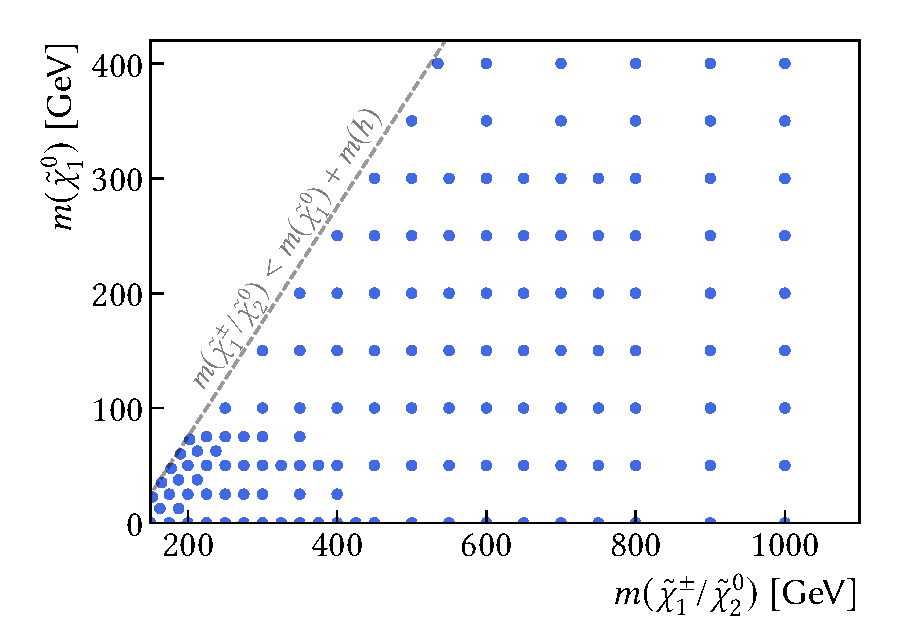
\includegraphics[width=0.5\textwidth]{signalgrid}}
%\end{figure}

In searches for BSM physics at the Large Hadron Collider, it is common to use simplified models~\cite{SimplifiedModels1:2008ag,SimplifiedModels2:2011wf,Alves:2011sq} as a way of reducing the available parameter space to a manageable level.
%Simplified models do not aim to represent complete supersymmetric models but are mostly defined by the empirical objects and kinematic variables used in the searches, typically allowing only a small number of sparticles to be involved in the decay chain (usually only two or three).
Simplified models do not aim to represent complete supersymmetric models but are mostly defined by a single (or a few selected) decay chain(s) allowing only a small number of sparticles, usually only two or three.
Other sparticles are decoupled by setting their masses to be kinematically inaccessible at current collider experiments. The decay chains of the participating sparticles are determined by fixed branching ratios, often set to be 100\%.
Experimental bounds from non-observation of a given model are then usually presented in function of the physical masses of the sparticles involved in the decay chain.
The model space spanned by the free parameters of the simplified model is typically called a \textit{signal grid}, as each set of distinct mass parameter values, called \textit{signal point}, occupies a single discrete point in this space. \Cref{fig:signalgrid} illustrates the signal grid used in \cref{part:simplified_model_analysis} of this thesis. The exact details of the signal grid are further discussed in \cref{sec:models_used}.
 
Simplified models have the inherent advantage that they circumvent the issue of having to search for SUSY in a vast parameter space where many of the parameters may only have small effects on observables. Their interpretation in terms of limits on individual SUSY production and decay topologies in function of sparticle masses is straightforward and very convenient.
The hope is, that simplified models are a reasonable approximation of sizeable regions of parameter space of the more complete model they are embedded in~\cite{pdg2020}. The obvious downside is however, that the limits obtained in simplified models are not automatically a good approximation of the true underlying constraint on the respective model parameter when interpreted in more complete SUSY models.
Often, the constraints set on sparticle masses in simplified models, significantly overestimate the true constraints obtained in more complex SUSY spectra, especially when the usual 100\% branching fractions are assumed in the simplified models (see \eg~\cite{Ambrogi:2017lov,Buchmueller:2013exa}).

One way of circumventing these issues, while sticking to the simplified model approach, is to ensure that the limits obtained in different simplified models involving different production and decay mechanisms are combined into limits representing more complex SUSY spectra.
In such an approach, the simplified model limits can be seen as building blocks for more realistic SUSY models that include many different production processes and decay modes.
Another possibility is to perform reinterpretations of SUSY searches---optimised for one ore more such simplified models---in more complete (and high-dimensional) SUSY model spaces, like \eg, in the \gls{pmssm}. This cannot only demonstrate the sensitivity of existing SUSY searches beyond simplified models, but also potentially identify blind spots and model regions not covered by current searches.
In addition, connections to (in)direct \gls{dm} searches and various \gls{sm} measurements can be explored this way. Recent efforts in this direction include, \eg, \references\cite{Ambrogi:2017lov, Aaboud:2016wna, pMSSM-scan-run1:2015baa}. As will be discussed in \cref{part:reinterpretation} of this thesis, efforts reinterpreting ATLAS searches for \gls{susy} In \cref{ch:pmssm}, a reinterpretation of the search for electroweakinos presented herein using a set of \gls{pmssm} models, is discussed.


\section{Search for electroweakinos}

\begin{figure}
	\centering
	\begin{subfigure}[b]{0.33\linewidth}
		\centering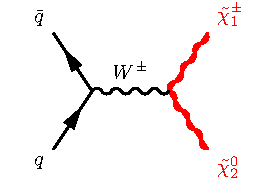
\includegraphics[width=.9\textwidth]{electroweakino_production_1}
		\caption{\label{fig:electroweakino_production_1}}
	\end{subfigure}%
	\begin{subfigure}[b]{0.33\linewidth}
		\centering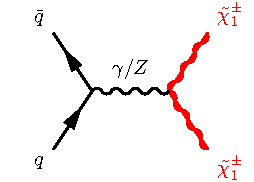
\includegraphics[width=.9\textwidth]{electroweakino_production_2}
		\caption{\label{fig:electroweakino_production_2}}
	\end{subfigure}%
	\begin{subfigure}[b]{0.33\linewidth}
		\centering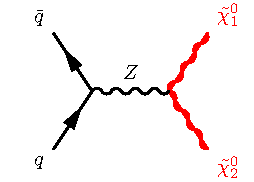
\includegraphics[width=.9\textwidth]{electroweakino_production_3}
		\caption{\label{fig:electroweakino_production_3}}
	\end{subfigure}	
	\caption{Dominant diagrams for production of electroweakino pairs at the Large Hadron Collider. Adapted from \reference\cite{Martin:1997ns}}\label{fig:electroweakino_production}
\end{figure}

While both the ATLAS experiment~\cite{ATLASsummary} and CMS experiment~\cite{CMSsummary} at the Large Hadron Collider at CERN set strong limits on the presence of gluinos and squarks at the TeV scale, the limits on electroweakinos are mostly still below $\SI{1}{\TeV}$. 
The reason for the relatively low limits on electroweakinos are the low cross-sections of electroweakino production, compared to those of squark and gluino production.
As can be seen in \cref{fig:SUSY_xsecs}, the cross sections for $\charg\neutr$ pair-production (the production process considered in the following, as discussed below) is more than two orders of magnitude smaller than that for gluino pair-production.  

Apart from the electroweakino mass limits set by the current collider experiments, some additional limits from the LEP experiments are still relevant in some corners of the phase space. Combining the results from all four LEP experiments leads to a general lower chargino mass limits of $\SI{103.5}{\GeV}$, except for scenarios with a low sneutrino mass~\cite{lep_susy_results}. For small mass splittings between the $\charg$ and the $\lsp$, the lower limit is a little weaker, with dedicated searches excluding charginos with $m(\charg) < \SI{91.9}{\GeV}$~\cite{lep_susy_results}. For mass splittings larger than $\SI{1.5}{\GeV}$ and up to $\SI{50}{\GeV}$, the \gls{lep} chargino limits have recently been superseded by a dedicated ATLAS search for compressed \gls{susy} scenarios~\cite{SUSY-2018-16}. For the neutralino, a general lower limit on the lightest neutralino mass comes from limits on the invisible width of the $Z$ boson, excluding $m(\lsp) < \SI{45.5}{\GeV}$\footnote{Depending on the coupling between the $Z$ boson and the lightest neutralino.}~\cite{pdg2020}. \improvement{displaced leptons}

\begin{figure}
\floatbox[{\capbeside\thisfloatsetup{capbesideposition={right,center},capbesidewidth=0.35\textwidth}}]{figure}[\FBwidth]
{\caption{Cross sections of different \gls{susy} production processes at $\sqrt{s}=\SI{13}{\TeV}$ in $pp$ collisions. Cross sections for pair-production of electroweakinos are significantly smaller than, \eg, those for pair-production of gluinos. The shaded bands correspond to the theory uncertainty of each cross section. Cross sections taken for coloured and electroweak sector taken from \references\cite{Beenakker:2016lwe,Beneke:2009ye} and \references\cite{Fiaschi:2018hgm,Fuks:2012qx,Fiaschi:2018xdm}, respectively.}\label{fig:SUSY_xsecs}}
{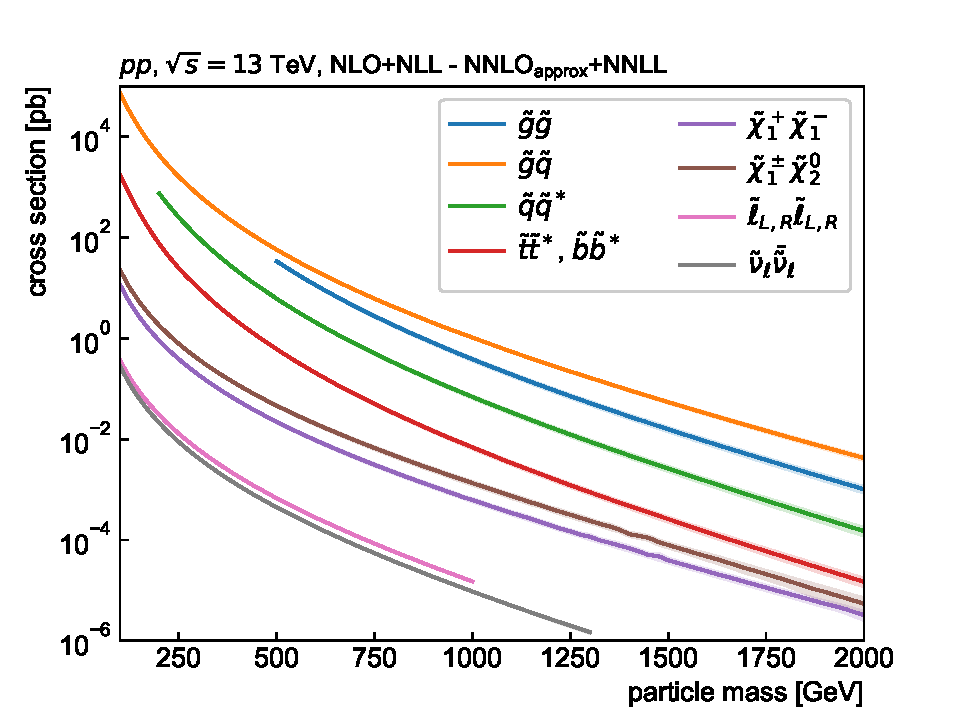
\includegraphics[width=0.6\textwidth]{SUSY_xsecs_v1}}
\end{figure}

\subsection{Production of electroweakinos at the Large Hadron Collider}

If gluinos and squarks are heavier than a few TeV, \ie too heavy to be within reach of the Large Hadron Collider, the direct production of electroweakinos might be the dominant production mode of SUSY. At hadron colliders, electroweakinos can be pair-produced directly via electroweak processes. The direct production of electroweakino pairs dominantly happens through electroweak gauge bosons from \textit{s}-channel $q\bar{q}$ annihilation, as shown in \cref{fig:electroweakino_production}. Contributions from \textit{t}-channels via squark exchange are typically of less importance~\cite{Martin:1997ns}.


\subsection{Models used within this work}\label{sec:models_used}

%\begin{figure}
%	\centering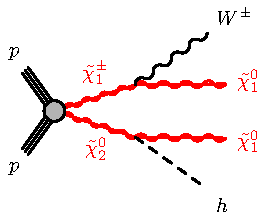
\includegraphics[width=.4\textwidth]{C1N2-WhN1N1}
%	\caption{Diagram for $\charg\neutr$ pair-production with subsequent decays into $\charg\rightarrow W^\pm\lsp$ and $\neutr\rightarrow h\lsp$.}\label{fig:Wh_model}
%\end{figure}

\begin{figure}
	\centering
	\begin{subfigure}[b]{0.45\linewidth}
		\centering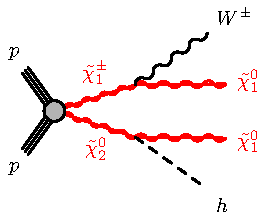
\includegraphics[width=.85\textwidth]{C1N2-WhN1N1}
		\caption{\label{fig:Wh_model}}
	\end{subfigure}%
	\begin{subfigure}[b]{0.55\linewidth}
		\centering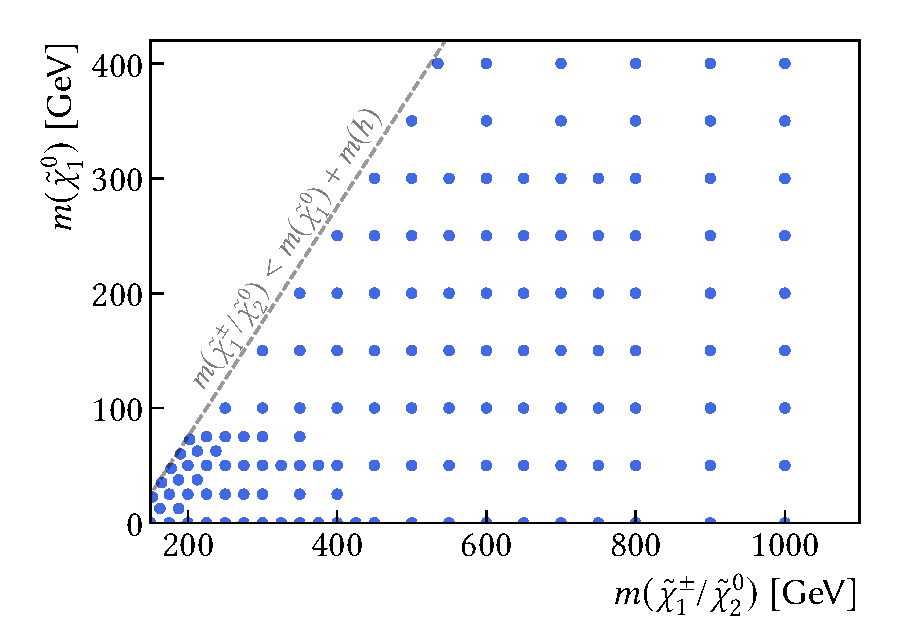
\includegraphics[width=.9\textwidth]{signalgrid}
		\caption{\label{fig:signalgrid}}
	\end{subfigure}	
	\caption{Simplified model used in this thesis. Fig.~\subref{fig:Wh_model} shows a diagram for $\charg\neutr$ pair-production with subsequent decays into $\charg\rightarrow W^\pm\lsp$ and $\neutr\rightarrow h\lsp$. Fig.~\subref{fig:signalgrid} shows the signal grid used. Each discrete point represents a different signal model with a unique set of $\charg/\neutr$ and $\lsp$ masses.}\label{fig:models_used}
\end{figure}

%\begin{figure}
%\floatbox[{\capbeside\thisfloatsetup{capbesideposition={right,center},capbesidewidth=0.4\textwidth}}]{figure}[\FBwidth]
%{\caption{Diagram for $\charg\neutr$ pair-production with subsequent decays into $\charg\rightarrow W^\pm\lsp$ and $\neutr\rightarrow h\lsp$.}\label{fig:Wh_model}}
%{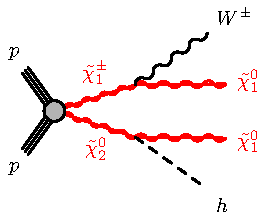
\includegraphics[width=0.5\textwidth]{C1N2-WhN1N1}}
%\end{figure}

In SUSY scenarios where the sleptons and charged and pseudoscalar Higgs bosons are heavier than the charginos and neutralinos, a relatively pure wino lightest chargino decays predominantly through $\charg\rightarrow W^\pm\lsp$, while the next-to-lightest neutralino decays via $\neutr\rightarrow Z/h\lsp$. If, in addition, the higgsinos are much heavier than the wino, and the mass splitting between the two lightest neutralinos is larger than the Higgs boson mass, the decay $\neutr\rightarrow h\lsp$ is the dominant decay mode of the $\neutr$. In this case, both the $\charg$ and $\neutr$ are wino-like and nearly mass-degenerate.

The main model used in the following is a simplified model considering direct production of a $\charg\neutr$ pair, where the lightest chargino decays via $\charg\rightarrow W^\pm\lsp$ and the next-to-lightest neutralino decays via $\neutr\rightarrow h\lsp$, each with 100\% branching ratio.
The lightest chargino $\charg$ and the next-to-lightest neutralino $\neutr$ are assumed to be degenerate in mass and pure wino states, while the lightest neutralino $\lsp$ is considered to be a pure bino \gls{lsp}.
The mass parameter hierarchy for this model is thus $\vert M_1 \vert < \vert M_2 \vert \ll \vert\mu\vert$. 

The masses of $\charg/\neutr$ and $\lsp$ are free parameters and are systematically varied, creating a two-dimensional signal grid to be scanned and compared to data. \Cref{fig:signalgrid} shows the two-dimensional signal grid used in \cref{part:simplified_model_analysis} of this thesis. In the simplified model, the Higgs boson mass is set to $\SI{125}{\GeV}$ in accordance with the measured value~\cite{Aad:2012tfa,Chatrchyan:2012ufa} and its branching ratios are the ones from the \gls{sm}. An exemplary diagram for the simplified model considered is shown in \cref{fig:Wh_model}.

In addition to the simplified model targeted by the SUSY search presented in the following, an additional class of models is considered in the second part of this work. These models are sampled directly from the \gls{pmssm} parameter space and are used to reinterpret the aforementioned search for direct pair-production of electroweakinos. The mass spectrum of an exemplary \gls{pmssm} model point used is shown in \cref{fig:slha}. Additional details on the sampling of the \gls{pmssm} models are given in~\cref{sec:pmssm_sampling}. 


\begin{figure}
	\centering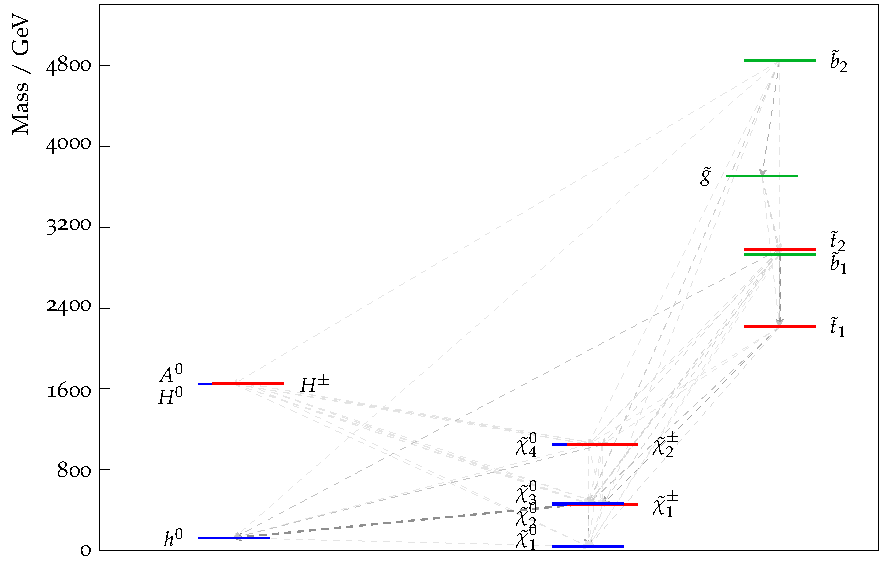
\includegraphics[width=.8\textwidth]{slha}
	\caption{Mass spectrum of an example \gls{pmssm} model point considered in \cref{part:reinterpretation} of this thesis. The kinematically allowed decays and their branching ratios are indicated through dashed lines. Figure generated using \texttt{pyslha}~\cite{pyslha:2013jua}.}\label{fig:slha}
\end{figure}

%\begin{figure}
%\floatbox[{\capbeside\thisfloatsetup{capbesideposition={right,center},capbesidewidth=0.4\textwidth}}]{figure}[\FBwidth]
%{\caption{Diagram for $\charg\neutr$ pair-production with subsequent decays into $\charg\rightarrow W^\pm\lsp$ and $\neutr\rightarrow h\lsp$.}\label{fig:slha}}
%{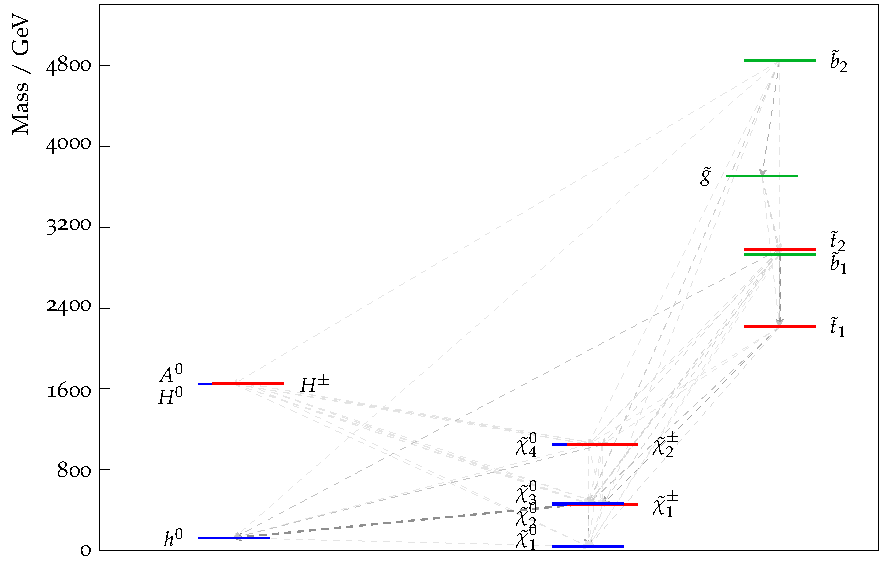
\includegraphics[width=0.5\textwidth]{slha}}
%\end{figure}




%!TEX root = ../thesis.tex
%*******************************************************************************
%*********************************** Experiment *****************************
%*******************************************************************************

\chapter{Experiment} 

\ifpdf
    \graphicspath{{chapter-experiment/Figs/Raster/}{chapter-experiment/Figs/PDF/}{chapter-experiment/Figs/}}
\else
    \graphicspath{{chapter-experiment/Figs/Vector/}{chapter-experiment/Figs/}}
\fi


One of Europe's first joint ventures in science~\cite{About:1997225}, CERN (Conseil Européen pour la Recherche Nucléaire) is the largest physics research facility in the world, bringing together more than \num[group-separator={,}]{12200} people from of 110 nationalities to work together and push the frontiers of science and technology. Located at the Franco-Swiss border near Geneva, CERN was founded in 1954 and nowadays counts 23 member states~\cite{About:1997225}. CERN's main research area is particle physics, hence why the organization operates a full complex of particle accelerators and detectors.

This chapter introduces the \gls{lhc}, CERN's main particle accelerator, as well as the ATLAS experiment, in which the \gls{susy} search presented in this work is embedded in.

\section{The Large Hadron Collider}\label{sec:lhc}

The LHC~\cite{Evans:1129806} is the largest particle accelerator situated at CERN. It is installed in a tunnel with $\SI{26.7}{\km}$ circumference, that was originally constructed from 1984 to 1989 for the \gls{lep} accelerator. The tunnel is situated on the Franco-Swiss border and wedged between the Jura mountains and lake Léman. It lies between $\SI{45}{\meter}$ (in the limestone of the Juar) and $\SI{170}{\meter}$ (in molasse rock) below the surface, resulting in a tilt of $1.4\%$ towards the lake.  While proton-proton ($pp$) collisions are the main operating mode of the \gls{lhc}, its design also allows it to accelerate and collide heavy ions like lead and xenon. Since data from $pp$ collisions is used in this work, the following sections will mainly focus on this operating mode. As a particle-particle collider, the \gls{lhc} obviously consists of two rings with counter-rotating beams, as opposed to particle-antiparticle colliders that only need a single ring. With an inner diameter of only $\SI{3.7}{\meter}$, the tunnel however simply too narrow to fit two separate proton rings. Instead the \gls{lhc} is built in a twin bore design\footnote{Originally proposed by John Blewett at BNL for cost-saving measures of the Colliding Beam Accelerator~\cite{Evans:1129806}.}, housing two sets of coils and beam channels in a single magnetic and mechanical structure and cryostat~\cite{Evans:1129806}. While saving costs, this design has the disadvantage of both beams being magnetically coupled, thereby reducing flexibility of the machine. 

Before being injected into the LHC, protons are pre-accelerated by an injection chain built from multiple existing machines in CERN's accelerator complex, pictured in \cref{fig:accelerator_complex}. The injection chain consists of predecessor accelerators that have been upgraded in order to be able to handle the high luminosity and high energy requirements of the \gls{lhc}. The protons for the \gls{lhc} stem from a duoplasmatron source~\cite{Scrivens:1382102}, stripping electrons from hydrogen atoms through electric discharges between a hot anode and cathode. The $\SI{90}{\keV}$ protons are then accelerated by a \gls{rf} quadrupole to $\SI{750}{\keV}$ before being injected into Linac2\footnote{Originally built to replace Linac 1 in order to produce higher energetic proton beams, Linac 2 has been replaced by Linac 4 in 2020.}, a linear accelerator producing a beam of $\SI{50}{\MeV}$ protons through the use of \gls{rf} cavities. The protons then enter a set of circular accelerators, the Proton Synchrotron Booster (PSB), the \gls{ps} and the \gls{sps}, creating a stepwise acceleration up to an energy of $\SI{450}{\GeV}$, which is the injection energy of the \gls{lhc}. The \gls{lhc} finally accelerates the protons up to nominal beam energy before colliding them. 

\begin{figure}
	\centering    
	\includegraphics[width=0.9\textwidth]{CCC-v2019-final-white}
	\caption[CERN accelerator complex]{CERN accelerator complex as of 2018~\cite{Mobs:2684277}.}
	\label{fig:accelerator_complex}
\end{figure}

The \gls{lhc} is composed of eight straight sections and eight arcs. The eight straight sections each serve as interaction points (\textit{Point}), either for particle detectors, or for machine hardware of the collider itself. The Points are labelled clockwise, with IP 1 being closest to the CERN Meyrin site. Four of the eight Points house the main particle physics experiments at the LHC, called ATLAS, CMS, ALICE and LHCb, covering a wide range of fundamental research. The two general purpose particle detectors ATLAS~\cite{Aad:2008zzm} and CMS~\cite{Chatrchyan:2008aa} are installed at Point~1 and Point~5, respectively. Both ATLAS and CMS are designed to perform high precision SM measurements including Higgs measurements as well as searches for BSM physics. Being very similar in terms of targeted phase space, ATLAS and CMS can be used to cross-check results of each other. ALICE~\cite{Aamodt:2008zz} is situated at Point~2 and specializes on heavy ion physics, studying the physics of quark-gluon plasma at high energy densities. Built in Point~8, LHCb~\cite{Alves:2008zz} targets $B$-physics and performs measurements of CP-violation. Apart from the four main experiments, three smaller experiments exist at the \gls{lhc}: TOTEM, MoEDAL and LHCf. While TOTEM~\cite{Anelli:2008zza} and LHCf~\cite{Adriani:2006jd} study forwards physics close to CMS and ATLAS, respectively, MoEDAL~\cite{Pinfold:2009oia} searches for magnetic monopoles.

The remaining four Points house accelerator equipment needed for operation of the LHC. Most of the collimation system is placed at Point~3 and Point~7, performing beam cleaning and machine protection through a series of beam intercepting devices, ensuring that no stray particles from experimental debris or beam halo can reach and damage other machine components. The acceleration of the beam itself is performed at Point~4 with two \gls{rf} systems, one for each \gls{lhc} beam. The \gls{rf} cavities operate at $\SI{400}{\MHz}$ and provide $\SI{8}{MV}$ during injection and $\SI{16}{MV}$ during coast~\cite{Evans:1129806}. Due to the \gls{rf} acceleration, the accelerated protons are grouped in packages called \textit{bunches}, each containing roughly $10^{11}$ protons, with a bunch spacing of $\SI{25}{ns}$~\cite{Evans:1129806}. Each beam contains a total of 2808~\cite{Evans:1129806} bunches as design value. The remaining Point~6 houses the beam dumping system, allowing to horizontally deflect and fan out both beams into dump absorbers using fast-paced \textit{kicker} magnets. The two nitrogen-cooled dump absorbers each consist of a graphite core contained in a steel cylinder, surrounded by $\SI{750}{\tonne}$ of concrete and iron shielding~\cite{Bruning:782076}. Insertion of the beams from the SPS into the \gls{lhc} happens at Points~2 and 8, close to the ALICE and LHCb experiments.

The eight arcs of the \gls{lhc} are filled with dipole magnets built from superconducting NbTi Rutherford cables. The electromagnets are responsible for keeping the accelerated particles on their circular trajectory and are the limiting factor of the maximal centre-of-mass energy $\sqrt{s}$ of the \gls{lhc}. In order to achieve the design energy of $\sqrt{s} = \SI{14}{\TeV}$~\cite{Bruning:782076}, the magnets have to create a field strength of $\SI{8.3}{T}$~\cite{Evans:1129806}. In order to sustain the electric currents needed for such high field strengths, the magnets need to be cooled down to $\SI{1.9}{K}$~\cite{Evans:1129806} using superfluid helium and operated in superconducting state. In addition to the dipole magnets, the arcs contain quadrupole magnets used to shape and focus the beams, as well as multipole magnets correcting and optimizing the beam trajectory. Quadrupole magnets are also used to reduce the beam size before and after the interaction points.

\subsection{Pileup}

\begin{figure}
	\centering
	\begin{subfigure}[b]{0.45\linewidth}
		\centering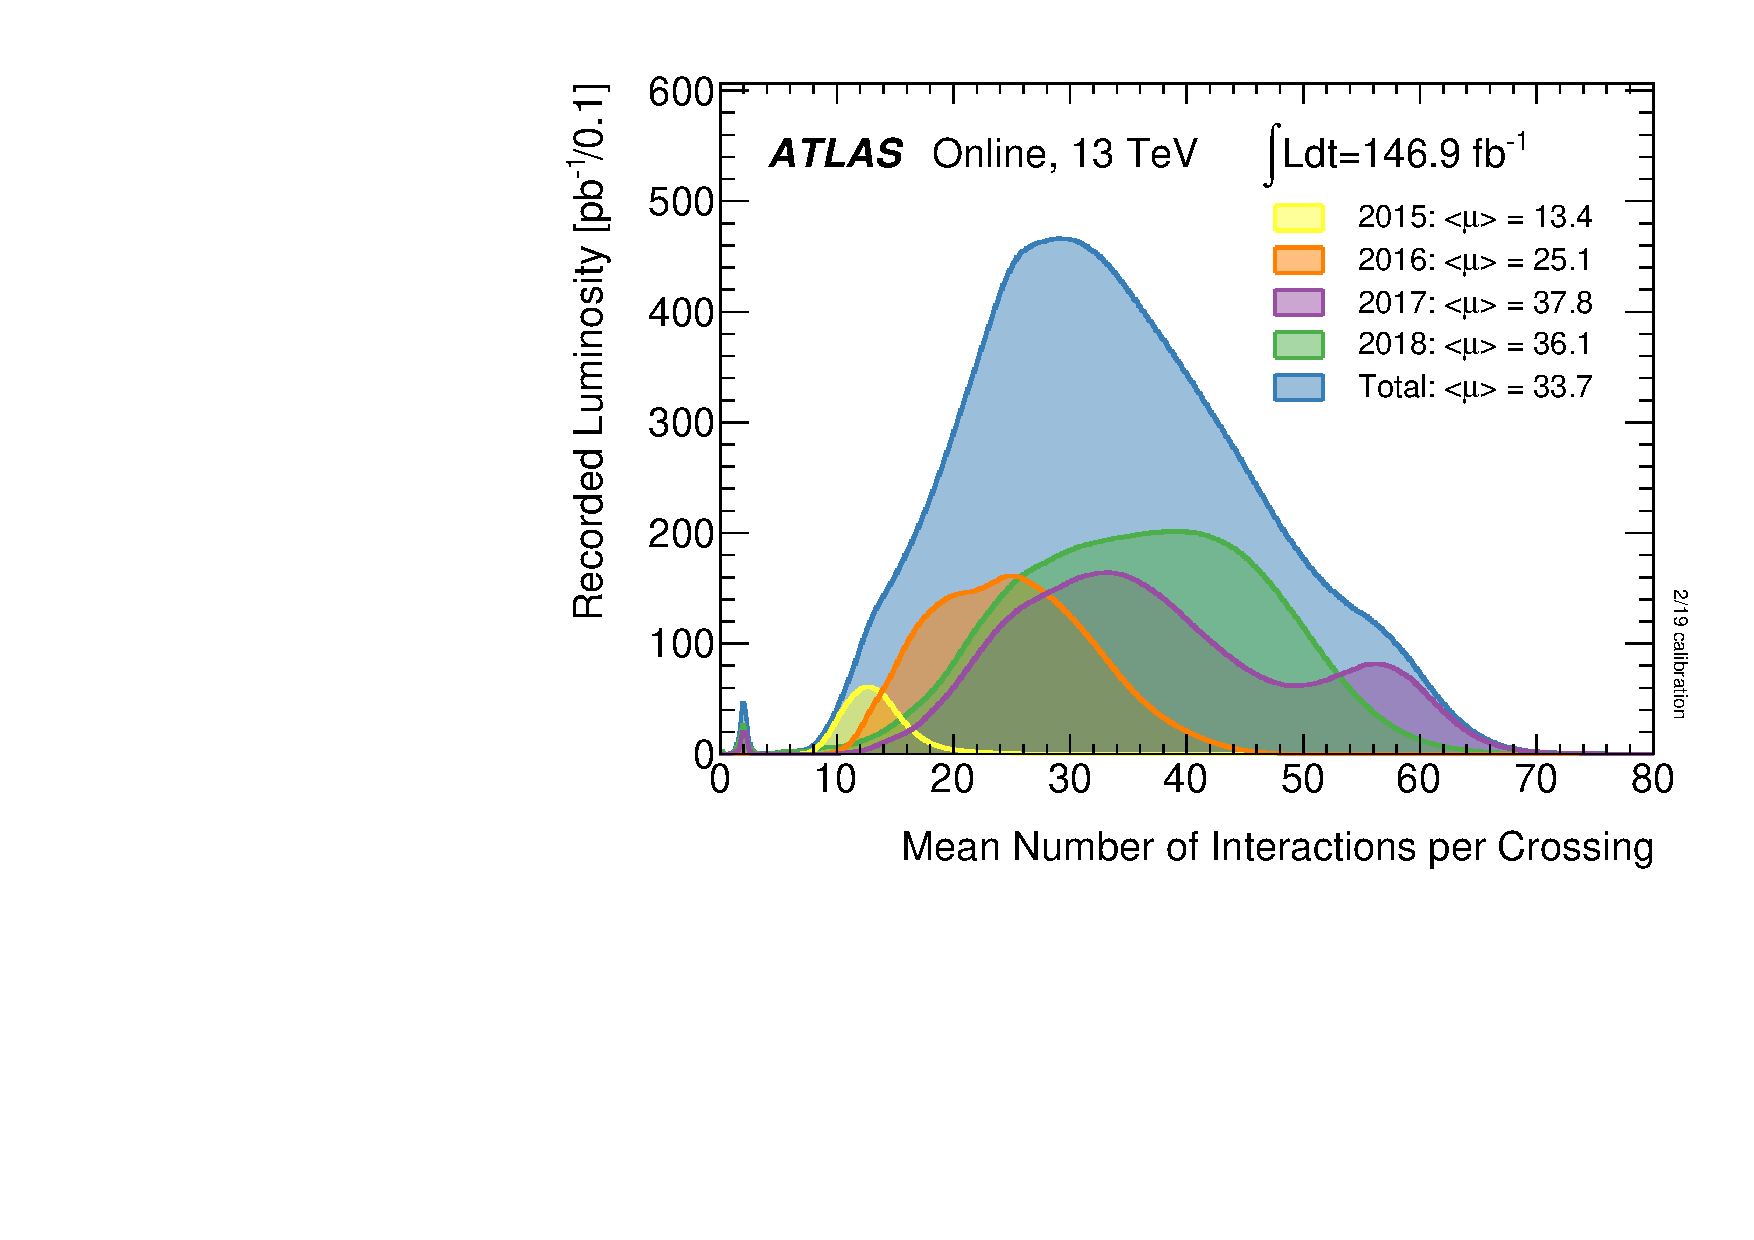
\includegraphics[width=\textwidth]{mu_2015_2018}
		\caption{Luminosity-weighted mean number of interactions per bunch crossing during Run~2 data-taking.\label{fig:mu_2015_2018}}
	\end{subfigure}%
	\begin{subfigure}[b]{0.45\linewidth}
		\centering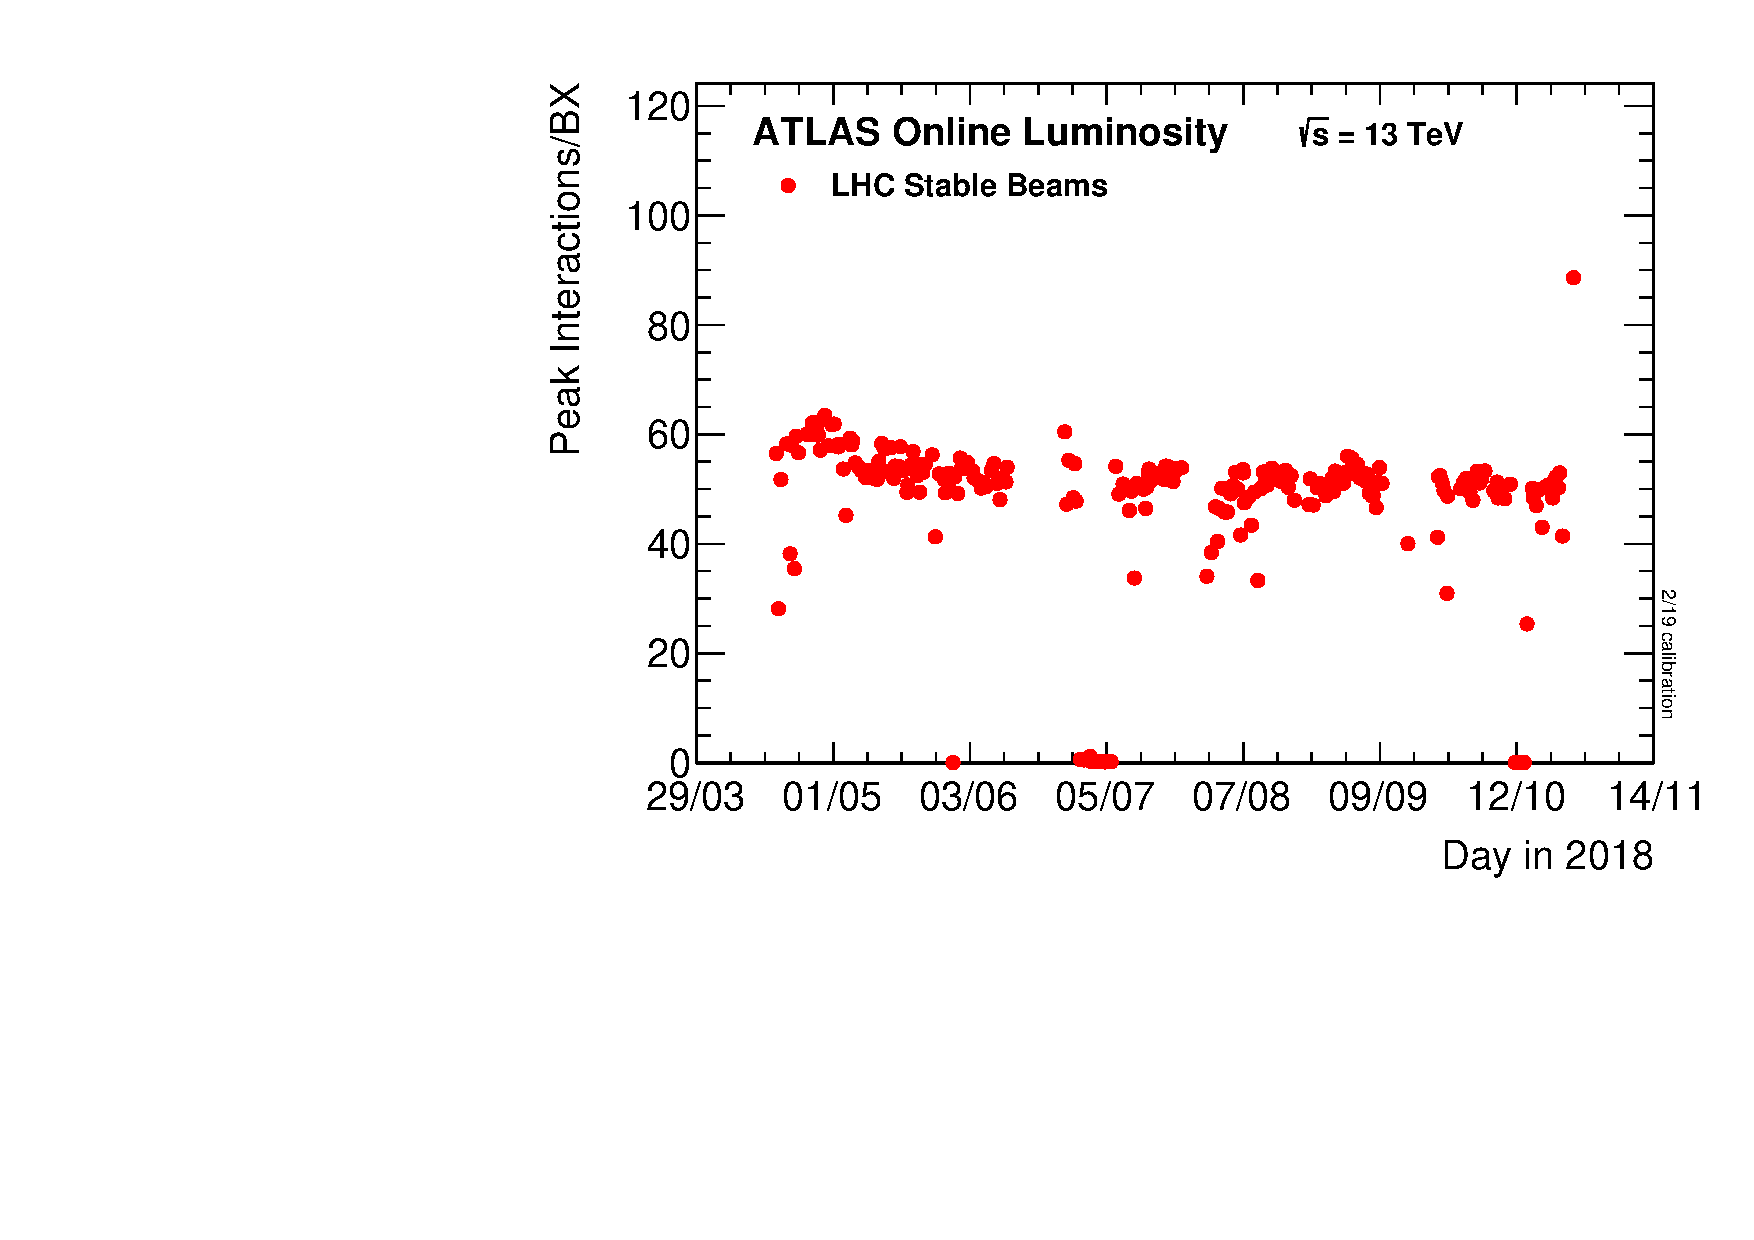
\includegraphics[width=\textwidth]{peakMuByFill}
		\caption{Peak mean number of interactions per bunch crossing for each fill during 2018.\label{fig:peakMuByFill}}
	\end{subfigure}%
	\caption{Number of interactions per bunch crossing recorded by the ATLAS detector~\cite{ATLAS:Run2}}\label{fig:mu_run2}
\end{figure}

Due to the high number of protons in each bunch, several $pp$ collisions occur at each bunch crossing. This leads to a phenomenon called \textit{pile-up}, where the recorded events not only contain information from the hard-scattering process of interest, but also remnants from additional, often low-energy, $pp$ collisions. During the Run~2 data-taking period, the mean number of inelastic $pp$ collisions per bunch crossing, $\mu$, has varied from roughly 10 to 70, with the majority of bunch crossings having a value of $\mu$ around 30. \Cref{fig:mu_2015_2018} shows the mean number of interactions per bunch crossing during the Run~2 data-taking period, weighted by luminosity. The peak number of interactions per bunch crossing $\mu_\mathrm{peak}$ per fill has been consistently around 50 during the 2018 data-taking (cf.~\cref{fig:peakMuByFill}).

Experimentally, pile-up can be divided into five major components~\cite{Marshall:2014mza}:
\begin{itemize}
	\item \textit{In-time} pile-up: multiple interactions during a single bunch crossing, of which not all will be interesting, as often with relatively low energy. If they can be resolved, the main hard-scattering event can still be isolated and studied.
	\item \textit{Out-of-time} pile-up: additional collisions occurring in bunch crossings before or after the main event of interest. This happens either due to read-out electronic integrating over longer time frames than the $\SI{25}{ns}$ bunch spacing, or detector components being sensitive to several bunch crossings.
	\item \textit{Cavern background}: gas of thermal neutrons and photons that typically fill the experimental caverns during a run of the LHC and tend to cause random hits in detector components.
	\item \textit{Beam halo events}: protons scraping an up-stream collimator, typically resulting in muons travelling parallel to the beam pip
	\item Beam gas events: collision events that originate from interactions between proton bunches and residual gas inside the beam pipe.
\end{itemize}
While the effects of cavern background can be mitigated through special pieces of shielding, beam halo and beam gas events leave signatures that can be recognized and removed. Signals from in-time and out-of-time pile-up create irreducible overlap with the events of interest, significantly impacting analyses, and thus need to be simulated~\cite{Marshall:2014mza}.

\subsection{Luminosity and data-taking}

\begin{figure}
	\centering
	\begin{subfigure}[b]{0.45\linewidth}
		\centering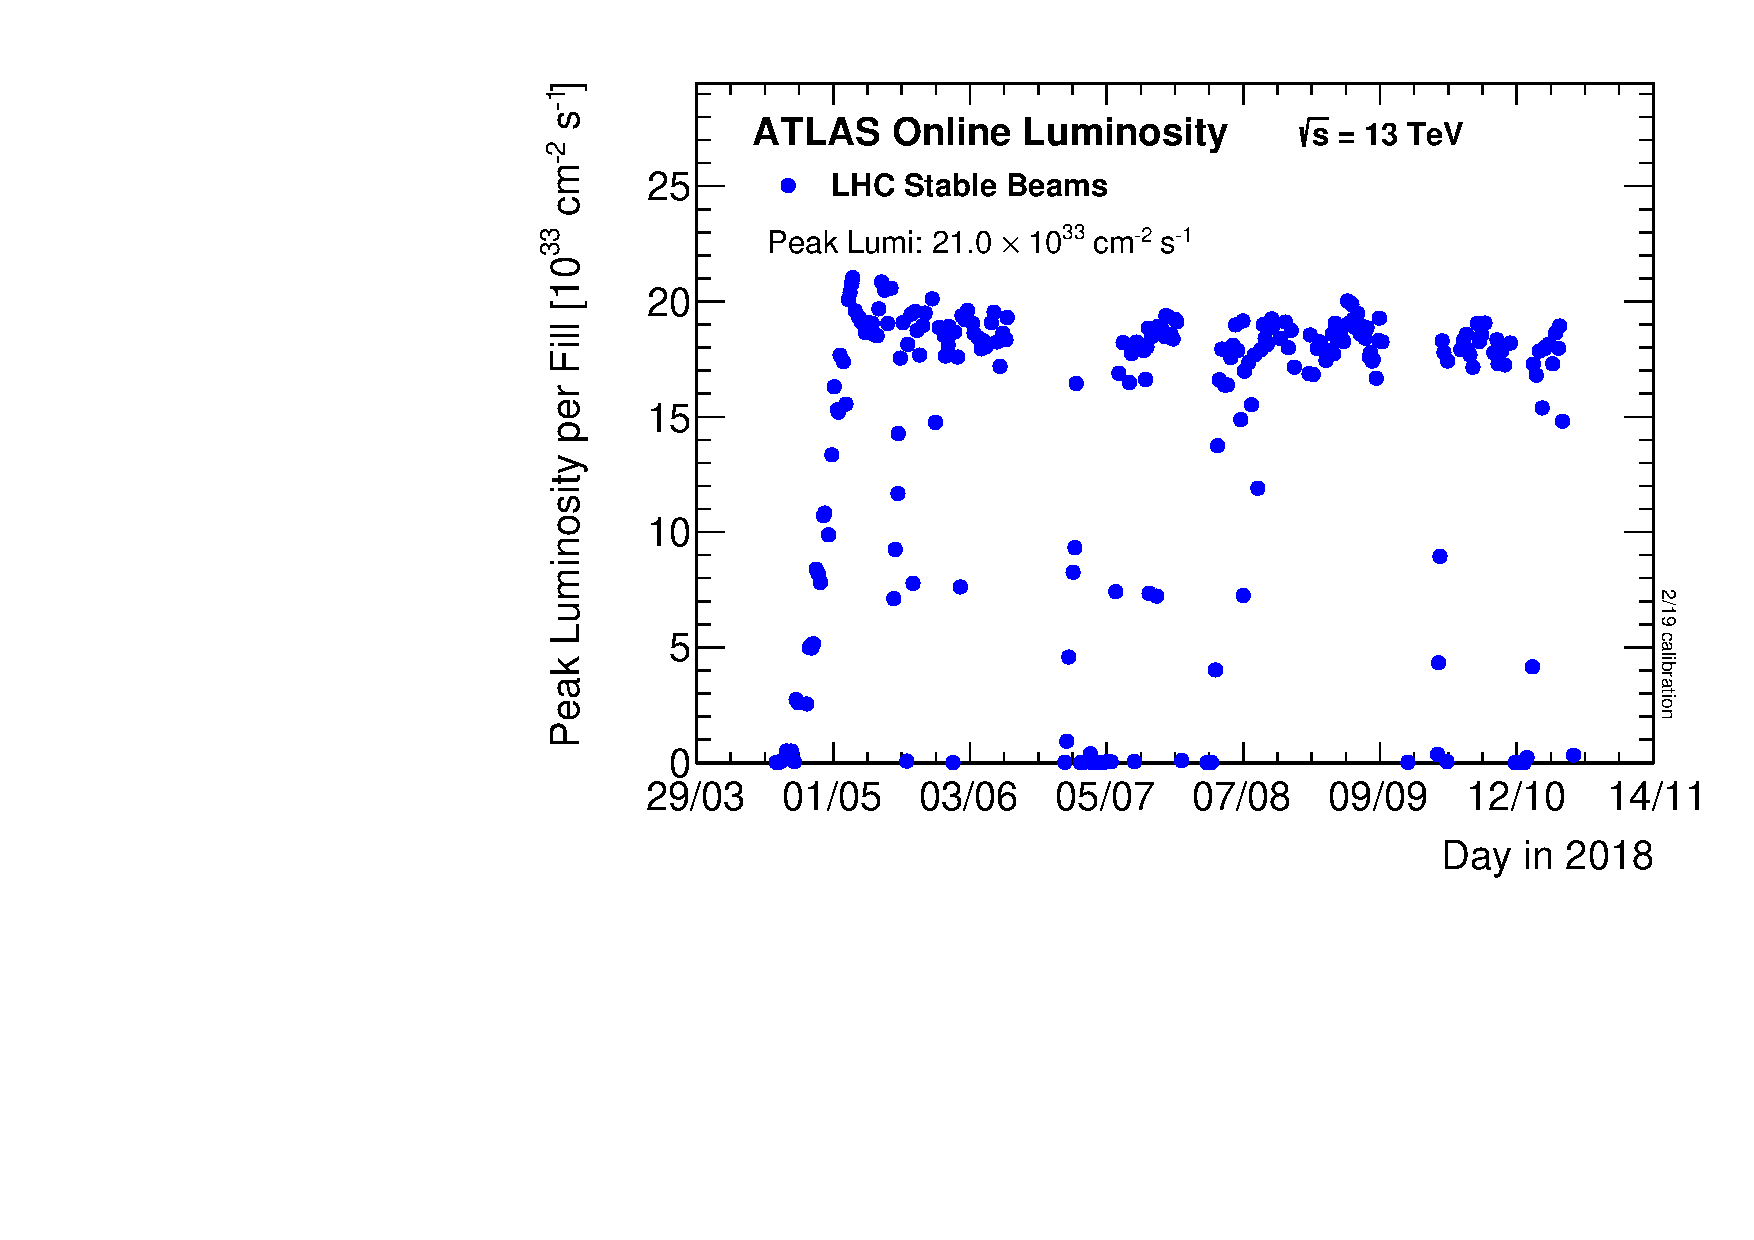
\includegraphics[width=\textwidth]{peakLumiByFill}
		\caption{\label{fig:peakLumiByFill}}
	\end{subfigure}%
	\begin{subfigure}[b]{0.45\linewidth}
		\centering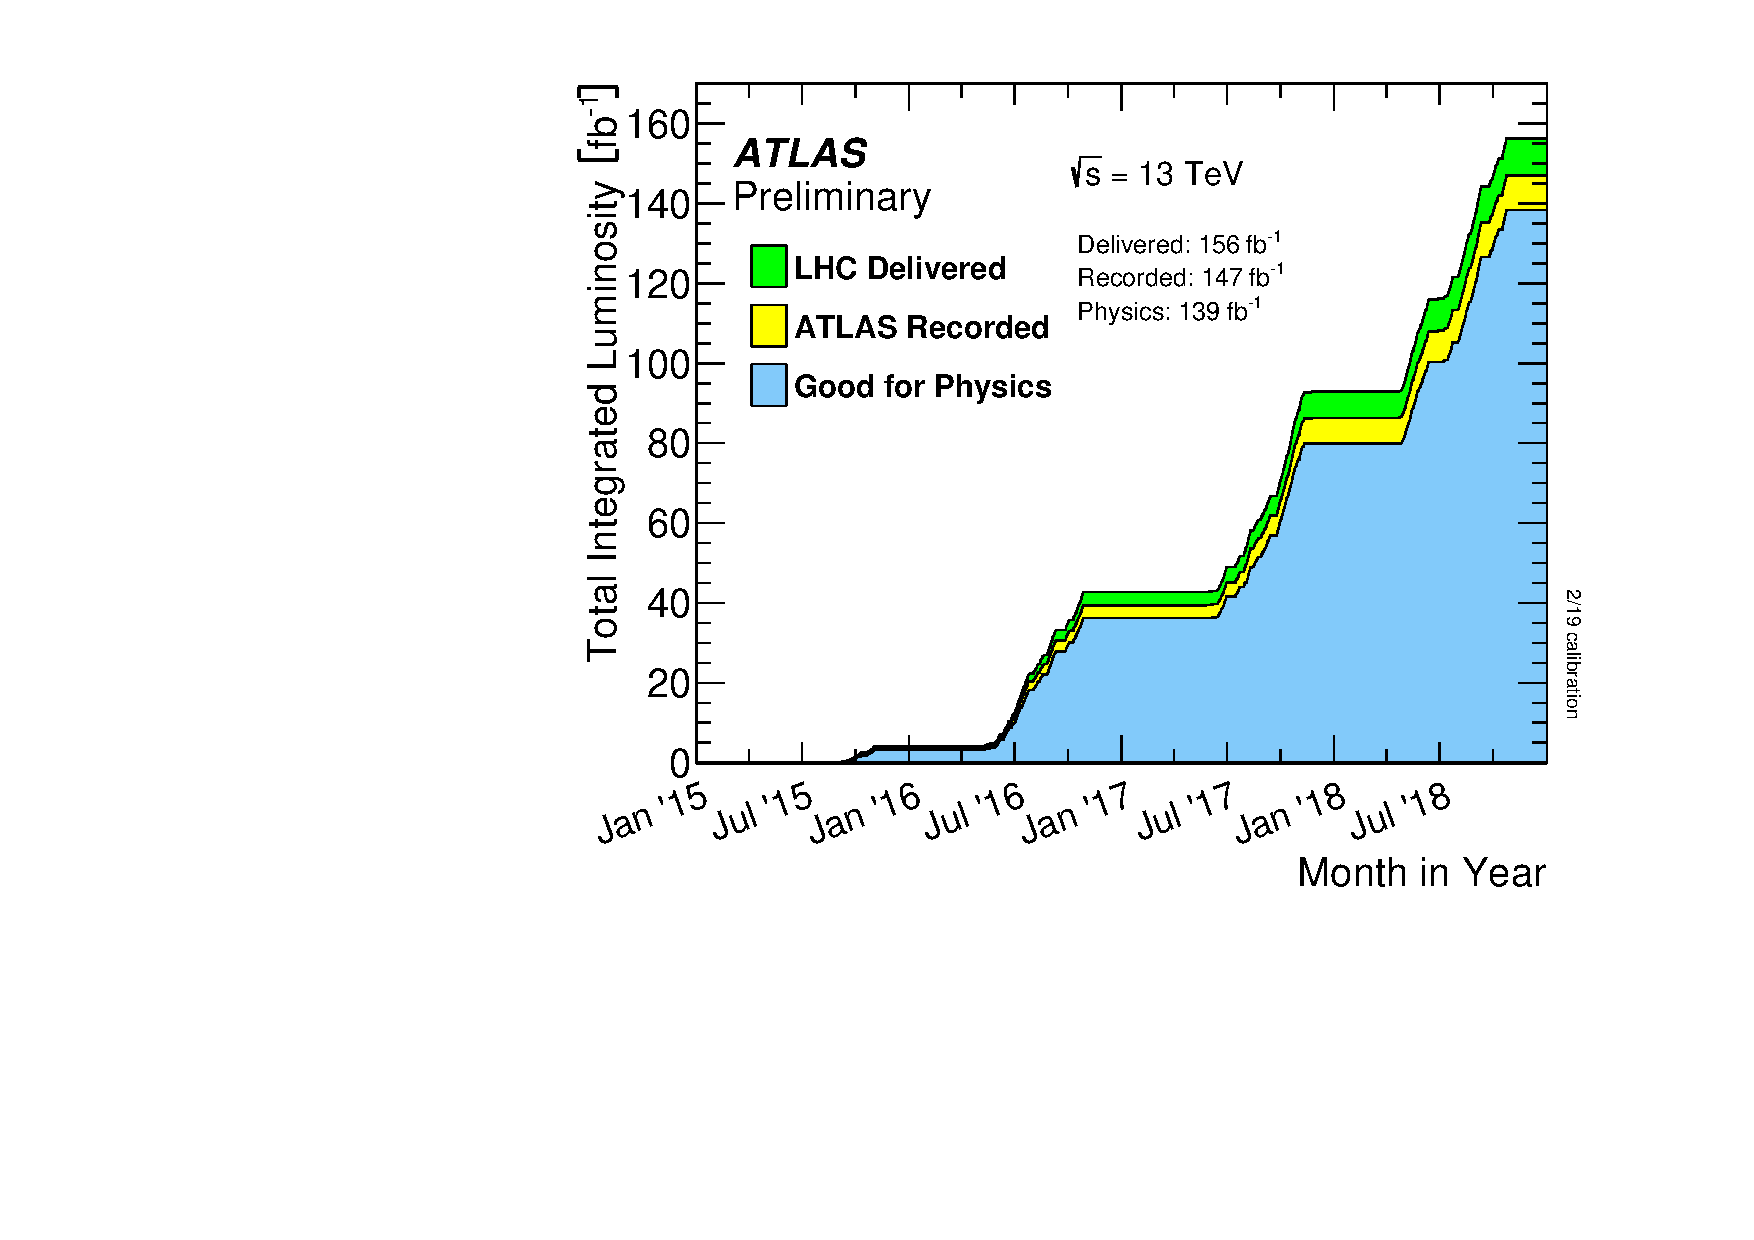
\includegraphics[width=\textwidth]{intlumivstimeRun2DQall}
		\caption{\label{fig:intlumivstimeRun2DQall}}
	\end{subfigure}%
	\caption{Instantaneous and cumulative luminosities in Run~2. Figure~\subref{fig:peakLumiByFill} shows the peak instantaneous luminosity delivered to ATLAS during $pp$ collision data taking in 2018 as a function of time. Figure~\subref{fig:intlumivstimeRun2DQall} shows the cumulative luminosity delivered to ATLAS (green), recorded by ATLAS (yellow) and deemed good for physics analysis (blue) during the entirety of Run~2~\cite{ATLAS:Run2}.}\label{fig:lumi_run2}
\end{figure}

Apart from the beam energy, the most important quantity for a collider is the instantaneous luminosity $L$. For a synchrotron with Gaussian beam distribution, the instantaneous luminosity can be written as
\begin{equation}
	L = \frac{N_b^2 n_b f_\mathrm{rev}}{4\pi\sigma_x\sigma_y} F,
	\label{eq:lumi}
\end{equation}
where $n_b$ is the number of bunches, $N_b$ the number of protons per bunch, $f_\mathrm{rev}$ the revolution frequency and $\sigma_x$ and $\sigma_y$ the transverse beam sizes. The parameters $F$ is a geometrical correction factor accounting for the reduction in instantaneous luminosity due to the beams crossing at a certain crossing angle. While the design instantaneous luminosity of the \gls{lhc} at the high-luminosity experiments ATLAS and CMS is $L = \SI{e34}{\per\cm\squared\per\second}$~\cite{Evans:1129806}, the 2017 and 2018 data-taking periods saw a peak luminosity twice as high~\cite{peak_lumi}.

The instantaneous luminosity is related to the total number of events $N$ through the cross section $\sigma$ of the events in question
\begin{equation}
	N = \sigma L_\mathrm{int} = \sigma \int L\diff t,
\end{equation}
with $L_\mathrm{int}$ the total integrated luminosity, a measure for the total amount of collision data produced.

A precise knowledge of the integrated luminosity corresponding to a given dataset is crucial for both SM measurements as well as searches for \gls{bsm} physics. Searches for \gls{susy} like the one presented in this work rely on precise measurements of the integrated luminosity in order to be able to estimate the contribution from SM background processes. The luminosity measurement for the Run~2 dataset used within this work is described in detail in~\cite{ATLAS-CONF-2019-021,Aaboud:2016hhf} and relies on a measurement of the bunch luminosity, \ie the luminosity produced by a single pair of colliding bunches
\begin{equation}
	L_b = \frac{\mu f_\mathrm{rev}}{	\sigma_\mathrm{inel}} = \frac{\mu_\mathrm{vis}f_\mathrm{rev}}{\sigma_\mathrm{vis}},
\end{equation}
with $\mu$ the pile-up parameter, $\sigma_\mathrm{inel}$ the cross section of inelastic $pp$ collisions, $\mu_\mathrm{vis} = \epsilon \mu$ is the fraction $\epsilon$ of the pile-up parameter $\mu$ visible to the detector and $\sigma_\mathrm{vis} = \epsilon\sigma_\mathrm{inel}$ the visible inelastic cross section. If $\sigma_\mathrm{vis}$ is known, the currently recorded luminosity can be determined by measuring $\mu_\mathrm{vis}$. At the ATLAS experiment, the observed number of inelastic interactions per bunch crossing $\mu\mathrm{vis}$ is measured using dedicated detectors, as for example LUCID-2~\cite{Avoni_2018}, a forward Cherenkov-detector using the quartz windows from photomultipliers as Cherenkov medium.
In order to use $\mu_\mathrm{vis}$ as luminosity monitor, the respective detectors need to be calibrated through a measurement of the visible inelastic cross section $\sigma_\mathrm{vis}$. This can be done using \gls{vdm} scans~\cite{vanderMeer:296752,GRAFSTROM201597}, in which the transverse distribution of protons in the bunches is inferred by measuring the relative interaction rates as a function of the transverse beam separation\footnote{Often called \textit{beam sweeping}.}. The algorithms used to determine the $\sigma_\mathrm{vis}$ calibration are described in~\cite{ATLAS-CONF-2019-021,Aaboud:2016hhf} and the luminosity during the \gls{vdm} runs can be determined using~\cref{eq:lumi}. At the \gls{lhc}, \gls{vdm} scans are typically performed in special low-$\mu$ runs with well-known machine parameters in order to minimise uncertainties~\cite{ATLAS-CONF-2019-021}. During high-$\mu$ physics runs, the luminosity measurement is then an extrapolation from the \gls{vdm} runs.

The \gls{lhc} entered operation in 2008, with first beams in September and first collisions by the end of November that same year~\cite{startup}. Its operation is in general structured into so-called \textit{Runs}, that are spanned by multiple years of data-taking. Run~1 spanned from 2009 to 2013 and delivered roughly $\SI{28.5}{\per\femto\barn}$ of $pp$ collision data to ATLAS, taken at centre-of-mass energies of $\SI{7}{\TeV}$ and $\SI{8}{\TeV}$~\cite{Aad:2011dr,Aad:1517411,Aaboud:2016hhf}. Run~2 lasted from 2015 to 2018 and saw a centre-of-mass energy increase to $\SI{13}{\TeV}$, delivering approximately $\SI{156}{\per\femto\barn}$ of $pp$ collision data to ATLAS~\cite{ATLAS-CONF-2019-021}. Run~3 of $pp$ collision data taking with two times design peak luminosity is currently planned to start its physics program in 2022 and last until end of 2024~\cite{run3}. Current plans foresee Run~3 to deliver about $\SI{150}{\per\femto\barn}$ of $pp$ collision data with centre-of-mass energies of $\SI{13}{\TeV}$ and $\SI{14}{\TeV}$. After Run~3, the \gls{lhc} will be upgraded to the High Luminosity \gls{lhc}, significantly increasing the peak instantaneous luminosity and delivering up to $\SI{3000}{\per\femto\barn}$ of $pp$ collision data from 2027 until 2040~\cite{run3,Apollinari:2284929}. 

This work uses $pp$ collision data taken by ATLAS during Run~2 of the \gls{lhc}. Of the $\SI{156}{\per\femto\barn}$ delivered to ATLAS, $\SI{147}{\per\femto\barn}$ were recorded, and $\SI{139}{\per\femto\barn}$ were deemed to be good for physics analysis. \Cref{fig:lumi_run2} shows the cumulative luminosity delivered to ATLAS during Run~2. Uncertainties on the measurement total recorded luminosity stem from the measurements of $\mu_\mathrm{vis}$ and $\sigma_\mathrm{vis}$, but are dominated by the uncertainties on $\sigma_\mathrm{vis}$ as \gls{vdm} scans can only be done during special runs, while the general conditions during high-$\mu$ conditions change continuously. For the full Run~2 dataset, the uncertainties accumulate to $\pm 1.7 \%$~\cite{ATLAS-CONF-2019-021}.

\section{ATLAS Experiment}\label{sec:atlas_experiment}

The ATLAS experiment is one of two general-purpose detectors at the LHC. Located at Point~1 in a cavern $\SI{100}{\meter}$ below the surface, it is approximately $\SI{44}{\meter}$ long and $\SI{25}{\meter}$ high~\cite{Aad:2008zzm}. The design of the ATLAS experiment is driven by the aim to allow for a diverse research program, including SM precision measurements, Higgs physics and searches for \gls{bsm} physics, whilst at the same time taking into account the unique and challenging conditions set by the \gls{lhc}. The various detector technologies used are designed to withstand the high-radiation environment of the \gls{lhc}, while allowing particle measurements with high spatial and temporal granularity. The general structure of ATLAS is depicted in \cref{fig:atlas_detector}, and consists of a central part, called \textit{barrel}, that has a cylindrical shape around the beam pipe, and two discs, called \textit{end-caps}, that close off the barrel on each side. This makes the ATLAS detector forward-backward symmetric and covering nearly the full solid angle of $4\pi$, which is needed in order to measure momentum imbalances caused by particles that only interact weakly with the detector material.

The interface between the ATLAS experiment and the \gls{lhc} is the beam pipe. In order to be maximally transparent to the particles created in the collisions, but also be able to withstand the forces from the vacuum, the beam pipe is made out of Beryllium close to the \gls{ip}, and stainless-steel further away from the \gls{ip}~\cite{Brock:1354959}.

The following sections introduce the working principles of the different detector components used in ATLAS, starting with the innermost component closest to the \gls{ip}, the inner detector, followed by the calorimeters in the middle and finally the muon spectrometers on the outside. If not otherwise stated, details on the detector components are extracted from~\cite{Aad:2008zzm}.

\begin{figure}
	\centering    
	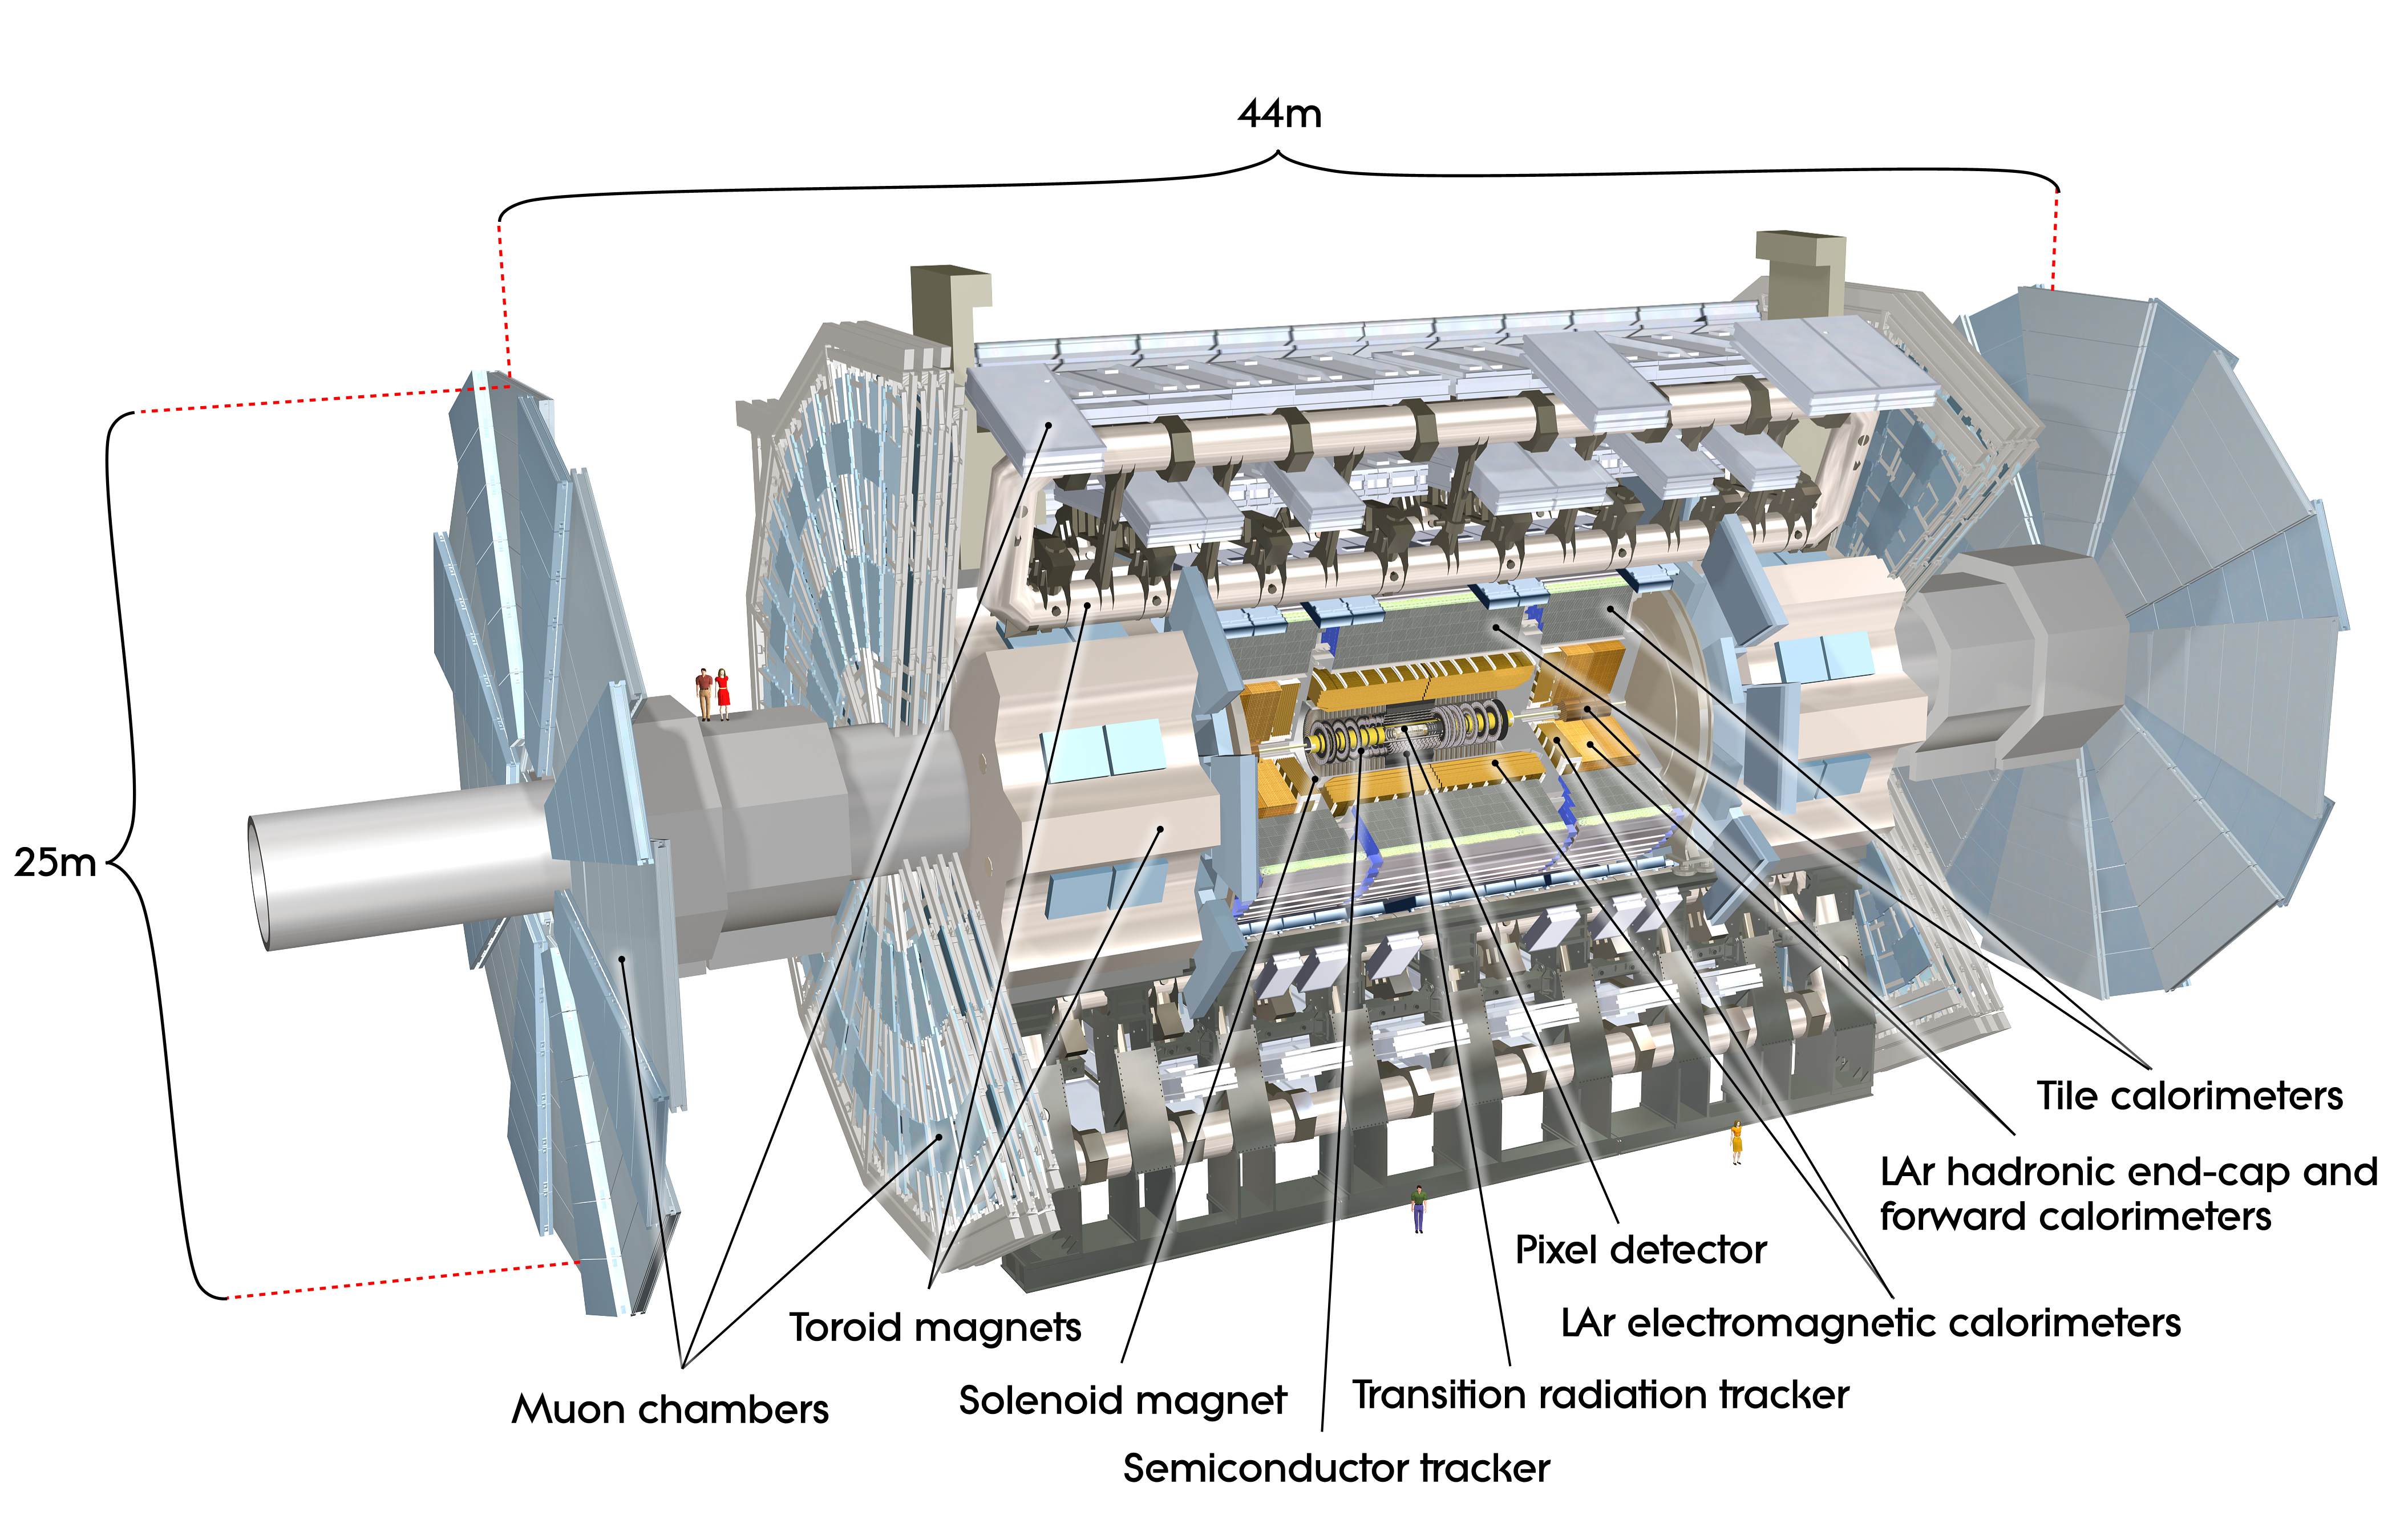
\includegraphics[width=0.9\textwidth]{atlas}
	\caption[The ATLAS detector]{Computer generated picture of the ATLAS detector, giving an overview on the various subsystems~\cite{Pequenao:1095924}.}
	\label{fig:atlas_detector}
\end{figure}


\subsection{Coordinate system}

In order to properly describe collision events in the ATLAS detector, a suitable detector system is needed. The right-handed coordinate system~\cite{ATLAS:1999uwa} used in ATLAS has its origin at the nominal \gls{ip} in the centre of the detector. The positive $x$-axis points towards the centre of the \gls{lhc} ring, the positive $y$-axis points upwards to the surface, and the beam pipe is used to define the $z$-axis. In the $x$--$y$ plane, called the transverse plane, the azimuthal angle $\phi$ is the angle around the beam axis, and the polar angle $\theta$ is measured from the beam axis. The rapidity~\cite{pdg2020} is defined as
\begin{equation}
	y = \frac{1}{2}\ln\left(\frac{E+p_z}{E-p_z}\right) = \tanh{\frac{p_z}{E}}^{-1},
\end{equation}
with $E$ the energy of an object and $p_z$ its momentum in $z$-direction. As opposed to the polar angle $\theta$, differences in the rapidity are invariant under Lorentz boosts in $z$-direction.

The pseudorapidity \cite{pdg2020} is the high-energy limit ($p\gg m$) of the rapidity, and defined as
\begin{align}
	\eta = - \ln\tan\frac{\theta}{2},
\end{align}
with $\cos\theta = p_z/p$. Pseudorapidity and rapidity are approximately equal in the limit where $p\gg m$ and $\theta \gg \frac{1}{\gamma}$. Compared to the rapidity, the pseudorapidity has the advantage of not depending on the energy and momentum calibration of the detected objects. Additionally, it gives a direct correspondence to the polar angle $\theta$ through the relation $\tanh\eta = \cos\theta$. Objects travelling along the beam axis have a pseudorapidity of $\eta = \inf$ and objects travelling upwards along the $y$-axis have $\eta = 0$.

The distance between two objects in the ATLAS detector is given by
\begin{align}
	\Delta R=\sqrt{\left(\Delta \eta\right)^2+\left(\Delta \phi\right)^2}.
\end{align}
The longitudinal momentum of the partons composing the colliding hadrons is only known by means of the parton distribution functions (PDFs), stating the probabilities of the partons to have a certain energy in the direction of the beam. Thus, the total longitudinal energy in each collision is not exactly known, impeding the use of physics quantities in the $z$-direction. In the $x$--$y$ plane, however, momentum conservation can be applied, which is why mainly transverse physics quantities are used, indicated by a subscript `T', \eg $E_T$ or $p_T$.

\subsection{Magnet system}

In order to perform precise momentum measurements of particles, ATLAS uses a system of magnets, whose magnetic fields force charged particles on curved tracks due to the Lorentz force. Using precise measurements of the tracks taken in the inner detector and the muon spectrometers, the curvature of the tracks can be determined, allowing an inference of the charge-to-momentum ratio $q/p$ of charged particles. ATLAS employs a set of four superconducting magnets, one central solenoid, and three toroids, all operating at a nominal temperature of $\SI{4.5}{K}$, achieved through a cryogenic system using liquid helium~\cite{Aad:2008zzm}. 

The solenoid is aligned on the beam axis and provides a $\SI{2}{T}$ magnetic field for the inner detector~\cite{Aad:2008zzm}. As it is located in front of the calorimeters (as seen from the \gls{ip}), it is specially designed to have minimal material thickness in order to avoid influencing the subsequent energy measurements. The solenoid consists of single-layer coils made out of a Nb/Ti conductor and additional aluminum for stability. It operates at a nominal current of $\SI{7.73}{\kilo\ampere}$ and uses the hadronic calorimeter as return yoke~\cite{Aad:2008zzm}.

The toroid magnets consist of a barrel toroid and two end-cap toroids, producing a magnetic field of $\SI{0.5}{T}$ and $\SI{1}{T}$ for the muon spectrometers in the barrel and end-caps, respectively\footnote{The magnetic field in of the toroid magnets is designed to be higher in the end-caps in order to ensure enough bending power necessary for precise momentum measurements.}~\cite{Aad:2008zzm}. Both barrel and end-cap toroids are made out off Nb/Ti/Cu conductor with aluminum stabilisation, wound into double pancake-shaped coils. The barrel toroid coils are enclosed in eight stainless-steel vacuum vessels in a racetrack-shaped configuration and arranged around the barrel calorimeters with an azimuthal symmetry. In order to withstand the Lorentz forces, the end-cap toroid coils are assembled in eight square units, and bolted and glued together with eight wedges, forming rigid structures. Both end-cap and barrel toroids operate at a nominal current of $\SI{20.5}{\kilo\ampere}$~\cite{Aad:2008zzm}.

\subsection{Inner detector}

Embedded in the magnetic field of the solenoid, the \gls{id} measures tracks of charged particles, allowing a determination of their momentum, while also providing crucial information for vertex reconstruction. As the \gls{id} is the detector closest to the beam pipe, its components need to be able to withstand the extreme high-radiation environment close to the \gls{ip}. The \gls{id} consists of three subdetectors and uses two different working principles: semiconductor and gaseous detectors. In semiconductor-based tracking detectors, charged particles passing through the detector create a trail of electron-hole pairs that subsequently drift through the semiconductor material and cause electric signals. In gaseous detectors, traversing particles create electron-ion pairs also drift towards metal electrodes and induce electric signals.

 Closest to the \gls{id} lies the pixel detector, followed by the \gls{sct}, both of which are made of semiconductors. The \gls{sct} is surrounded by the \gls{trt}, a gaseous detector. In total, the \gls{id} provides tracking and momentum information within $\vert\eta\vert < 2.5$ and down to transverse momenta of nominally $\SI{0.5}{\GeV}$. A schematic illustration of the \gls{id} and its subdetectors is shown in \cref{fig:ID_schematic}. 

\begin{figure}
	\centering
	\begin{subfigure}[b]{0.45\linewidth}
		\centering\includegraphics[width=\textwidth]{id}
	\end{subfigure}%
	\begin{subfigure}[b]{0.45\linewidth}
		\centering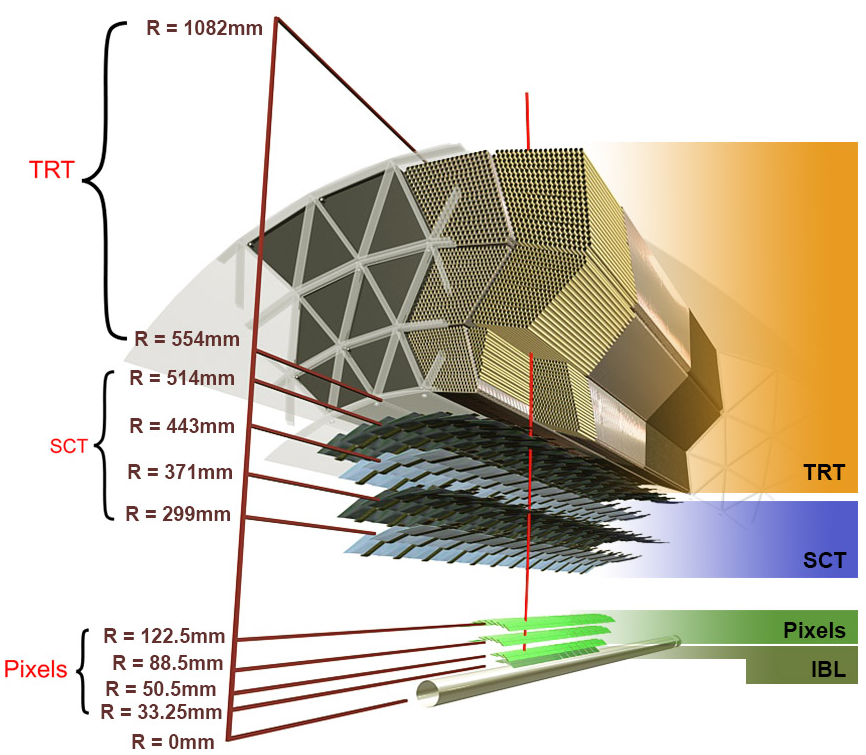
\includegraphics[width=\textwidth]{ibl}
	\end{subfigure}%
	\caption{Schematic drawing of the ID and its subdetectors. Images adapted from~\cite{Pequenao:1095926, Potamianos:2209070}.}\label{fig:ID_schematic}
\end{figure}

\subsubsection{Pixel detector}

In the high-rate environment directly adjacent to the beam pipe, the only detector technology able to operate and deliver high-precision tracking information are semiconductor detectors segmented into pixels. As opposed to strip detectors, the reduced size of silicon pixel detectors and thus significantly reduced hit rate per readout channel allows pixel detectors to still be operational in the harsh environment close to the IP. In ATLAS, pixels are hybrids of sensors and readout electronics, and were originally arranged in three layers in the barrel and the end-caps with a typical pixel of $\SI{50}{\micro\meter}\times \SI{400}{\micro\meter}$, covering pseudorapidities up to $\vert\eta\vert < 2.5$. In order to increase robustness  and performance in the high-luminosity environment, a new innermost layer, called the \gls{ibl}, was installed together with a new, smaller radius beam pipe between Run~1 and Run~2~\cite{Abbott:2018ikt,Capeans:1291633}. The IBL uses smaller pixels with a size of $\SI{50}{\micro\meter}\times \SI{250}{\micro\meter}$ and improves the tracking precision as well as vertex identification performance~\cite{Capeans:1291633}. It also improves the performance of identifying jets originating from $b$-quarks (called \textit{b}-tagging). The pixel detector~\cite{Aad:2019aic}. The tracking precision obtained by the pixel detector is $\SI{10}{\micro\meter}$ in ($R-\phi$) and $\SI{115}{\micro\meter}$ in ($z$) for the barrel and ($R$) for the end-caps.

\subsubsection{Silicon microstrip detector}

The pixel detector is surrounded by the \gls{sct}, consisting of four layers in the barrel and nine disks in the end-caps. In order to provide two-dimensional tracking information, strips are arranged in double-layers with a small crossing angle of $\SI{40}{mrad}$ and a mean pitch of $\SI{80}{\micro\meter}$~\cite{Aad:2008zzm}. A charged particle traversing the \gls{sct} through the barrel thus creates four space point measurements. In the barrel, one set of strips in each of the four double-layers is oriented in beam direction, thereby measuring $R-\phi$, and in the end-caps, one set of strips in each layer is oriented in radial direction. The \gls{sct} has roughly $6.3$ million readout channels and provides tracking information up to $\vert\eta\vert <2.5$~\cite{Aad:2008zzm}. It achieves a precision of $\SI{17}{\micro\meter}$ in ($R-\phi$) and $\SI{580}{\micro\meter}$ in ($z$) for the barrel and ($R$) for the end-caps~\cite{Aad:2008zzm}.

\subsubsection{Transition radiation tracker}

The last and also largest of the three subdetectors of the \gls{id} is the \gls{trt}, a gaseous detector made of multiple layers of $\SI{4}{\milli\meter}$ diameter drift tubes, surrounding the pixel detector and the \gls{sct}. The drift tubes consist of an aluminum cathode coated on a polyimide layer reinforced by carbon fibers and use a gold-plated tungsten wire as anode. The tubes are filled with a Xe-based gas mixture, providing an electric permittivity different from the surrounding material, causing transition radiation when traversed by ultrarelativistic particles. While the $\SI{144}{\centi\meter}$ long tubes in the barrel region are aligned parallel to the beam pipe, the $\SI{37}{\centi\meter}$ long tubes in the end-caps are aligned in radial direction, providing coverage up to $\vert\eta\vert <2.0$ and an intrinsic accuracy of $\SI{130}{\micro\meter}$ in $R-\phi$~\cite{Aad:2008zzm}. The low accuracy compared to the pixel detector and the \gls{sct} is compensated by the large amount of hits (typically $36$ per track) and the longer measured track length. As the amount of transition radiation given off by a particle, is proportional to its Lorentz factor $\gamma$~\cite{pdg2020}, the \gls{trt} is also used to improve electron identification~\cite{ATLAS-CONF-2011-128}. For the same momentum, electrons will have a higher Lorentz factor than the heavier charged pions, and consequently give off more transition radiation.

\subsection{Calorimeters}

\begin{figure}
	\centering
	\begin{subfigure}[b]{0.45\linewidth}
		\centering\includegraphics[width=\textwidth]{cal}
		\caption{Calorimeter systems\label{fig:calorimeters}}
	\end{subfigure}%
	\begin{subfigure}[b]{0.45\linewidth}
		\centering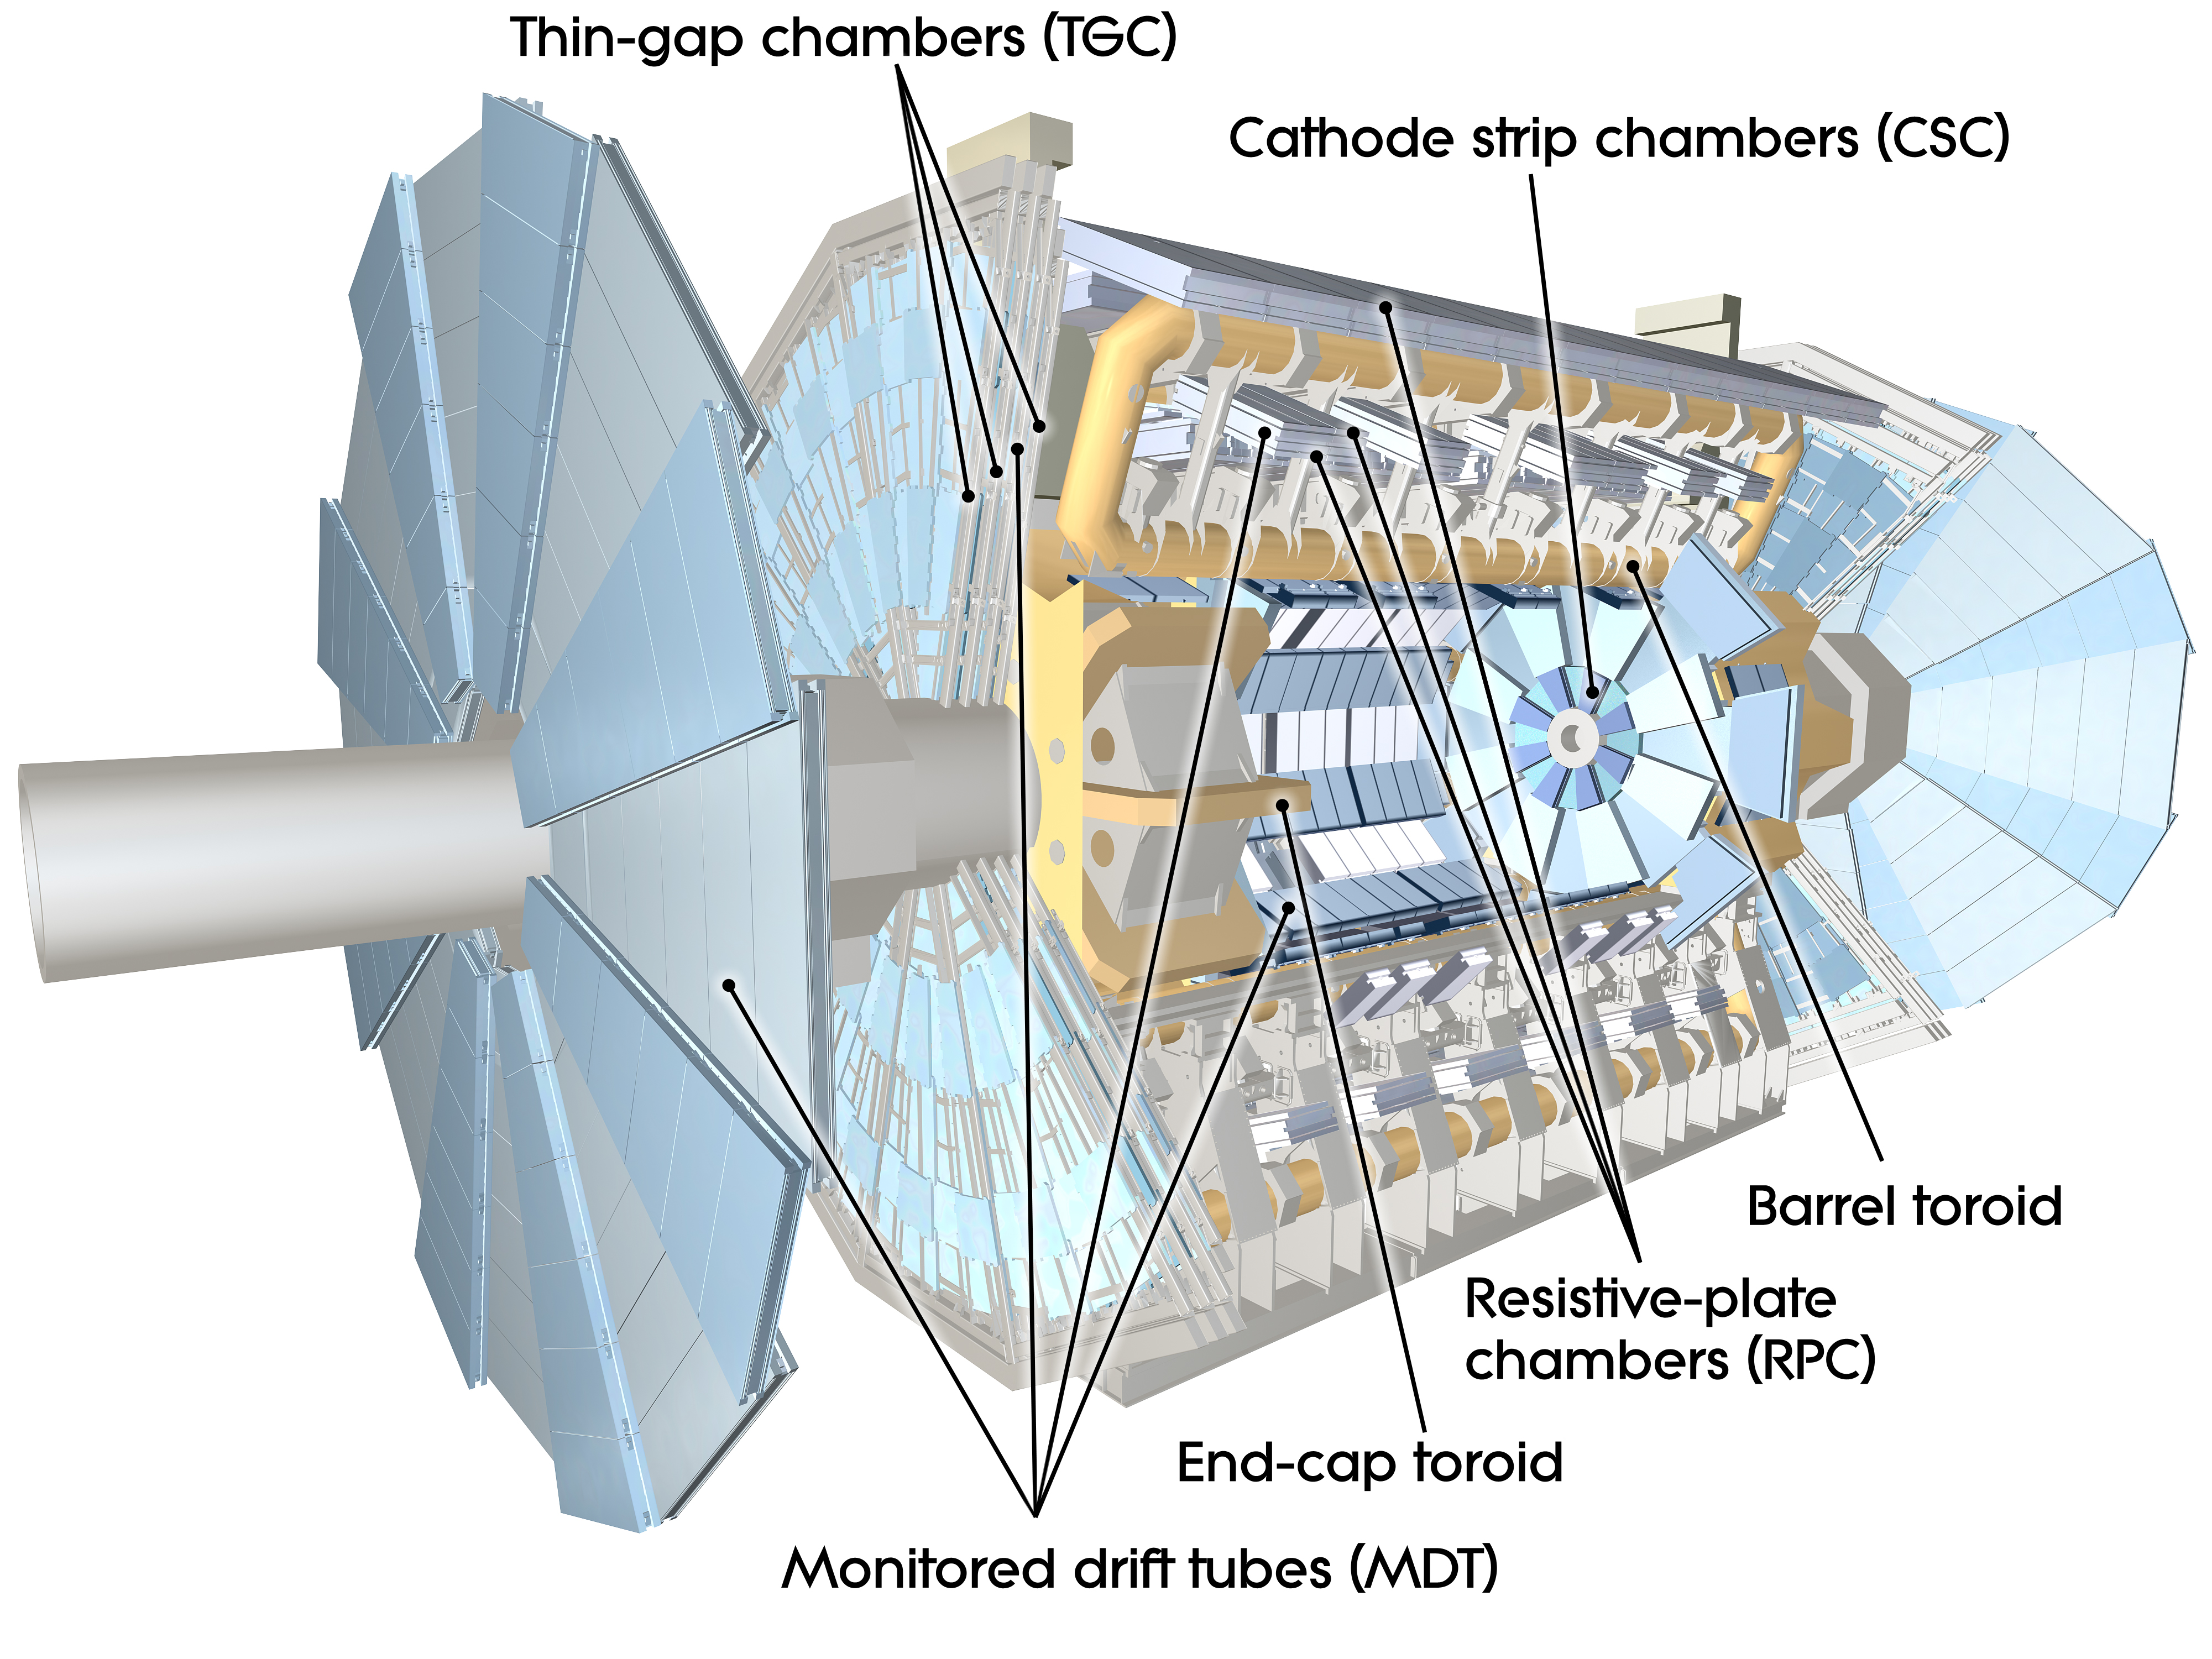
\includegraphics[width=\textwidth]{ms}
		\caption{Muon spectrometer\label{fig:muon_system}}
	\end{subfigure}%
	\caption{Schematic drawing of the calorimeter systems and the muon spectrometer in ATLAS. Images adapted from~\cite{Pequenao:1095927,Pequenao:1095929}.}\label{fig:cal_ms_schematic}
\end{figure}

The primary goal of calorimeters is to measure the energies of incoming particles by completely absorbing them. As the energies of neutral particles can not be measured by other means, calorimeters are especially important for jet energy measurements (which contain neutral hadrons)~\cite{Brock:1354959}. Since particles like photons and electrons interact mostly electromagnetically, while hadrons predominantly interact through the strong interaction, two different calorimeter types are needed in ATLAS. For values in $\eta$ matching the \gls{id}, the electromagnetic calorimeter uses a finer granularity designed for precision measurements of electrons and photons. The subsequent hadronic calorimeter uses a coarser granularity sufficient for the requirements of jet reconstruction and missing transverse moment measurements. With a coverage up to $\vert\eta\vert <4.9$, the calorimeter system in ATLAS provides the near hermetic energy measurements needed for the inference of missing transverse momentum created by neutrinos and other weakly interacting neutral particles~\cite{Aad:2008zzm}.

Both calorimeters are sampling calorimeters, consisting of alternating layers of active and absorbing material. The absorbing material interacts with the incoming particles, causing them to deposit their energy by creating cascades or \textit{showers} of secondary particles. The active layers are then used to record the shape and intensity of the produced showers. This alternating structure results in reduced material costs but also reduced energy resolution as only part of the particle's energy is sampled. Due to the typically longer cascades in hadronic interactions compared to electromagnetic interactions, and in order to minimise punch-through into the muon system, the hadronic calorimeter requires a greater material depth than the electromagnetic one. The calorimeter systems in ATLAS are schematically illustrated in \cref{fig:calorimeters}.

\subsubsection{Electromagnetic calorimeter}

The \gls{em} calorimeter has an accordion-shaped structure and uses \gls{lar} as active material and lead as absorber, providing full $\phi$ symmetry without azimuthal cracks. It is divided into a barrel part and two end-caps, covering $\vert\eta\vert <1.475$ and $1.375 < \vert\eta\vert <3.2$, respectively, and arranged in a way to provide uniform performance and resolution as a function of $\phi$. The barrel \gls{em} calorimeter consists of two identical half-barrels with a small gap of $\SI{4}{\centi\meter}$ at $z=0$. In the end-caps, the \gls{em} calorimeter consists of two coaxial wheels, covering the region $1.375 < \vert\eta\vert <2.5$ and $2.5 < \vert\eta\vert <3.2$, respectively. Calorimeter cells in the \gls{em} calorimeter are segmented into multiple layers with fine granularity in first layers in the $\eta$ region matching the ID, and coarser granularity in the outer layers and for $2.5 < \vert\eta\vert <3.2$. In order to offer good containment of electromagnetic showers, the \gls{em} calorimeter has a depth of at least $22$ ($24$) radiation lengths in the barrel (end-caps). A single instrumented \gls{lar} layer serves as presampler in the region with $\vert\eta\vert <1.8$, allowing measurements of the energy losses upstream of the \gls{em} calorimeter, \eg in the cryostats~\cite{Aad:2008zzm}. The design energy resolution of the \gls{em} calorimeter is $\sigma_E / E = 10\% / \sqrt{E} \oplus 0.7\%$~\cite{Aad:2008zzm}.

\subsubsection{Hadronic calorimeter}

Placed directly outside the envelope of the \gls{em} calorimeter is the hadronic tile calorimeter. It uses steel plates as absorber and polystyrene-based scintillating tiles as active material, and is subdivided into one central barrel and two extended barrels. Each barrel is segmented in three layers in depth with a total thickness of $7.4$ interaction lengths. The tiles are oriented radially and perpendicular to the beam pipe and grouped in 64 tile modules per barrel, resulting in a near hermetic azimuthal coverage. Wavelength shifting fibres are used to shift the ultraviolet light produced in the scintillator to visible light and guide it into photomultipliers located at the radially far end of each module. The tile calorimeter covers a region with $\vert\eta\vert <1.7$ and has a granularity of $\Delta \eta \times \Delta \phi = 0.1 \times 0.1$ except for the outermost layer which has a slightly coarser granularity in $\eta$. The design energy resolution of the tile calorimeter is $\sigma_E / E = 56.4\% / \sqrt{E} \oplus 5.5\%$~\cite{Aad:2008zzm}.

Hadronic calorimetry in the end-caps is provided by two independent calorimeter wheels per end-cap, situated directly behind the \gls{emec}. Similar to the \gls{emec}, the \gls{hec} also uses \gls{lar} calorimeter as active material, allowing both calorimeter systems to share a single cryostat per end-cap. Instead of lead, the HEC however uses copper as absorber, which not only drastically reduces the mass of a calorimeter with a given interaction length, but also improves the linearity of low-energy hadronic signals~\cite{Lee:2637852}. Each of the four wheels of the \gls{hec} is comprised of 32 wedge-shaped modules, divided into two layers in depth. The \gls{hec} provides coverage in the region with $1.5 < \vert\eta\vert <3.2$, slightly overlapping with the tile calorimeter and thus reducing the drop in material density in the transition region. While the granularity in the precision region with $1.5 < \vert\eta\vert <2.5$ is the same as for the tile calorimeter, more forward regions with large $\vert\eta\vert$ have a granularity of $\Delta \eta \times \Delta \phi = 0.2 \times 0.2$~\cite{Aad:2008zzm}. The design resolution of the \gls{hec} is $\sigma_E / E = 70.6\% / \sqrt{E} \oplus 5.8\%$~\cite{Aad:2008zzm}.


The forward region with $3.1 < \vert\eta\vert <4.9$ is covered by the \gls{lar}~\gls{fcal}, which is integrated into the end-cap cryostats. This hermetic design not only minimises energy losses in cracks between the calorimeter systems, but also reduces the amount of background reaching the muon system in the outer shell of the ATLAS experiment. In order to limit the amount of neutrons reflected into the \gls{id}, the \gls{fcal} is recessed by about $\SI{1.2}{\meter}$ with respect to the \gls{em} calorimeter, motivating a high-density design due to space constraints. The \gls{fcal} in each end-cap consists of three layers with a total depth of 10 interaction lengths. While the first layer uses copper as absorber and is optimised for electromagnetic measurements, the remaining two layers are made of tungsten and cover hadronic interactions. The metals comprising each layer are arranged in a matrix structure with electrodes consisting of rods and tubes parallel to the beam pipe filling out regular channels. The small gaps ($\SI{0.25}{\milli\meter}$ in the first layer) between the rods and tubes of the electrodes are filled with \gls{lar} as active material.

\subsection{Muon spectrometer}

Muons, being minimum ionising particles, are the only charged particles that consistently pass through the entire detector including the calorimeter system. Providing one of the cleanest signatures for \gls{bsm} physics~\cite{Brock:1354959}, muonic final states are measured with a dedicated detector system on the outermost layer of the ATLAS experiment. Embedded in the magnetic field of the toroid magnets, the \gls{ms} consists of three concentric cylindrical layers in the barrel region, and three wheels in each end-cap, and provides momentum measurements up to $\vert\eta\vert <2.7$~\cite{Aad:2008zzm}. It is designed to deliver a transverse momentum resolution of $10\%$ for $\SI{1}{\TeV}$ tracks and be able to measure muon momenta down to roughly $\SI{3}{\GeV}$.

The \gls{ms} uses two high-precision gaseous detector chamber types, \gls{mdt} chambers and \gls{csc}. As both the \gls{mdt} and \gls{csc} are drift chambers relying on charges drifting to an anode or cathode, the maximum response times of $\SI{700}{\nano\second}$ and $\SI{50}{\nano\second}$, respectively, are slow compared to the bunch-spacing of $\SI{25}{\nano\second}$. ATLAS therefore uses \gls{rpc} in the barrel and \gls{tgc} in the end-caps as triggers in order to associate measurements to the right bunch-crossing.  

\subsubsection{Monitored drift tubes}

The \gls{mdt} chambers are the main subcomponent providing precision measurements of the muon tracks up to $\vert\eta\vert <2.7$, except in the innermost end-cap layer where their coverage only extends to $\vert\eta\vert <2.0$. The \gls{mdt} are made of 3--4 layers of $\sim \SI{30}{\milli\meter}$ diameter drift tubes operated with Ar/CO$_2$ gas\footnote{With a small admixture of $\SI{300}{ppm}$ of water to improve high voltage stability.} pressurised to $\SI{3}{\bar}$. Charged particles traversing the drift tubes ionise the gas, creating electrons that drift towards a central tungsten-rhenium anode wire with a diameter of $\SI{50}{\micro\meter}$. Following the symmetry of the barrel toroid magnet, the \gls{mdt} chambers are arranged as octets around the calorimeters with the drift tubes in $\phi$ direction, \ie tangential to circles around the beam pipe. In order to be able to correct for potential chamber deformations due to varying thermal gradients, each \gls{mdt} chamber is equipped with an internal optical alignment system. Apart from the regular chambers in the barrel and the end-cap wheels, special modules are installed in order to minimise the acceptance losses due to the ATLAS support structure (the \textit{feets} of the experiment).

\subsubsection{Cathode strip chambers}

In the region with $\vert\eta\vert > 2.0$ in the first layer of the end-caps, the particle flux is too high to allow for safe operation of \gls{mdt} chambers. Instead, \gls{csc}, multiwire proportional chambers, are used for precision measurements in this region. The gold-plated tungsten-rhenium anode wires in the \gls{csc} have a diameter of $\SI{30}{\micro\meter}$ and are oriented in radial direction. The wires are enclosed on both sides by cathode planes, one segmented perpendicular to the wires (thus providing the precision coordinate), the other parallel to the wires. Each chambers is filled with an Ar/CO$_2$ gas mixture and consists of four wire planes, resulting in four measurements of $\eta$ and $\phi$ for each track. In addition to the chamber-internal alignment sensors, ATLAS also employs an optical alignment system in order to align the precision chambers to each other~\cite{Aad:2008zzm}.

\subsubsection{Resistive plate chambers}

\gls{rpc} are gaseous parallel electrode-plate chambers that use two resistive plastic laminate plates kept $\SI{2}{\milli\meter}$ apart by insulating spacers. Due to an electric field of roughly $\SI{4.9}{\kilo\volt\per\milli\meter}$ between the plates, charged particles traversing the chamber cause avalanches of charges that can be read out through capacitive coupling to metallic strips mounted on the outside of the resistive plates. In order to provide tracking information in both coordinates, each \gls{rpc} consists of two rectangular units each containing two gas volumes with a total of four pairwise orthogonal sets of readout strips. The tree concentric cylindrical layers of \gls{rpc} in the barrel region thus provide six measurements of $\eta$ and $\phi$ and cover $\vert\eta\vert <1.05$

\subsubsection{Thin gap chambers}

The \gls{tgc} are not only necessary for triggering in the end-cap \gls{ms} but also provide measurements of a second coordinate, orthogonal to the measurements of the \gls{mdt}.


\subsection{Forward detectors}

\subsection{Trigger and data acquisition system}

\subsection{Object reconstruction}


\section{Monte Carlo simulation}


%!TEX root = ../thesis.tex
%*******************************************************************************
%*********************************** Data and Monte Carlo Simulation *********
%*******************************************************************************


\chapter{Data and Monte Carlo Simulation}

\ifpdf
    \graphicspath{{chapter-mc/Figs/Raster/}{chapter-mc/Figs/PDF/}{chapter-mc/Figs/}}
\else
    \graphicspath{{chapter-mc/Figs/Vector/}{chapter-mc/Figs/}}
\fi

\section{Data}\label{sec:data}


%!TEX root = ../thesis.tex
%*******************************************************************************
%*********************************** Statistics *********
%*******************************************************************************


\chapter{Statistical data analysis}\label{ch:statistics}

\ifpdf
    \graphicspath{{chapter-statistics/Figs/Raster/}{chapter-statistics/Figs/PDF/}{chapter-statistics/Figs/}}
\else
    \graphicspath{{chapter-statistics/Figs/Vector/}{chapter-statistics/Figs/}}
\fi

In \gls{hep}, statistical models are used in order to quantify the correspondence between theoretical predictions and the experimental observations.
This chapter introduces the statistical concepts, methods and formulae used for statistical inference in this thesis.
A frequentist approach is employed, interpreting probabilities as the frequencies of the outcomes of repeatable experiments that may either be real, based on computer simulations, or mathematical abstraction~\cite{pdg2020}.
The following description largely adheres to \references\cite{Cranmer:2015nia, Cowan:2010js}.

\section{The likelihood function}\label{sec:likelihood_function}
 
In measurements in \gls{hep}, a \textit{statistical model} $f(\boldsymbol{x}\vert\boldsymbol{\phi})$ is a parametric family of \glspl{pdf} describing the probability of observing data $\boldsymbol{x}$ given a set\footnote{Sets of parameters (as opposed to single parameters) will henceforth be written using bold face.} of model parameters $\boldsymbol{\phi}$.
The latter typically describe parameters of the physical theory or unknown detector effects. The \textit{likelihood function} $L(\boldsymbol{\phi})$ is then numerically equivalent to $f(\boldsymbol{x}\vert\boldsymbol{\phi})$ with $\boldsymbol{x}$ fixed.
As opposed to the \glsfirst{pdf} $f(\boldsymbol{x})$ describing the value of $f$ as a function of $\boldsymbol{x}$ given a set of fixed parameters $\boldsymbol{\phi}$, the likelihood refers to the value of $f$ as a function of $\boldsymbol{\phi}$ given a fixed\footnote{This important difference is why the likelihood is written here as $L(\boldsymbol{\phi})$ instead of the equally common $L(\boldsymbol{x}\vert\boldsymbol{\phi})$.} value of $\boldsymbol{x}$.

Searches for \gls{bsm} physics are often\footnote{While searches for \gls{bsm} physics using unbinned distributions also exist, only binned searches are considered in the following.} centred around the measurement of several disjoint binned distributions, called \textit{channels} $c$, each associated with different event selection criteria yielding observed event counts $\boldsymbol{n}$.
In such counting experiments where each event is independently drawn from the same underlying distribution, each bin is described by a Poisson term.
The Poisson probability to observe $n$ events with an expectation of $\nu$ events, $\mathrm{Pois}(n\vert\nu)$, is given by
\begin{equation}
	\mathrm{Pois}(n\vert\nu) = \frac{\nu^n}{n!}e^{-\nu}.
\end{equation}
The expectation $\nu_{cb}$ in each channel $c$ and bin $b$ is a sum over the set of physics processes considered, called \textit{samples} in the following, 
\begin{equation}
	\nu_{cb} = \sum_{s\in\mathrm{samples}}\nu_{csb}(\boldsymbol{\eta},\boldsymbol{\chi}),
\end{equation}
where $\nu_{csb}$ is the expected sample rate in a given bin of a given channel. The sample-wise rates are in general a function of the model parameters $\boldsymbol{\phi}$ that can either be \textit{free parameters} $\boldsymbol{\eta}$ or \textit{constrained parameters} $\boldsymbol{\chi}$. Possible modifications of the expected sample rates due to model parameters are considered to be either multiplicative or additive changes to the nominal estimate $\nu_{csb}^0$ of the form
\begin{equation}
	\nu_{csb}(\boldsymbol{\eta},\boldsymbol{\chi}) = \left(\prod_i f^i_{csb}(\boldsymbol{\eta},\boldsymbol{\chi}) \right)\left(\nu^0_{csb} + \sum_j {\Delta^j_{csb}(\boldsymbol{\eta},\boldsymbol{\chi})} \right).
\end{equation}
Here, $\boldsymbol{f}(\boldsymbol{\phi})$ and $\boldsymbol{\Delta}(\boldsymbol{\phi})$ are the multiplicative and additive \textit{rate modifiers}, respectively, modifying the nominal estimates. Although in practice often only a function of a single model parameter, the rate modifiers can in general be a function of a set of model parameters.

Free parameters directly determined by the data observations are called \textit{normalisation factors}.
The constrained parameters represent the systematic uncertainties considered in the model, which---in frequentist statistics---have fixed but unknown true values.
The degree to which they cause a deviation of the expected event rates from the nominal event rates is limited through \textit{constraint terms} $c_{\boldsymbol{\chi}}(a_{\boldsymbol{\chi}}\vert\boldsymbol{\chi})$ that can be viewed as \textit{auxiliary measurements} with global observed data $\boldsymbol{a}$. 

For a given observation $\boldsymbol{x} = (\boldsymbol{n},\boldsymbol{a})$ of observed events $\boldsymbol{n}$ and auxiliary data $\boldsymbol{a}$, the likelihood then reads
\begin{equation}
	L (\boldsymbol{\eta}, \boldsymbol{\chi}) = \prod_{c\in\mathrm{channels}} \prod_{b\in\mathrm{bins_c}} \mathrm{Pois}(n_{cb}\vert\nu_{cb}(\boldsymbol{\eta},\boldsymbol{\chi})) \prod_{\chi\in\boldsymbol{\chi}}c_\chi (a_\chi\vert\chi),
\end{equation}
where, given a certain integrated luminosity, $n_{cb}$ and $\nu_{cb}$ refer to the corresponding observed and expected rate of events, respectively~\cite{ATL-PHYS-PUB-2019-029}.
Most of the systematic uncertainties are so-called \textit{interpolation parameters} $\boldsymbol{\alpha}$ representing either normalisation uncertainties or correlated shape uncertainties\improvement{Explain this further}.
Their constraint terms $c_{\boldsymbol{\alpha}}(a_{\boldsymbol{\alpha}}\vert\boldsymbol{\alpha})$ are parametrised by a Gaussian\footnote{Other parameterisations are also possible and discussed in \reference\cite{Cranmer:1456844}, but not used in the following.} with mean $a = 0$ and variance $\sigma = 1$, with $\alpha = 0$ representing the nominal value.
The \textit{up} and \textit{down} variations are then given by $\alpha=\pm 1$, thereby representing $\pm 1\sigma$ variations.
The impact of any given value of the parameter on the event rates is subsequently evaluated through polynomial interpolation and exponential extrapolation\footnote{Different interpolation and extrapolation strategies are discussed in \reference\cite{Cranmer:1456844} but not mentioned herein as they will not be used in the following.}, a method that avoids discontinuous first and second derivatives at $\alpha = 0$ and ensures positive values for the predicted event rates~\cite{Cranmer:1456844}.

Sample rates derived directly from theory calculations (\ie \gls{mc} simulation), are scaled to the integrated luminosity corresponding to the observed data.
As discussed in~\cref{sec:lumi_datataking}, the integrated luminosity is itself a measurement that is subject to uncertainties, requiring an additional constraint term in the likelihood.
It is parametrised by a Gaussian with mean corresponding to the nominal integrated luminosity measurement and standard deviation equal to the integrated luminosity measurement uncertainty.
Uncertainties arising from the finite size of the \gls{mc} datasets used to derive estimated event rates are modelled by bin-wise scale factors $\gamma_b$.
The constraint terms are Gaussian distributions with central value equal to unity and standard deviations calculated from the individual uncertainties of the samples defined in the respective channel.

As the event rate in a given bin can depend on multiple parameters, and likewise, a single parameter can affect the expected event rate in multiple bins across various channels, correlations between the model parameters $\boldsymbol{\phi}$ can occur.

The above prescription for building binned likelihoods is called the \textsc{HistFactory} template~\cite{Cranmer:1456844}. In this work, two independent implementations of the \textsc{HistFactory} template are used.
The first implementation, predominantly used in~\cref{part:simplified_model_analysis}, relies on \textsc{RooFit}~\cite{RooFit:2003ir} (using the \texttt{Minuit}~\cite{James:310399} package) and \textsc{RooStats}~\cite{RooStats:2010pm} for model parameter estimation and hypothesis tests, and is fully integrated into the \textsc{Root} data analysis framework~\cite{ROOT:1997pa,ROOT-2}. The user interface and the steering of statistical fits, as well as the bookkeeping of their results, is provided by \textsc{HistFitter}~\cite{HistFitter:2014wma}.
The second implementation, used in~\cref{part:reinterpretation}, makes use of \texttt{pyhf}~\cite{pyhf_joss,pyhf}, a recent pure-\texttt{python} implementation of \textsc{HistFactory} that is independent of the \textsc{Root} environment.
The \texttt{pyhf} implementation of \textsc{HistFactory} relies on \textsc{Numpy}~\cite{numpy} and uses computational graph libraries like \textsc{PyTorch}~\cite{pytorch}, \textsc{TensorFlow}~\cite{tensorflow2015-whitepaper} and \textsc{JAX}~\cite{jax2018github} to significantly speed up the parameter estimation process by leveraging the computational advantages of tensor algebra and automatic differentiation.
 
Apart from separating the model parameter set into free and constrained parameters $\boldsymbol{\phi} = (\boldsymbol{\eta},\boldsymbol{\chi})$, a separate partition $\boldsymbol{\phi} = (\boldsymbol{\psi},\boldsymbol{\theta})$ is frequently used in the context of hypothesis testing.
Here, $\boldsymbol{\psi}$ are so-called \textit{parameters of interests} of the model for which hypothesis tests are performed, and $\boldsymbol{\theta}$ are \textit{nuisance parameters} that are not of immediate interest but need to be accounted for to correctly model the data.
In the search presented in this work, the only \gls{poi} is the \textit{signal strength} parameter $\mu$, representing the ratio of the signal process cross section to its reference cross section as expected from theory.
The expected event rate $\nu_i$ in each bin $i$ can then be parametrised through
\begin{equation}
	\nu_b = \mu S_b + B_b,
\end{equation}
where $S_b$ and $B_b$ are the bin-wise expected signal and background rates, respectively. Fixing $\mu = 0$ thus yields an expected event rate containing only \gls{sm} processes, which is why this is also called a \textit{background-only} configuration. Setting $\mu = 1$ represents a \textit{signal-plus-background} description at nominal signal cross section. Scanning multiple values of $\mu$ allows to set limits on the visible cross sections of the signal models considered in the search. 
  
\section{Parameter estimation}

Given a likelihood $L(\boldsymbol{\phi})$ for a fixed set of observations $\boldsymbol{x}$, a measurement can be understood as a parameter estimation. In general, an estimator $\hat{\phi}$ is a function of the observed data used to estimate the true value of the model parameter $\phi$.

In particle physics, the most commonly used estimator is the \gls{mle}. The \glspl{mle} for the model parameters $\boldsymbol{\hat{\phi}}$ are defined to be the parameter values that maximise $L(\boldsymbol{\phi})$, or equivalently, maximise $\ln{L(\boldsymbol{\phi})}$ and minimise $-\ln{L(\boldsymbol{\phi})}$. The logarithm of the likelihood is used for computational reasons, as it not only reduces the computational complexity by avoiding exponentials and products, but also avoids potential problems arising from finite floating point precision. As the logarithm is a monotonically increasing function, $\ln{L(\boldsymbol{\phi})}$ has maxima at the same parameter values as ${L(\boldsymbol{\phi})}$. The negative logarithm of the likelihood is chosen in order to stick to the convention of optimisers in statistical packages typically minimising the result of a \textit{loss function}.

The \glspl{mle} $\boldsymbol{\hat{\phi}}$ can thus be found by solving the system of equations
\begin{equation}
 \frac{\partial \ln L}{\partial\phi_i} = 0,
\end{equation}
where the index $i$ runs over all parameters. Due to the complexity of the likelihood, a solution typically needs to be found numerically using minimisation algorithms. In the following, the parameter estimation is referred to as a \textit{fit} of the model to data, and the maximum likelihood estimates of the parameters are consequently called \textit{best-fit values}.

\section{Statistical tests}

In addition to estimating the values of model parameters, searches for \gls{susy} are naturally interested in claiming discovery (or alternatively exclusion) of hypothesised signal models. In the frequentist approach, this can be formulated in terms of hypothesis tests, evaluating a \textit{null hypothesis} $H_0$ against an \textit{alternative hypothesis} $H_1$, with the goal of rejecting the null hypothesis. For discovering a new signal process, $H_0$ is defined to describe only known \gls{sm} processes and thus called \textit{background-only} hypothesis. The alternative hypothesis $H_1$ is then the \textit{signal-plus-background} hypothesis describing both \gls{sm} background processes as well as the signal process considered. When excluding a signal model the signal-plus-background hypothesis takes over the role of $H_0$ and is tested against the background-only hypothesis.

The degree of agreement of observed data with a certain hypothesis $H$ is quantified by calculating a $p$-value, representing the probability of finding data of greater or more extreme incompatibility under assumption of $H$. The hypothesis can then be considered as excluded if its observed $p$-value is below a specified threshold. It is common to convert the $p$-value into a \textit{significance} $Z$, defined in such a way that a Gaussian distributed observable with measured value $Z$ standard deviations above its mean gives a one-sided upper tail probability equal to $p$. This yields the expression
\begin{equation}
	Z = \Phi^{-1}(1-p),
	\label{eq:significance}
\end{equation}
where $\Phi^{-1}$ is the quantile of the standard Gaussian. In \gls{hep}, claiming discovery of a signal conventionally requires a significance of at least $Z=5$. If the significance is lower but still $Z>3$, it is classified as a hint or evidence. For exclusion of a signal hypothesis at 95\% confidence level, a $p$-value of 0.05, \ie $Z = 1.64$, is required~\cite{Cowan:2010js}. 

The $p$-values are calculated using a \textit{test statistic} that parameterises the compatibility between the hypothesis and data in a single value. At the LHC experiments, the test statistics used for hypothesis testing are based on the \textit{profile likelihood ratio} $\lambda(\mu)$, defined to be
\begin{equation}
	\lambda(\mu) = \frac{L(\mu,\boldsymbol{\hat{\hat{\theta}}}(\mu))}{L(\hat{\mu},\hat{\boldsymbol{\theta}})},
	\label{eq:profile_likelihood}
\end{equation}
where the \glspl{cmle} $\boldsymbol{\hat{\hat{\theta}}}$ are the values of $\boldsymbol{\theta}$ that maximise the likelihood with $\mu$ fixed. The distribution of the profile likelihood ratio depends explicitly on $\mu$, and implicitly on $\boldsymbol{x} = (\boldsymbol{n},\boldsymbol{a})$, but is asymptotically  (\ie in the limit of a large number of events) independent of the nuisance parameters $\boldsymbol{\theta}$\footnote{Eliminated by choosing specific values of the nuisance parameters for a given $\boldsymbol{x}$ and $\mu$, often referred to as \textit{profiling}.} in the case where the tested value of $\mu$ is the true value $\mu'$~\cite{Cranmer:2015nia}. The asymptotic independence from $\boldsymbol{\theta}$ follows from Wilks' theorem~\cite{wilks1938} and is one of the main motivations for using the profile likelihood ratio, as it avoids the problem of having to compute $p$-values for all possible values of $\boldsymbol{\theta}$. A generalisation to tested values of $\mu$ not corresponding to the true value $\mu'$ can be derived using Wald's theorem~\cite{wald10.2307/1990256}, allowing to obtain the distribution $f(\lambda(\mu)\vert \mu',\boldsymbol{\theta})$. The profile likelihood ratio takes values between 0 and 1, with $\lambda(\mu) = 1$ corresponding to cases where the tested value of $\mu$ is in good agreement with the observed data. In \cref{eq:profile_likelihood}, the nuisance parameters result in a broadening of the profile likelihood distribution, reflecting the loss of information about $\mu$ due to systematic uncertainties~\cite{Cowan:2010js}.

As the rate of signal processes considered in the following is in general non-negative, an estimator for $\mu$ should satisfy $\hat{\mu}\geq 0$. In order to avoid the formal complications of having a boundary at $\mu = 0$, it is convenient to consider an effective estimator $\hat{\mu}$ that is allowed to become negative, provided that the respective Poisson terms for $\mu S_b + B_b$ remain positive. Imposing a constraint equivalent to requiring $\mu \geq 0$ on the test statistic itself, leads to the alternative definition of the profile likelihood as
\begin{equation}
	\tilde{\lambda}(\mu)= 
\begin{cases}
     \frac{L(\mu,\boldsymbol{\hat{\hat{\theta}}}(\mu))}{L(\hat{\mu},\hat{\boldsymbol{\theta}})}, & \hat{\mu} \geq 0,\\
     \frac{L(\mu,\boldsymbol{\hat{\hat{\theta}}}(\mu))}{L(0,\boldsymbol{\hat{\hat{\theta}}}(0))},              & \hat{\mu} < 0,
\end{cases}
\label{eq:lambda_tilde}
\end{equation}
where $\boldsymbol{\hat{\hat{\theta}}}(0)$ and $\boldsymbol{\hat{\hat{\theta}}}(\mu)$ are the \glspl{cmle} of $\boldsymbol{\theta}$ given a signal strength parameter of 0 and $\mu$, respectively. 

\subsubsection{Discovery}
For the important special case where $\mu = 0$ is tested in a model with $\mu \geq 0$, \ie discovery of a non-negative signal (rejection of the background-only hypothesis), the profile likelihood $\tilde{\lambda}(\mu)$ is used to build the test statistic
\begin{equation}
	q_0 = -2\ln{\tilde{\lambda}(0)} = 
\begin{cases}
    -2\ln{\lambda(0)}, & \hat{\mu} \geq 0,\\
    0,              & \hat{\mu} < 0.
\end{cases}
\label{eq:disc_test_stat}
\end{equation}
This definition ensures that the background-only hypothesis is not rejected due to a downward fluctuation in data, causing $\hat{\mu} < 0$. In case more events are seen in data than expected based on the background-only hypothesis, \cref{eq:disc_test_stat} produces increasingly large values of $q_0$, corresponding to an increasing incompatibility between data and the background-only hypothesis. The $p$-value quantifying the disagreement between the $\mu = 0$ hypothesis and data can then be computed using
\begin{equation}
		p_0 = \int_{q_{0,\mathrm{obs}}}^{\infty}{f(q_0\vert 0)\diff q_0},
		\label{eq:disc_pvalue}
\end{equation}
with $q_{0,\mathrm{obs}}$ the observed value of the test statistic $q_0$ in data and $f(q_0\vert 0)$ the \gls{pdf} of $q_0$ under assumption of the background-only hypothesis. In the asymptotic limit~\cite{Cowan:2010js} with a single \gls{poi}, the test statistic $q_0$ can be  written as
\begin{equation}
	q_0 = \begin{cases}
    \hat{\mu}^2/\sigma^2, & \hat{\mu} \geq 0,\\
    0,              & \hat{\mu} < 0,
\end{cases}
\label{eq:test_stat_disc_asymptotic}
\end{equation}
where $\hat{\mu}$ has a Gaussian distribution with mean $\mu '$ and variance $\sigma^2$. In the case of $\mu'=0$, the \gls{pdf} of $q_0$ has the form of a half $\chi^2$ distribution with one degree of freedom, and its cumulative distribution is $F(q_0 \vert 0) = \Phi(\sqrt{q_0})$~\cite{Cranmer:2015nia}. Using \cref{eq:significance}, the $p$-value obtained with \cref{eq:disc_pvalue} can be expressed with the significance $Z_0$ as
\begin{equation}
	Z_0 = \sqrt{q_0}.
\end{equation}


\subsubsection{Exclusion and upper limits}
If the background-only ($\mu = 0$) hypothesis cannot be rejected, the hypotheses can be switched around and instead the signal-plus-background ($\mu = 1$) hypothesis can be tested against a hypothesis where signal events are produced at a rate smaller than $\mu$. For excluding the signal-plus-background hypothesis and setting upper limits on the signal strength $\mu$, the test statistic is defined as
\begin{equation}
	\tilde{q}_\mu = 
\begin{cases}
    -2\ln{\tilde{\lambda}(\mu)}, & \hat{\mu} \leq \mu				\\
    0,              & \hat{\mu} > \mu
\end{cases} =
\begin{cases}
    -2 \ln{\frac{L(\mu,\boldsymbol{\hat{\hat{\theta}}}(\mu))}{L(\hat{\mu},\hat{\boldsymbol{\theta}})}}, & \hat{\mu} < 0,\\
    -2 \ln{\frac{L(\mu,\boldsymbol{\hat{\hat{\theta}}}(\mu))}{L(0,\boldsymbol{\hat{\hat{\theta}}}(0))}},              & 0 \leq \hat{\mu} \leq \mu, \\
    0  & \hat{\mu} > \mu.
\end{cases}
\label{eq:upper_limit_test_statistic}
\end{equation}
Setting $\tilde{q}_\mu = 0$ in the case where $\hat{\mu} > \mu$ ensures that an overfluctuation of data is not considered as evidence against the signal hypothesis. This is opposed to the definition of $q_0$, where an underfluctuation of data ($\hat{\mu} < \mu$) is not regarded to be evidence against the background-only hypothesis.
It is worth highlighting that the discovery test statistic $q_0$ in \cref{eq:disc_pvalue} is not just the special case of $\tilde{q}_\mu$ with $\mu=0$, but hinges on a different definition.
 
The $p$-value, quantifying the level of agreement between data and the tested value of $\mu$ is then given by
\begin{equation}
		p_\mu = \int_{\tilde{q}_{\mu,\mathrm{obs}}}^{\infty}{f(\tilde{q}_\mu\vert \mu)\diff \tilde{q}_\mu},
		\label{eq:pmu}
\end{equation}
where, as before, $\tilde{q}_{\mu,\mathrm{obs}}$ is the observed value of the test statistic in data and $f(\tilde{q}_\mu\vert \mu)$ is the \gls{pdf} of $\tilde{q}_\mu$ given the hypothesis $\mu$.
In the asymptotic limit~\cite{Cowan:2010js}, the test statistic $\tilde{q}_\mu$ can be written as
\begin{equation}
	\tilde{q}_\mu = 
\begin{cases}
    \mu^2/\sigma^2 - 2\mu\hat{\mu}/\sigma^2, & \hat{\mu} < 0,\\
    (\mu-\hat{\mu})^2/\sigma^2,              & 0 \leq \hat{\mu} \leq \mu, \\
    0  & \hat{\mu} > \mu,
\end{cases}
\end{equation}
which yields for the significance $Z_\mu$ the expression
\begin{equation}
	Z_\mu = 
\begin{cases}
    \sqrt{\tilde{q}_\mu}, & 0 < \tilde{q}_\mu \leq \mu^2/\sigma^2 \\
    \frac{\tilde{q}_\mu + \mu^2/\sigma^2}{2\mu/\sigma},              & \tilde{q}_\mu > \mu^2/\sigma^2 .
\end{cases}
\end{equation}

\section[CL$_s$ approach]{CL$\boldsymbol{_s}$ approach}\label{sec:cls_approach}

\begin{figure}
	\centering
	\begin{subfigure}[b]{0.45\linewidth}
		\centering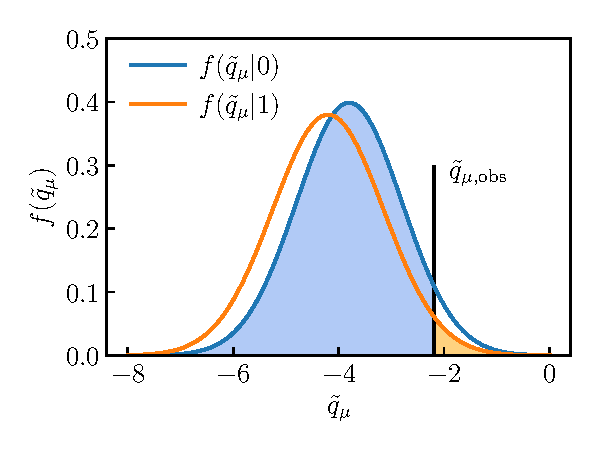
\includegraphics[width=\textwidth]{cls_1}
		\caption{\label{fig:cls_close}}
	\end{subfigure}%
	\begin{subfigure}[b]{0.45\linewidth}
		\centering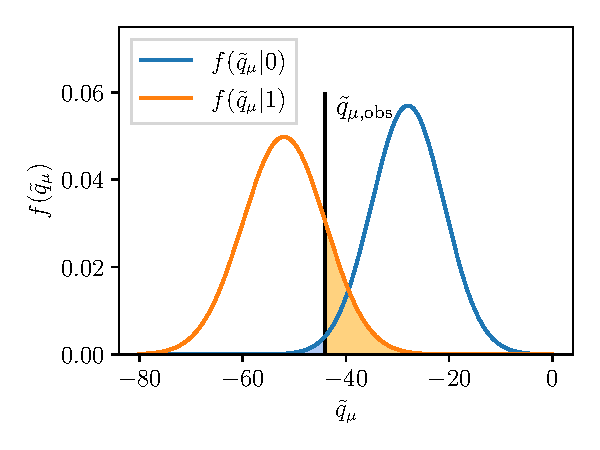
\includegraphics[width=\textwidth]{cls_2}
		\caption{\label{fig:cls_far}}
	\end{subfigure}%
	\caption{Distribution of the \glspl{pdf} of the signal plus background (in orange) and background-only (in blue) models. The orange and blue coloured areas represent the $p_{s+b}$ and $p_{b}$ values, respectively. Figure~\subref{fig:cls_close} shows a case where both \glspl{pdf} are close together, while figure \subref{fig:cls_close} shows a case where they are well separated. Figures created by the author but based on \reference\cite{Cowan:2013pha}.}\label{fig:cls_method}
\end{figure}

In the CL$_{s+b}$ method, a signal-plus-background model is excluded if $p_{s+b} < \alpha$, where $\alpha$ is defined by the desired confidence level, typically $\mathrm{CL} = 1 - \alpha = 95\%$, and $p_{s+b}$ can be calculated using the test statistic $\tilde{q}_\mu$ (with $\mu = 1$) introduced in~\cref{eq:upper_limit_test_statistic}. If the experiment has very low sensitivity to a specific signal-plus-background model, \eg because the production cross section is too low, the distribution of the test statistic of the signal-plus-background model will be very close to that of the background-only model. In case of an underfluctuation in data, the $\mu = 1$ model can then be falsely excluded, even though no sensitivity is expected. \Cref{fig:cls_method} illustrates this with a simple example. In fact, the exclusion of models to which the experiment has no sensitivity has a probability of at least $\alpha$~\cite{Cowan:2013pha}.

This problem can be remedied by adopting the CL$_s$ method~\cite{Read:2002hq}, altering the threshold for excluding a model in a way to avoid exclusion of models to which the experiment has very low sensitivity. The CL$_s$ value is defined as
\begin{equation}
	\mathrm{CL}_s = \frac{p_{s+b}}{1-p_b},
\end{equation}
where $p_b$ is the $p$-value of the background-only hypothesis\footnote{It is worth highlighting that $p_b$ is equal to $p_\mu$ from \cref{eq:pmu} with $\mu=0$. This is strictly different from $p_0$ in \cref{eq:disc_pvalue} as it relies a different test statistic.}. If the distributions of the test statistics for the signal-plus-background and the background-only models are close to each other (as seen in~\cref{fig:cls_close}) a small value of $p_{s+b}$ due to an underfluctuation in data will entail a large value of $p_b$. Consequently, in the calculation of the CL$_s$ value, $p_{s+b}$ will be penalised by $1-p_b$ (that will be close to 0), resulting in CL$_s > p_{s+b}$, preventing the exclusion of the signal-plus-background model. Conversely, in the case where the two test statistics are well-separated (see~\cref{fig:cls_far}) and $p_{s+b} < \alpha$, then $p_b$ will also be small and thus CL$_s$ will be close to $p_{s+b}$ obtained by the frequentist approach. 

\section{Asimov dataset}

Searches for \gls{bsm} physics are not only interested in the significance obtained using the dataset measured by the experiment, but also in the expected (or median) significance obtained for rejecting different values of $\mu$.
For example, for rejecting the $\mu = 1$ hypothesis, searches are interested in the expected significance obtained assuming data generated according to the $\mu = 0$ hypothesis.

The expected experimental sensitivity can be determined using an artificial dataset called the \textit{Asimov dataset}, defined such that \glspl{mle} of all parameters determined using Asimov data correspond to the true parameter values.
This is achieved by constructing a dataset where the number of events in each bin is exactly equal to the expected event rate in that bin. Using Asimov data, the Asimov likelihood $L_\mathrm{A}$ as well as the profile likelihood $\lambda_\mathrm{A}$ can be evaluated and thus a median significance can be determined.
Non-integer values for data are not an issue as factorial terms from the Poisson probabilities are canceled in the profile likelihood and can thus be dropped altogether. 

\section{Sensitivity estimation}\label{sec:sensitivity_estimation}

When designing search regions for an analysis, it is necessary to achieve an optimal signal-to-background separation power.
A significance metric is needed in order to quantify the separation power and to have a metric to optimise for.
In the following, the expected discovery significance introduced in \reference\cite{Cousins:2007bmb} is used. As the full statistical model is in general not yet known when designing the search regions, appropriate assumptions have to be made. In a \textit{cut-and-count} selection where only the total number of events after a selection are relevant (and not \eg their distribution), the significance is determined by the total number of signal events $S$, the total number of background events $B$ and the uncertainty on the expected number of background events $\Delta B$.
This can be modelled as a so-called \textit{on/off problem}\footnote{The \textit{on/off} nomenclature originates from gamma ray astronomy where \textit{on} refers to the telescope pointing on-source (measuring signal and background photons), while \textit{off} refers to it pointing off-source (measuring only background photons). This problem is an exact analog to the \gls{hep} problem herein, where the off-source measurement typically corresponds to some \textit{sideband} measurement, \ie a measurement of events in a region of a parameter disjoint from the parameter range where the signal might exist.}~\cite{Cousins:2007bmb, CRANMER_2006}, where the cut-and-count experiment uses two bins, a \gls{sr} enriched in signal events, and a \gls{cr} containing only background events.
In the background-only hypothesis, the parameter $\tau = n_\mathrm{CR} / n_\mathrm{SR}$ then denotes the ratio between the event rate in the \gls{cr}, $n_\mathrm{CR}$, and the event rate in the \gls{sr}, $n_\mathrm{SR}$.

If $\tau$ is known, then the likelihood of this simple configuration can be written in terms of the expected background event rate
\begin{equation}
	L (\mu,B) = \mathrm{Pois}(n_{\mathrm{SR}}\vert\mu S + B) \cdot \mathrm{Pois}(n_{\mathrm{CR}}\vert\tau B),
\end{equation} 
where $\mu$ is again the signal strength parameter. The relative background uncertainty can thus be treated as coming from a Poisson-distributed auxiliary measurement containing only background (\ie in the \gls{cr}) with corresponding uncertainty $\sqrt{\tau B}$, leading to the approximation
\begin{equation}
	\tau = \frac{B}{\Delta B^2}.
\end{equation}
As $n_{\mathrm{SR}}$ and $n_{\mathrm{CR}}$ are each drawn from a Poisson probability with unknown means $\nu_\mathrm{SR}$ and $\nu_\mathrm{CR}$, the background-only hypothesis corresponds exactly to the case where the ratio of Poisson means $\lambda = \nu_\mathrm{CR} / \nu_\mathrm{SR}$ is equal to $\tau$~\cite{Cousins:2007bmb}. The two Poisson terms can then be written as the product of a single Poisson term with mean $n_\mathrm{tot} = n_\mathrm{SR} + n_\mathrm{CR}$ and the binomial probability of picking $n_\mathrm{SR}$ events out of $n_\mathrm{tot}$ with probability $\rho = \nu_\mathrm{SR} / \nu_\mathrm{tot} = 1 / (1+\lambda)$. The likelihood can thus be written as
\begin{equation}
\begin{split}
	L(\mu, B) & = \mathrm{Pois} (n_\mathrm{tot}\vert\lambda_\mathrm{tot})\cdot B(n_\mathrm{SR}\vert\rho,n_\mathrm{tot}) \\ 
	& = \frac{e^{-\lambda_\mathrm{tot}}\lambda_{\mathrm{tot}}^{n_\mathrm{tot}}}{n_\mathrm{tot}\,!} \cdot{n_\mathrm{tot}\choose n_\mathrm{SR}} \rho^\lambda_\mathrm{tot} (1-\rho)^{n_\mathrm{tot}-n_\mathrm{SR}}.
\end{split}
\end{equation}

Since the background-only hypothesis cannot only be expressed as $\mu = 0$ but also as $\nu_\mathrm{SR} = \nu_B$, $\lambda = \tau$, and especially also as $\rho = 1/(1+\tau)$~\cite{Cousins:2007bmb}, its $p$-value can be calculated using the well-know frequentist binomial test,
\begin{equation}
	p_\mathrm{B} = \sum_{j=n_\mathrm{SR}}^{n_\mathrm{tot}} B (j\vert n_\mathrm{tot}, \rho).
\end{equation}
The significance corresponding to $p_\mathrm{B}$ can be derived using~\cref{eq:significance} and is computable in a numerically fast way using the incomplete beta function. The algorithm used for calculating $Z_\mathrm{B}$ in this work is implemented in the \texttt{RooStats::NumberCountingUtils} methods in \textsc{Root}~\cite{ROOT:1997pa,ROOT-2}.




%!TEX root = ../thesis.tex
%*******************************************************************************
%*********************************** Analysis Overview *********
%*******************************************************************************

\chapter{Analysis overview}\label{ch:1lepton}

\ifpdf
    \graphicspath{{chapter-analysis/Figs/Raster/}{chapter-analysis/Figs/PDF/}{chapter-analysis/Figs/}}
\else
    \graphicspath{{chapter-analysis/Figs/Vector/}{chapter-analysis/Figs/}}
\fi


This chapter aims to give an introduction to the search for electroweakinos presented in this work. First, the targeted final state, the 1-lepton final state, is introduced and motivated, followed by the \gls{sm} background processes that need to be considered when doing searches for \gls{susy} in this final state. Next the reconstruction and identification of physics objects as well as the event selection requirements are described.

\section{Search for electroweakinos in the 1-lepton final state}

In the search for electroweakinos presented herein, the simplified model introduced in \cref{sec:models_used} is interpreted in final states with one lepton, two \textit{b}-jets and high missing transverse momentum. This final state can occur when the $W$ boson decays through $W^\pm\rightarrow\ell^\pm\nu_\ell$, while the Higgs boson decays into $h\rightarrow b\bar{b}$. Although a final state without leptons would benefit from the higher branching fraction of the $W^\pm\rightarrow q'\bar{q}$ decay, due to the \gls{qcd} couplings these final states are largely dominated by \gls{qcd} multi-jet background processes that are omnipresent at hadron colliders like the \gls{lhc}. Final states with exactly one lepton have lower cross sections but allow to reject a majority of the \gls{qcd} background, as pure \gls{qcd} multi-jet events can only appear in the 1-lepton final state through false reconstruction of a jet as a lepton (so-called \textit{fake} leptons). 

Targeting the decay of the Higgs boson into a pair of \textit{b} quarks benefits from the high branching ratio of 58.3\% and allows a full reconstruction of Higgs candidates, a procedure that will be used to achieve a high signal-to-background ratio. \improvement{refer to observables} \Cref{fig:Wh_model_full} shows the full signal model targeted in this search, including the considered decays of the $W$ and Higgs bosons. 

Previous searches for electroweakinos in this final state have been performed by the ATLAS~\cite{SUSY-2013-23,SUSY-2017-01} and CMS~\cite{CMS-SUS-16-043} collaborations, excluding $\charg\neutr$ masses up to $\SI{540}{\GeV}$ and $\SI{490}{\GeV}$, respectively, for massless $\lsp$. The two previous ATLAS searches used $\SI{20.3}{\per\femto\barn}$ of $\sqrt{s}=\SI{8}{\TeV}$ and $\SI{36.1}{\per\femto\barn}$ of $\sqrt{s}=\SI{13}{\TeV}$ $pp$ collision data, respectively. As opposed to this, the search presented in the following uses the full dataset available from the Run~2 data taking period, amounting to an unprecedented $\SI{139}{\per\femto\barn}$ of $pp$ collision data at $\sqrt{s}=\SI{13}{\TeV}$.

\begin{figure}
	\centering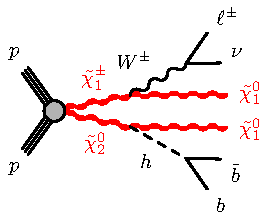
\includegraphics[width=.4\textwidth]{model_c1n2_Wh}
	\caption{Diagram for the simplified model used in this work including the decays $W^\pm\rightarrow\ell^\pm\nu_\ell$ and $h\rightarrow b\bar{b}$.}\label{fig:Wh_model_full}
\end{figure}

\section{Standard Model backgrounds}

Although the requirement of exactly one lepton isolated from surrounding hadronic activity significantly reduces the contribution from \gls{qcd} multi-jet background, numerous \gls{sm} processes can result in final states with exactly one isolated lepton, multiple jets and missing transverse momentum. Background sources are generally classified into \textit{reducible} and \textit{irreducible} backgrounds. Irreducible backgrounds are processes that have a physical phase space that is indistinguishable from the final state of the signal process considered. Reducible backgrounds, on the other hand, result from partially misreconstructed processes as well as mismeasurements. Examples of reducible processes are events where a lepton originates from a \gls{hf} decay, photon conversions or misreconstructed jets. \gls{sm} processes that result in final states with an isolated lepton, multiple jets and missing transverse momentum typically involve a $W$ boson decaying into a lepton--neutrino pair (a so-called \textit{leptonic decay}). The neutrino will contribute to the total missing transverse momentum in the event, while additional jets can appear in the final state through \gls{qcd} radiation or other branches of the decay chain.

By far the largest \gls{sm} background contributions stem from the production of top quarks, predominantly through top quark pair $\ttbar$ production, where both top quarks decay into a $W$ boson and a $b$ quark. Final states with one isolated lepton can occur through leptonic decay of one of the $W$ bosons. \Cref{fig:ttbar} shows a diagram depicting an exemplary decay of a $\ttbar$ system into a final state with one lepton, multiple jets (two of which originate from \textit{b} quarks) and missing transverse momentum. In addition to $\ttbar$, single top production (\textit{s}-channel, \texttt{t}-channel or \textit{tW}-channel) can also result in similar final states as the \gls{susy} signal and thus constitutes a significant \gls{sm} background process. An exemplary decay is shown in~\cref{fig:singletop}.

Apart from processes involving top quarks, the production of a $W$ boson in association with multiple jets ($\wjets$) is the third major background considered in the analysis. If the $W$ boson undergoes a leptonic decay and two of the produced jets are tagged as originating from $b$ quarks, the signature of this process is similar to that of signal events. An exemplary diagram for a $\wjets$ event is shown in~\cref{fig:wjets}. 

Production of multiple vector bosons $V$ ($=W,Z$)---although not a dominant background due to low cross sections---can still result in the same final state as the signal process. In the following, diboson $VV$ and multibosons $VVV$ processes are considered.

Other \gls{sm} backgrounds with small contributions in the phases spaces targeted by the analysis include $Z+\mathrm{jets}$ production, $\ttbar+V$ production, as well as various processes involving Higgs bosons. $Z+\mathrm{jets}$ plays only a minor role, as the only irreducible component is $Z(\rightarrow\tau\tau)+\mathrm{jets}$, where one $\tau$-lepton undergoes a leptonic decay and the other one a hadronic decay. Production of $\ttbar+V$ has a similar topology as ordinary $\ttbar$ processes but with lower cross section and additional objects in the final state. Higgs processes considered in the following include single Higgs production through \gls{vbf} or \gls{ggf} as well as $h+V$ and $h+\ttbar$ processes. In the following, these backgrounds are simply labelled \textit{other}. 

Pure \gls{qcd} multi-jet events can only appear in the 1-lepton final state through false reconstruction of a jet as a lepton (so-called \textit{fake} leptons) and mismeasurement of $\etmiss$. As it has been shown that this background is negligible in all selections relevant to this search, no estimation for \gls{qcd} contribution is considered in the following~\cite{SUSY-2019-08}.

\begin{figure}
	\centering
	\begin{subfigure}[b]{0.3\linewidth}
		\centering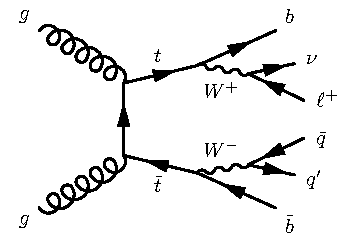
\includegraphics[width=\textwidth]{ttbar}
		\caption{\label{fig:ttbar}}
	\end{subfigure}\quad
		\begin{subfigure}[b]{0.3\linewidth}
		\centering\includegraphics[width=\textwidth]{singletop}
		\caption{\label{fig:singletop}}
	\end{subfigure}\quad
	\begin{subfigure}[b]{0.3\linewidth}
		\centering\includegraphics[width=\textwidth]{wjets}
		\caption{\label{fig:wjets}}
	\end{subfigure}
%	\begin{subfigure}[b]{0.25\linewidth}
%		\centering\includegraphics[width=\textwidth]{diboson}
%		\caption{\label{fig:diboson}}
%	\end{subfigure}
	\caption{Exemplary Feynman diagrams showing the dominant processes \subref{fig:ttbar} $t\bar{t}$, \subref{fig:singletop} single top and \subref{fig:wjets} $W+\textrm{jets}$ production with subsequent decays.}
	\label{fig:sm_backgrounds_feynman}
\end{figure}


\section{Monte Carlo samples}

\Cref{tab:mc_generators} summarises all \gls{mc} generators and software versions used for the simulated events used in the following. Further details are given in the relevant ATLAS simulation notes~\cite{ATL-PHYS-PUB-2018-009,ATL-PHYS-PUB-2016-005,ATL-PHYS-PUB-2017-006,ATL-PHYS-PUB-2017-005,ATL-PHYS-PUB-2016-002}.

\subsection{Signal samples}

The $\charg\neutr$ pair production signal samples were generated at \gls{lo} using \textsc{MadGraph5\_aMC@NLO} 2.6.2~\cite{MGaMCNLO:2014hca,Frederix:2012ps} with up to two additional partons in the \gls{me}. \textsc{MadGraph5\_aMC@NLO} is interfaced with \textsc{Pythia8}~\cite{Pythia8:2007gs} for the \gls{ps}, hadronisation and underlying event, using the CKKW-L~\cite{Lonnblad:2011xx} scheme for matching the \gls{ps} to the \glspl{me}. The NNPDF 2.3 LO~\cite{Ball:2012cx} \gls{PDF} set and the A14 set of tuned parameters~\cite{ATL-PHYS-PUB-2014-021} are used. For modelling the decay of \gls{hf} quarks, \textsc{EvtGen}~\cite{Lange:2001uf} v1.6 is used. 

As the $\charg/\neutr$ and $\lsp$ masses are free parameters of the signal model, they are systematically scanned, resulting in a set of 164 distinct evenly distributed in the two-dimensional grid spanned by the mass parameters. In the following the two-dimensional grid will be referred to as \textit{signal grid}, while the distinct signal scenarios (each witch a unique set of mass parameter values) will be referred to as \textit{signal point}. The generated signal grid covers $\charg/\neutr$ masses from $\SI{150}{\GeV}$ to $\SI{1.1}{\TeV}$ and $\lsp$ masses from $\SI{0}{\GeV}$ to $\SI{550}{\GeV}$, avoiding the kinematically forbidden region with $m(\charg/\neutr) < m(\lsp) + m(h)$.

Signal samples well within the expected sensitivity range of the analysis (with relatively low $\charg/\neutr$ and $\lsp$ masses) are generated using the \textsc{ATLFAST-II} detector simulation, while the full detector simulation using \textsc{Geant4} is used for the remaining model points for maximum accuracy. In order to account for pileup effects, all signal samples are overlaid with simulated minimum bias events generated using \textsc{Pythia8} and the A3 tune~\cite{ATL-PHYS-PUB-2016-017}, reweighted to match the pileup distribution measured in data. 

The cross sections for chargino pair production have been calculated using \textsc{Resummino}~\cite{Fuks:2013vua} at \gls{nlo} in the strong coupling constant and including \gls{nll} terms in the soft gluon resummation~\cite{Fiaschi:2018hgm,Fuks:2012qx}.

\subsection{Background samples}

Top pair production and single top processes were generated using \textsc{Powheg-Box} v2~\cite{PowhegBox:2010xd}, implementing the \textsc{POWHEG} method~\cite{Powheg1,Powheg2} for merging \gls{nlo} \glspl{me} with the \glspl{ps}. The \gls{ps}, hadronisation and underlying event were simulated using \textsc{Pythia8} with the A14 tune. Production of $\ttbar$ in association with a vector boson $\ttbar+V$ are generated using \textsc{MadGraph5\_aMC@NLO} 2.3.3, interfaced with \textsc{Pythia8} for the \gls{ps}. The set of \glspl{PDF} used for simulation of $\ttbar$, single top, and $\ttbar+V$ is the NNPDF2.3LO set.

Production of a vector boson $V$ with additional jets ($V+\mathrm{jets}$) is simulated using \textsc{Sherpa} 2.2.1~\cite{Gleisberg:2008ta,Bothmann:2019yzt}, allowing up to two (four) additional parton emissions at NLO (LO) accuracy. The CKKW \gls{me}+\gls{ps} matching and merging scheme~\cite{Hoeche:2009rj,Catani:2001cc}, extended to NLO accuracy~\cite{Hoeche:2012yf}. Diboson ($VV$) and multiboson ($VV$) is simulated using \textsc{Sherpa} 2.2.1 and 2.2.2. The \glspl{PDF} used are provided by the NNPDF3.0NNLO set~\cite{Ball:2014uwa} and the generator tune is the default \textsc{Sherpa} tune.

All Higgs processes are simulated using \textsc{Powheg-Box} v2 for the \gls{me} calculations and \textsc{Pythia8} for the \gls{ps}, underlying event and hadronisation. While the generation of $h+\ttbar$ uses the A14 tune and the NNPDF2.3LO set, $h+V$ and single Higgs production are simulated using the NNPDF 3.0 NNLO set and the AZNLO~\cite{ATL-PHYS-PUB-2013-017} set of tuned generator parameters.

The detector simulation for all \gls{mc} background samples was performed using the full detector simulation based on \textsc{Geant4}, introduced in \cref{sec:detector_simulation}. Except for the \gls{mc} samples generated using \textsc{Sherpa}, all background samples use \textsc{EvtGen} v1.2 or v1.6 to model the decay of \gls{hf} quarks. Similar to the signal models, all background samples are mixed with simulated minimum bias events generated with \textsc{Pythia8} and the A3 tune.

\begin{table}
	\centering
	\setlength\heavyrulewidth{0.2ex}
	\small
	\caption{Overview of configuration of \gls{mc} generators used for simulating the various signal and \gls{sm} background processes.}
	\resizebox{\textwidth}{!}{\begin{tabular} {llllll}
	\toprule
	Process & Matrix element & Parton shower & PDF set & Cross section & Tune\\ 
	\midrule
	Signal & \textsc{MadGraph5\_aMC@NLO} 2.6.2 & \textsc{Pythia} 8.230 & NNPDF 2.3 LO & NLO+NLL~\cite{Fuks:2013vua,Fiaschi:2018hgm,Fuks:2012qx} & A14 \\
	\midrule	
	$\ttbar$ & \textsc{Powheg-Box} & \textsc{Pythia} 8.230 & NNPDF2.3LO & NNLO+NNLL~\cite{Czakon:2011xx,Cacciari:2011hy} & A14 \\
	$t$ (s-channel) & \textsc{Powheg-Box} & \textsc{Pythia} 8.230 & NNPDF2.3LO & NLO~\cite{Kant:2014oha} & A14 \\
	$t$ (t-channel) & \textsc{Powheg-Box} & \textsc{Pythia} 8.230 & NNPDF2.3LO & NLO~\cite{Kant:2014oha} & A14 \\
	$t+W$ & \textsc{Powheg-Box} & \textsc{Pythia} 8.230 & NNPDF2.3LO & NNLO~\cite{Kant:2014oha,Kidonakis:2010ux,} & A14 \\
	$\ttbar + V$ & \textsc{MadGraph5\_aMC@NLO} 2.3.3 & \textsc{Pythia} 8.210 & NNPDF2.3LO & NLO~\cite{Campbell:2012dh,Lazopoulos:2008de} & A14 \\
	\midrule
	$V+\mathrm{jets}$ & \multicolumn{2}{c}{\textsc{Sherpa} 2.2.1} & NNPDF3.0NNLO & NNLO~\cite{Gavin:2010az} & \textsc{Sherpa} default \\
	$VV$ & \multicolumn{2}{c}{\textsc{Sherpa} 2.2.1/2.2.2} & NNPDF3.0NNLO & NLO~\cite{ATL-PHYS-PUB-2017-005} & \textsc{Sherpa} default\\
	$VVV$ & \multicolumn{2}{c}{\textsc{Sherpa} 2.2.1/2.2.2} & NNPDF3.0NNLO & NLO~\cite{ATL-PHYS-PUB-2017-005} & \textsc{Sherpa} default\\
	\midrule
	$h+\ttbar$ & \textsc{Powheg-Box} & \textsc{Pythia} 8.230 & NNPDF2.3LO & NLO~\cite{deFlorian:2016spz} & A14 \\
	$h+V$ & \textsc{Powheg-Box} & \textsc{Pythia} 8.212 & NNPDF3.0NNLO & NNLO~\cite{deFlorian:2016spz} & AZNLO \\
	\textit{h (ggF)} & \textsc{Powheg-Box} & \textsc{Pythia} 8.212 & NNPDF3.0NNLO & N$^3$LO+N$^3$LL~\cite{deFlorian:2016spz} & AZNLO \\
	\textit{h (VBF)} & \textsc{Powheg-Box} & \textsc{Pythia} 8.212 & NNPDF3.0NNLO & NNLO~\cite{deFlorian:2016spz} & AZNLO \\
	\bottomrule
	\end{tabular}}\vspace{3mm}
	\label{tab:mc_generators}   
\end{table}

\section{Object definitions}

\subsection{Electrons}

\subsection{Muons}

\subsection{Jets}

\subsection{\textit{b}-tagging}

\subsection{Missing transverse momentum}

\section{Overlap removal}

\section{Event selection}

\section{Triggers}
%!TEX root = ../thesis.tex
%*******************************************************************************
%*********************************** Conclusions *********
%*******************************************************************************

%\titleformat{\chapter}[display]
%	{\normalfont\LARGE}
%	{\filleft\MakeUppercase{\chaptertitlename}\hspace{0.5cm}\rlap{\resizebox{!}{1.5cm}{\thechapter}~\rule{5cm}{1.5cm}}\hspace{0.5cm}}
%  	{10pt}
%  	{\bf\LARGE\filright}
%\titlespacing*{\chapter}{0pt}{30pt}{20pt}

\chapter{Conclusions}

\ifpdf
    \graphicspath{{chapter-summary/Figs/Raster/}{chapter-summary/Figs/PDF/}{chapter-summary/Figs/}}
\else
    \graphicspath{{chapter-summary/Figs/Vector/}{chapter-summary/Figs/}}
\fi


This thesis presented a search for direct production of electroweakinos in events with one lepton, missing transverse momentum and a Higgs boson decaying into two \textit{b}-jets.
The full dataset of Run~2 of the \gls{lhc}, amounting to \onethirtynineifb of $pp$ collisions at $\sqrt{s} = \SI{13}{\TeV}$, recorded with the ATLAS experiment, was analysed.
The search targets a simplified electroweakino ($\charg\neutr$) pair-production model with subsequent decays into $W$ and Higgs bosons together with two lightest neutralinos ($\lsp$). The $\lsp$ is the \gls{lsp} of the model, is electrically neutral and stable, and thus could be a good candidate for \gls{dm}.
It escapes the detector without leaving a trace, resulting, in general, in a significant amount of missing transverse momentum that can be triggered on.
The search further targets a $W$ boson decay into a lepton--neutrino pair and a Higgs boson decay into a \textit{b}-jet pair.

Both the lepton--neutrino and the \textit{b}-jet pairs offer powerful discriminative handles, exploited through the use of a number of kinematic observables in order to maximise the signal-to-background ratio in the phase space targeted.
Using a dedicated optimisation procedure, two sets of signal regions are defined, one targeting generic \gls{bsm} scenarios (called \textit{discovery} signal regions), and one optimised for the simplified model in question (called \textit{exclusion} signal regions). 
The exclusion signal regions are designed to be mutually exclusive through their requirements on the transverse mass ($\mt$) and the contransverse mass ($\mct$).
Contributions from \gls{sm} background processes in the signal regions originate primarily from $\ttbar$ and single top production, as well as $\wjets$ processes. Contributions from \gls{sm} backgrounds are estimated either with a semi-data-driven technique using dedicated control regions, or directly from \gls{mc} simulation.
A binned likelihood is constructed, statistically combining all exclusion signal regions into a two-dimensional shape-fit that exploits the varying shapes of the $\mt$ and $\mct$ distributions of \gls{susy} signal and \gls{sm} background processes. This approach allows to achieve sensitivity to a wide variety of kinematic regimes.
%A combined likelihood containing terms for all control and signal regions including all systematic uncertainties considered was constructed and fit to data. 

No significant excess has been observed in any of the signal regions, and thus model-dependent exclusion limits and model-independent upper limits on the visible cross section of \gls{bsm} processes have been derived.
Due to the introduction of the two-dimensional shape-fit and the unprecedented amount of \onethirtynineifb of \textit{pp} collision data analysed, the model-dependent exclusion limits set by previous searches targeting the same simplified model can be significantly extended.
For a massless \gls{lsp}, $\charg/\neutr$ masses up to $\SI{740}{\GeV}$ can be excluded at 95\% CL. In the case of a heavier \gls{lsp} with $m(\lsp)\approx\SI{250}{\GeV}$, the limits on the $\charg/\neutr$ masses weaken to about $\SI{600}{\GeV}$.
At the time of writing, the limits obtained by this search represent the most stringent constraints on $\charg\neutr$ pair-production set by ATLAS in the context of the simplified model considered~\cite{ATL-PHYS-PUB-2020-020}.
The model-independent 95\% CL upper limits on the visible cross section of \gls{bsm} processes vary between $\SI{0.26}{\femto\barn}$ and $\SI{0.11}{\femto\barn}$, depending on the signal region considered. 

The absence of physics beyond the \gls{sm} in the Run~2 dataset of the \gls{lhc} in the search presented herein, is in line with the results of other \gls{susy} searches performed by ATLAS and CMS.
While the existence of gluinos and squarks at the $\SI{}{\TeV}$-scale was already severely challenged by the end of Run~1 of the \gls{lhc}, the limits on electroweakinos and sleptons were, in general, weaker because of their smaller production cross sections.
Due to the large integrated luminosity available through the Run~2 dataset, and the improved analysis techniques and strategies developed over the last years, the limits on electroweakinos and sleptons are also significantly increasing, and in some cases start to approach the $\SI{1}{\TeV}$ mark~\cite{ATL-PHYS-PUB-2020-020,SUSY-2018-32}. 
%The diverse \gls{susy} search programs at ATLAS and CMS thus heavily constrain the existence of \gls{susy} at the $\SI{}{\TeV}$ scale.

Given these constraints, it might be tempting to discard the existence of \gls{susy} at the \gls{lhc} altogether. Such conclusions would, however, be drawn much too early.
On the one hand, \onethirtynineifb of \textit{pp} collision data only corresponds to a fraction of the total integrated luminosity the \gls{lhc} is designed to deliver. By the end of the lifetime of the high-luminosity \gls{lhc} upgrade, a projected amount of $\SI{3000}{\per\femto\barn}$~\cite{Apollinari:2116337} will have been delivered to the particle physics experiments.
Many supersymmetric models not accessible with the Run~2 dataset using today's analyses, will hence only come into reach in the upcoming runs of the \gls{lhc}.
On the other hand, most limits derived by \gls{susy} searches assume specific simplified models and are thus only valid in the context of the assumptions made in these models.
In any realistic \gls{susy} scenario, assumptions like 100\% branching ratios or small sets of participating, non-decoupled supersymmetric particles are, however, most likely not exactly fulfilled.
Thus, simplified model limits can in general not be trivially interpreted as the true underlying constraints on the respective parameters of a realistic \gls{susy} scenario.
 
Due to the rapidly changing landscape of models for physics beyond the \gls{sm} and the limited scope of parameter limits quoted by the experiments, reinterpretations of searches for supersymmetry are highly desirable and see significant interest from both the experimental and theory communities.
With this in mind, the search for \gls{susy} presented herein was implemented to be fully reinterpretable in the light of new \gls{bsm} models.
This is achieved by using a cyber-infrastructure called \textsc{Recast}~\cite{RECAST_cranmer}, relying on containerised workflows orchestrating parametrised job templates.
Additionally, the full likelihood of the search was made publicly available in a readily available format, allowing it to be incorporated in a number of reinterpretation efforts outside of ATLAS~\cite{SModelS_pyhf:2020grj,Goodsell:2020ddr}. 
 
Large-scale reinterpretations in high-dimensional model spaces are especially interesting, but computationally extremely challenging, and thus require suitable approximations. In this thesis, a method to generically approximate the likelihoods of \gls{susy} searches using binned distributions was introduced and validated using a selection of ATLAS searches for \gls{susy}.
The search previously presented was reinterpreted in the \gls{pmssm}, a 19-dimensional parameter space containing more realistic \gls{susy} scenarios (compared to simplified models). Due to the assumption of 100\% branching fractions not being satisfied in many of these more complete \gls{susy} scenarios, the sensitivity of the \onelepton search was found to be noticeably reduced. A small fraction of models sampled could, however, still be excluded.

The impact of the \onelepton search on electroweakino masses was investigated, revealing some sensitivity to $\tilde{\chi}_2^\pm\neutr$ production with a wino-like \gls{lsp}, in addition to sensitivity towards models phenomenologically close to the simplified model the search was optimised for.
The impact of the \onelepton search on the \gls{dm} relic density was also investigated.
While no conclusive statement could be made for models with a bino-like $\lsp$ because of the limited number of such models sampled in the relevant parameter space, some models with a wino-like $\lsp$ with cosmological abundance satisfying the Planck constraint could still be excluded. 
 
 Although hopes of quickly finding supersymmetric particles with the \gls{lhc} have not materialised, there is still a possibility of finding hints for physics beyond the \gls{sm} in the collision data recorded by the \gls{lhc} experiments.
 Considerable regions of the parameter space of realistic \gls{susy} scenarios are still largely unconstrained and offer ample space for \gls{susy} to hide in.
 In order to provide a comprehensive overview of the constrained parameter space, it is not only important to optimise searches to be sensitive to the complex phenomenology of realistic supersymmetric scenarios, but also to design the searches to be systematically reinterpretable, especially in light of more complete and realistic scenarios.
 After all, searches for \gls{bsm} physics are the tools that shine a light on the otherwise unilluminated landscapes of the parameter spaces of \gls{bsm} theories.
 Allowing these tools to be reusable significantly increases the area of parameter space they can shine a light onto.    
 

% ********************************** Back Matter *******************************
% Backmatter should be commented out, if you are using appendices after References


% ********************************** Appendices ********************************

%\begin{appendices} % Using appendices environment for more functionality
%	
%	%!TEX root = ../thesis.tex
% ******************************* Thesis Appendix A ****************************

\chapter{}
\section{Additional information on signal region optimisation}\label{app:n-1_plots_cut_opt}

\ifpdf
\graphicspath{{chapter-optimisation/Figs/Raster/}{chapter-electroweak/Figs/PDF/}{chapter-optimisation/Figs/}}
\else
\graphicspath{{chapter-optimisation/Figs/Vector/}{chapter-electroweak/Figs/}}
\fi

The following figures provide additional information on the signal region optimisation performed in~\cref{ch:signal_region_optimisation}. \Cref{fig:results_z_vs_eff_rest} shows the results of the $N$-dimensional cut scan for the remaining benchmark signal points considered. As before, three different uncertainty configurations are used for computing the significance $Z_\mathrm{B}$, and all values are computed for the two statistically independent subsets used during the $N$-dimensional scan. This approach allows to gauge the impact of statistical fluctuations on the cut combinations tested.

By choosing a well-performing cut combination for each benchmark point, the optimised selections in~\cref{fig:results_n1_800_0,fig:results_n1_800_150,fig:results_n1_800_250,fig:results_n1_600_300,fig:results_n1_400_200,fig:results_n1_300_150} are found after a round of $N-1$ plots. As discussed in~\cref{sec:towards_signal_regions} the optimal cut combinations for each benchmark signal point are consolidated in different signal regions designed to be sensitive to different kinematic regions of the model parameter space. 

\Cref{fig:results_HF_scan_app} shows additional information on some of the investigated shape-fit configurations. Two-dimensional shape-fits in $(\mt,\mbb)$, $(\mt,\met)$ and $(\mt,\mct)$ are compared, showing 

\begin{figure}[hb]
	\centering
	\begin{subfigure}[b]{0.5\linewidth}
		\centering\includegraphics[width=1.0\textwidth]{N-1_cut_scan/z_vs_effs_800_150.pdf}
		\caption{$m(\charg/\neutr), m(\lsp) =  800, \SI{150}{\GeV}$}
	\end{subfigure}\hfill
	\begin{subfigure}[b]{0.5\linewidth}
		\centering\includegraphics[width=1.0\textwidth]{N-1_cut_scan/z_vs_effs_800_0.pdf}
		\caption{$m(\charg/\neutr), m(\lsp) =  800, \SI{0}{\GeV}$}
	\end{subfigure}\hfill
	\begin{subfigure}[b]{0.5\linewidth}
		\centering\includegraphics[width=1.0\textwidth]{N-1_cut_scan/z_vs_effs_600_300.pdf}
		\caption{$m(\charg/\neutr), m(\lsp) =  600, \SI{300}{\GeV}$}
	\end{subfigure}\hfill
	\begin{subfigure}[b]{0.5\linewidth}
		\centering\includegraphics[width=1.0\textwidth]{N-1_cut_scan/z_vs_effs_400_200.pdf}
		\caption{$m(\charg/\neutr), m(\lsp) =  400, \SI{200}{\GeV}$}
	\end{subfigure}\hfill

	\caption[N-dimensional cut scan results]{Results of the $N$-dimensional cut scan for the remaining four benchmark points. The binomial discovery significance $Z_\mathrm{B}$ is plotted against the signal efficiency for varying uncertainty configurations. Additionally, the expected \gls{sm} background rates are shown, including statistical uncertainty for one of the two statistically independent samples (shaded area). The solid and dashed lines represent the two statistically independent subset that the \gls{mc} samples are split into.}
	\label{fig:results_z_vs_eff_rest}
\end{figure}


\begin{figure}
	\centering
	\begin{subfigure}[b]{0.5\linewidth}
		\centering\includegraphics[width=0.9\textwidth]{N-1_cut_scan/n1_800_0/mt}
	\end{subfigure}\hfill
	\begin{subfigure}[b]{0.5\linewidth}
		\centering\includegraphics[width=0.9\textwidth]{N-1_cut_scan/n1_800_0/mct}
	\end{subfigure}\hfill
	\begin{subfigure}[b]{0.5\linewidth}
		\centering\includegraphics[width=0.9\textwidth]{N-1_cut_scan/n1_800_0/met}
	\end{subfigure}\hfill
	\begin{subfigure}[b]{0.5\linewidth}
		\centering\includegraphics[width=0.9\textwidth]{N-1_cut_scan/n1_800_0/mlb1}
	\end{subfigure}\hfill
	\begin{subfigure}[b]{0.5\linewidth}
		\centering\includegraphics[width=0.9\textwidth]{N-1_cut_scan/n1_800_0/mbb_both}
	\end{subfigure}\hfill
	\begin{subfigure}[b]{0.5\linewidth}
		\centering\includegraphics[width=0.9\textwidth]{N-1_cut_scan/n1_800_0/nJet30}
	\end{subfigure}

	\caption[N-1 plots for the chosen cut combination for the (800, 0) signal point]{N-1 plots for the chosen cut combination for the $(m(\charg/\neutr), m(\lsp)) = (\SI{800}{\GeV}, \SI{0}{\GeV})$ signal point. The shaded region includes \gls{mc} statistical uncertainty as well as 30\% systematic uncertainty (added in quadrature) on the background. The significance is computed using the binomial discovery significance using the uncertainty on the background.}
	\label{fig:results_n1_800_0}
\end{figure}



\begin{figure}
	\centering
	\begin{subfigure}[b]{0.5\linewidth}
		\centering\includegraphics[width=0.9\textwidth]{N-1_cut_scan/n1_800_150/mt}
	\end{subfigure}\hfill
	\begin{subfigure}[b]{0.5\linewidth}
		\centering\includegraphics[width=0.9\textwidth]{N-1_cut_scan/n1_800_150/mct}
	\end{subfigure}\hfill
	\begin{subfigure}[b]{0.5\linewidth}
		\centering\includegraphics[width=0.9\textwidth]{N-1_cut_scan/n1_800_150/met}
	\end{subfigure}\hfill
	\begin{subfigure}[b]{0.5\linewidth}
		\centering\includegraphics[width=0.9\textwidth]{N-1_cut_scan/n1_800_150/mlb1}
	\end{subfigure}\hfill
	\begin{subfigure}[b]{0.5\linewidth}
		\centering\includegraphics[width=0.9\textwidth]{N-1_cut_scan/n1_800_150/mbb_both}
	\end{subfigure}\hfill
	\begin{subfigure}[b]{0.5\linewidth}
		\centering\includegraphics[width=0.9\textwidth]{N-1_cut_scan/n1_800_150/nJet30}
	\end{subfigure}

	\caption[N-1 plots for the chosen cut combination for the (800, 150) signal point]{N-1 plots for the chosen cut combination for the $(m(\charg/\neutr), m(\lsp)) = (\SI{800}{\GeV}, \SI{150}{\GeV})$ signal point. The shaded region includes \gls{mc} statistical uncertainty as well as 30\% systematic uncertainty (added in quadrature) on the background. The significance is computed using the binomial discovery significance using the uncertainty on the background.}
	\label{fig:results_n1_800_150}
\end{figure}

\begin{figure}
	\centering
	\begin{subfigure}[b]{0.5\linewidth}
		\centering\includegraphics[width=0.9\textwidth]{N-1_cut_scan/n1_800_250/mt}
	\end{subfigure}\hfill
	\begin{subfigure}[b]{0.5\linewidth}
		\centering\includegraphics[width=0.9\textwidth]{N-1_cut_scan/n1_800_250/mct}
	\end{subfigure}\hfill
	\begin{subfigure}[b]{0.5\linewidth}
		\centering\includegraphics[width=0.9\textwidth]{N-1_cut_scan/n1_800_250/met}
	\end{subfigure}\hfill
	\begin{subfigure}[b]{0.5\linewidth}
		\centering\includegraphics[width=0.9\textwidth]{N-1_cut_scan/n1_800_250/mlb1}
	\end{subfigure}\hfill
	\begin{subfigure}[b]{0.5\linewidth}
		\centering\includegraphics[width=0.9\textwidth]{N-1_cut_scan/n1_800_250/mbb_both}
	\end{subfigure}\hfill
	\begin{subfigure}[b]{0.5\linewidth}
		\centering\includegraphics[width=0.9\textwidth]{N-1_cut_scan/n1_800_250/nJet30}
	\end{subfigure}

	\caption[N-1 plots for the chosen cut combination for the (800, 250) signal point]{N-1 plots for the chosen cut combination for the $(m(\charg/\neutr), m(\lsp)) = (\SI{800}{\GeV}, \SI{250}{\GeV})$ signal point. The shaded region includes \gls{mc} statistical uncertainty as well as 30\% systematic uncertainty (added in quadrature) on the background. The significance is computed using the binomial discovery significance using the uncertainty on the background.}
	\label{fig:results_n1_800_250}
\end{figure}

\begin{figure}
	\centering
	\begin{subfigure}[b]{0.5\linewidth}
		\centering\includegraphics[width=0.9\textwidth]{N-1_cut_scan/n1_600_300/mt}
	\end{subfigure}\hfill
	\begin{subfigure}[b]{0.5\linewidth}
		\centering\includegraphics[width=0.9\textwidth]{N-1_cut_scan/n1_600_300/mct}
	\end{subfigure}\hfill
	\begin{subfigure}[b]{0.5\linewidth}
		\centering\includegraphics[width=0.9\textwidth]{N-1_cut_scan/n1_600_300/met}
	\end{subfigure}\hfill
	\begin{subfigure}[b]{0.5\linewidth}
		\centering\includegraphics[width=0.9\textwidth]{N-1_cut_scan/n1_600_300/mlb1}
	\end{subfigure}\hfill
	\begin{subfigure}[b]{0.5\linewidth}
		\centering\includegraphics[width=0.9\textwidth]{N-1_cut_scan/n1_600_300/mbb_both}
	\end{subfigure}\hfill
	\begin{subfigure}[b]{0.5\linewidth}
		\centering\includegraphics[width=0.9\textwidth]{N-1_cut_scan/n1_600_300/nJet30}
	\end{subfigure}

	\caption[N-1 plots for the chosen cut combination for the (600, 300) signal point]{N-1 plots for the chosen cut combination for the $(m(\charg/\neutr), m(\lsp)) = (\SI{600}{\GeV}, \SI{300}{\GeV})$ signal point. The shaded region includes \gls{mc} statistical uncertainty as well as 30\% systematic uncertainty (added in quadrature) on the background. The significance is computed using the binomial discovery significance using the uncertainty on the background.}
	\label{fig:results_n1_600_300}
\end{figure}

\begin{figure}
	\centering
	\begin{subfigure}[b]{0.5\linewidth}
		\centering\includegraphics[width=0.9\textwidth]{N-1_cut_scan/n1_400_200/mt}
	\end{subfigure}\hfill
	\begin{subfigure}[b]{0.5\linewidth}
		\centering\includegraphics[width=0.9\textwidth]{N-1_cut_scan/n1_400_200/mct}
	\end{subfigure}\hfill
	\begin{subfigure}[b]{0.5\linewidth}
		\centering\includegraphics[width=0.9\textwidth]{N-1_cut_scan/n1_400_200/met}
	\end{subfigure}\hfill
	\begin{subfigure}[b]{0.5\linewidth}
		\centering\includegraphics[width=0.9\textwidth]{N-1_cut_scan/n1_400_200/mlb1}
	\end{subfigure}\hfill
	\begin{subfigure}[b]{0.5\linewidth}
		\centering\includegraphics[width=0.9\textwidth]{N-1_cut_scan/n1_400_200/mbb_both}
	\end{subfigure}\hfill
	\begin{subfigure}[b]{0.5\linewidth}
		\centering\includegraphics[width=0.9\textwidth]{N-1_cut_scan/n1_400_200/nJet30}
	\end{subfigure}

	\caption[N-1 plots for the chosen cut combination for the (400, 200) signal point]{N-1 plots for the chosen cut combination for the $(m(\charg/\neutr), m(\lsp)) = (\SI{400}{\GeV}, \SI{200}{\GeV})$ signal point. The shaded region includes \gls{mc} statistical uncertainty as well as 30\% systematic uncertainty (added in quadrature) on the background. The significance is computed using the binomial discovery significance using the uncertainty on the background.}
	\label{fig:results_n1_400_200}
\end{figure}

\begin{figure}
	\centering
	\begin{subfigure}[b]{0.5\linewidth}
		\centering\includegraphics[width=0.9\textwidth]{N-1_cut_scan/n1_300_150/mt}
	\end{subfigure}\hfill
	\begin{subfigure}[b]{0.5\linewidth}
		\centering\includegraphics[width=0.9\textwidth]{N-1_cut_scan/n1_300_150/mct}
	\end{subfigure}\hfill
	\begin{subfigure}[b]{0.5\linewidth}
		\centering\includegraphics[width=0.9\textwidth]{N-1_cut_scan/n1_300_150/met}
	\end{subfigure}\hfill
	\begin{subfigure}[b]{0.5\linewidth}
		\centering\includegraphics[width=0.9\textwidth]{N-1_cut_scan/n1_300_150/mlb1}
	\end{subfigure}\hfill
	\begin{subfigure}[b]{0.5\linewidth}
		\centering\includegraphics[width=0.9\textwidth]{N-1_cut_scan/n1_300_150/mbb_both}
	\end{subfigure}\hfill
	\begin{subfigure}[b]{0.5\linewidth}
		\centering\includegraphics[width=0.9\textwidth]{N-1_cut_scan/n1_300_150/nJet30}
	\end{subfigure}

	\caption[N-1 plots for the chosen cut combination for the (300, 150) signal point]{N-1 plots for the chosen cut combination for the $(m(\charg/\neutr), m(\lsp)) = (\SI{300}{\GeV}, \SI{150}{\GeV})$ signal point. The shaded region includes \gls{mc} statistical uncertainty as well as 30\% systematic uncertainty (added in quadrature) on the background. The significance is computed using the binomial discovery significance using the uncertainty on the background.}
	\label{fig:results_n1_300_150}
\end{figure}


\begin{figure}
	\centering
	\begin{subfigure}[b]{0.5\linewidth}
		\centering\includegraphics[width=1.0\textwidth]{HF/plot_binnings_cls}
		\caption{\label{fig:plot_binnings_cls}}
	\end{subfigure}\hfill
	\begin{subfigure}[b]{0.5\linewidth}
		\centering\includegraphics[width=1.0\textwidth]{HF/plot_mlb1_cls}
		\caption{\label{fig:plot_mlb1_cls}}
	\end{subfigure}\hfill
	\begin{subfigure}[b]{0.5\linewidth}
		\centering\includegraphics[width=1.0\textwidth]{HF/plot_2d_shapefit_cls}
		\caption{\label{fig:plot_2d_shapefit_cls}}
	\end{subfigure}\hfill

	\caption{}
	\label{fig:results_HF_scan_app}
\end{figure}

%	%!TEX root = ../thesis.tex
% ******************************* Thesis Appendix A2 ********************************

\ifpdf
\graphicspath{{chapter-background/Figs/Raster/}{chapter-background/Figs/PDF/}{chapter-background/Figs/}}
\else
\graphicspath{{chapter-background/Figs/Vector/}{chapter-background/Figs/}}
\fi

\section{Background estimation}\label{app:background_estimation}
\begin{figure}[H]
	\centering
	\begin{subfigure}[b]{0.5\linewidth}
		\centering\includegraphics[width=1.0\textwidth]{signal_contamination/plot_VRon1}
		\caption{VRon1\label{fig:signal_contamination_VRon1}}
	\end{subfigure}\hfill
	\begin{subfigure}[b]{0.5\linewidth}
		\centering\includegraphics[width=1.0\textwidth]{signal_contamination/plot_VRoff1}
		\caption{VRoff1\label{fig:signal_contamination_VRoff1}}
	\end{subfigure}\hfill
	\begin{subfigure}[b]{0.5\linewidth}
		\centering\includegraphics[width=1.0\textwidth]{signal_contamination/plot_VRon2}
		\caption{VRon2\label{fig:signal_contamination_VRon2}}
	\end{subfigure}\hfill
	\begin{subfigure}[b]{0.5\linewidth}
		\centering\includegraphics[width=1.0\textwidth]{signal_contamination/plot_VRoff2}
		\caption{VRoff2\label{fig:signal_contamination_VRoff2}}
	\end{subfigure}\hfill
	\begin{subfigure}[b]{0.5\linewidth}
		\centering\includegraphics[width=1.0\textwidth]{signal_contamination/plot_VRon3}
		\caption{VRon3\label{fig:signal_contaminations_VRon3}}
	\end{subfigure}\hfill
	\begin{subfigure}[b]{0.5\linewidth}
		\centering\includegraphics[width=1.0\textwidth]{signal_contamination/plot_VRoff3}
		\caption{VRoff3\label{fig:signal_contaminations_VRoff3}}
	\end{subfigure}\hfill

	\caption{Signal contamination (shown on the \textit{z-axis}) for all \glspl{vr} throughout the signal grid. The space between the signal points (indicated by the black circles) is interpolated using Delaunay triangles.}
	\label{fig:results_HF_scans}
\end{figure}

%	
%\end{appendices}
%
%\printnomenclature[5em]

% ********************************** Bibliography ******************************
\begin{spacing}{0.9}
%\backmatter
% To use the conventional natbib style referencing
% Bibliography style previews: http://nodonn.tipido.net/bibstyle.php
% Reference styles: http://sites.stat.psu.edu/~surajit/present/bib.htm

\bibliographystyle{References/utphys}
%\bibliographystyle{unsrt} % Use for unsorted references  
%\bibliographystyle{plainnat} % use this to have URLs listed in References
\cleardoublepage
\bibliography{References/references,References/atlas_journal,References/atlas_pub,References/atlas_conf,References/websites} % Path to your References.bib file


% If you would like to use BibLaTeX for your references, pass `custombib' as
% an option in the document class. The location of 'reference.bib' should be
% specified in the preamble.tex file in the custombib section.
% Comment out the lines related to natbib above and uncomment the following line.

%\printbibliography[heading=bibintoc, title={References}]

%% ******************************* Thesis Dedidcation ********************************

\begin{dedication} 

\textit{There is a particularly common and---at least until recently	---widely believed seafarers’ tale which may be heard everywhere from the most noisome seafront dives to the elegant drawing rooms of the ship-owning aristocracy. This is ‘supersymmetry’. It is a seductive story. It offers many things to the excitable traveller,	 and	 one of the things it offers is Dark Matter. }

\end{dedication}



\printnomenclature[5em]

\begin{appendices} % Using appendices environment for more functunality
	
	%!TEX root = ../thesis.tex
% ******************************* Thesis Appendix A ****************************

\chapter{}
\section{Additional information on signal region optimisation}\label{app:n-1_plots_cut_opt}

\ifpdf
\graphicspath{{chapter-optimisation/Figs/Raster/}{chapter-electroweak/Figs/PDF/}{chapter-optimisation/Figs/}}
\else
\graphicspath{{chapter-optimisation/Figs/Vector/}{chapter-electroweak/Figs/}}
\fi

The following figures provide additional information on the signal region optimisation performed in~\cref{ch:signal_region_optimisation}. \Cref{fig:results_z_vs_eff_rest} shows the results of the $N$-dimensional cut scan for the remaining benchmark signal points considered. As before, three different uncertainty configurations are used for computing the significance $Z_\mathrm{B}$, and all values are computed for the two statistically independent subsets used during the $N$-dimensional scan. This approach allows to gauge the impact of statistical fluctuations on the cut combinations tested.

By choosing a well-performing cut combination for each benchmark point, the optimised selections in~\cref{fig:results_n1_800_0,fig:results_n1_800_150,fig:results_n1_800_250,fig:results_n1_600_300,fig:results_n1_400_200,fig:results_n1_300_150} are found after a round of $N-1$ plots. As discussed in~\cref{sec:towards_signal_regions} the optimal cut combinations for each benchmark signal point are consolidated in different signal regions designed to be sensitive to different kinematic regions of the model parameter space. 

\Cref{fig:results_HF_scan_app} shows additional information on some of the investigated shape-fit configurations. Two-dimensional shape-fits in $(\mt,\mbb)$, $(\mt,\met)$ and $(\mt,\mct)$ are compared, showing 

\begin{figure}[hb]
	\centering
	\begin{subfigure}[b]{0.5\linewidth}
		\centering\includegraphics[width=1.0\textwidth]{N-1_cut_scan/z_vs_effs_800_150.pdf}
		\caption{$m(\charg/\neutr), m(\lsp) =  800, \SI{150}{\GeV}$}
	\end{subfigure}\hfill
	\begin{subfigure}[b]{0.5\linewidth}
		\centering\includegraphics[width=1.0\textwidth]{N-1_cut_scan/z_vs_effs_800_0.pdf}
		\caption{$m(\charg/\neutr), m(\lsp) =  800, \SI{0}{\GeV}$}
	\end{subfigure}\hfill
	\begin{subfigure}[b]{0.5\linewidth}
		\centering\includegraphics[width=1.0\textwidth]{N-1_cut_scan/z_vs_effs_600_300.pdf}
		\caption{$m(\charg/\neutr), m(\lsp) =  600, \SI{300}{\GeV}$}
	\end{subfigure}\hfill
	\begin{subfigure}[b]{0.5\linewidth}
		\centering\includegraphics[width=1.0\textwidth]{N-1_cut_scan/z_vs_effs_400_200.pdf}
		\caption{$m(\charg/\neutr), m(\lsp) =  400, \SI{200}{\GeV}$}
	\end{subfigure}\hfill

	\caption[N-dimensional cut scan results]{Results of the $N$-dimensional cut scan for the remaining four benchmark points. The binomial discovery significance $Z_\mathrm{B}$ is plotted against the signal efficiency for varying uncertainty configurations. Additionally, the expected \gls{sm} background rates are shown, including statistical uncertainty for one of the two statistically independent samples (shaded area). The solid and dashed lines represent the two statistically independent subset that the \gls{mc} samples are split into.}
	\label{fig:results_z_vs_eff_rest}
\end{figure}


\begin{figure}
	\centering
	\begin{subfigure}[b]{0.5\linewidth}
		\centering\includegraphics[width=0.9\textwidth]{N-1_cut_scan/n1_800_0/mt}
	\end{subfigure}\hfill
	\begin{subfigure}[b]{0.5\linewidth}
		\centering\includegraphics[width=0.9\textwidth]{N-1_cut_scan/n1_800_0/mct}
	\end{subfigure}\hfill
	\begin{subfigure}[b]{0.5\linewidth}
		\centering\includegraphics[width=0.9\textwidth]{N-1_cut_scan/n1_800_0/met}
	\end{subfigure}\hfill
	\begin{subfigure}[b]{0.5\linewidth}
		\centering\includegraphics[width=0.9\textwidth]{N-1_cut_scan/n1_800_0/mlb1}
	\end{subfigure}\hfill
	\begin{subfigure}[b]{0.5\linewidth}
		\centering\includegraphics[width=0.9\textwidth]{N-1_cut_scan/n1_800_0/mbb_both}
	\end{subfigure}\hfill
	\begin{subfigure}[b]{0.5\linewidth}
		\centering\includegraphics[width=0.9\textwidth]{N-1_cut_scan/n1_800_0/nJet30}
	\end{subfigure}

	\caption[N-1 plots for the chosen cut combination for the (800, 0) signal point]{N-1 plots for the chosen cut combination for the $(m(\charg/\neutr), m(\lsp)) = (\SI{800}{\GeV}, \SI{0}{\GeV})$ signal point. The shaded region includes \gls{mc} statistical uncertainty as well as 30\% systematic uncertainty (added in quadrature) on the background. The significance is computed using the binomial discovery significance using the uncertainty on the background.}
	\label{fig:results_n1_800_0}
\end{figure}



\begin{figure}
	\centering
	\begin{subfigure}[b]{0.5\linewidth}
		\centering\includegraphics[width=0.9\textwidth]{N-1_cut_scan/n1_800_150/mt}
	\end{subfigure}\hfill
	\begin{subfigure}[b]{0.5\linewidth}
		\centering\includegraphics[width=0.9\textwidth]{N-1_cut_scan/n1_800_150/mct}
	\end{subfigure}\hfill
	\begin{subfigure}[b]{0.5\linewidth}
		\centering\includegraphics[width=0.9\textwidth]{N-1_cut_scan/n1_800_150/met}
	\end{subfigure}\hfill
	\begin{subfigure}[b]{0.5\linewidth}
		\centering\includegraphics[width=0.9\textwidth]{N-1_cut_scan/n1_800_150/mlb1}
	\end{subfigure}\hfill
	\begin{subfigure}[b]{0.5\linewidth}
		\centering\includegraphics[width=0.9\textwidth]{N-1_cut_scan/n1_800_150/mbb_both}
	\end{subfigure}\hfill
	\begin{subfigure}[b]{0.5\linewidth}
		\centering\includegraphics[width=0.9\textwidth]{N-1_cut_scan/n1_800_150/nJet30}
	\end{subfigure}

	\caption[N-1 plots for the chosen cut combination for the (800, 150) signal point]{N-1 plots for the chosen cut combination for the $(m(\charg/\neutr), m(\lsp)) = (\SI{800}{\GeV}, \SI{150}{\GeV})$ signal point. The shaded region includes \gls{mc} statistical uncertainty as well as 30\% systematic uncertainty (added in quadrature) on the background. The significance is computed using the binomial discovery significance using the uncertainty on the background.}
	\label{fig:results_n1_800_150}
\end{figure}

\begin{figure}
	\centering
	\begin{subfigure}[b]{0.5\linewidth}
		\centering\includegraphics[width=0.9\textwidth]{N-1_cut_scan/n1_800_250/mt}
	\end{subfigure}\hfill
	\begin{subfigure}[b]{0.5\linewidth}
		\centering\includegraphics[width=0.9\textwidth]{N-1_cut_scan/n1_800_250/mct}
	\end{subfigure}\hfill
	\begin{subfigure}[b]{0.5\linewidth}
		\centering\includegraphics[width=0.9\textwidth]{N-1_cut_scan/n1_800_250/met}
	\end{subfigure}\hfill
	\begin{subfigure}[b]{0.5\linewidth}
		\centering\includegraphics[width=0.9\textwidth]{N-1_cut_scan/n1_800_250/mlb1}
	\end{subfigure}\hfill
	\begin{subfigure}[b]{0.5\linewidth}
		\centering\includegraphics[width=0.9\textwidth]{N-1_cut_scan/n1_800_250/mbb_both}
	\end{subfigure}\hfill
	\begin{subfigure}[b]{0.5\linewidth}
		\centering\includegraphics[width=0.9\textwidth]{N-1_cut_scan/n1_800_250/nJet30}
	\end{subfigure}

	\caption[N-1 plots for the chosen cut combination for the (800, 250) signal point]{N-1 plots for the chosen cut combination for the $(m(\charg/\neutr), m(\lsp)) = (\SI{800}{\GeV}, \SI{250}{\GeV})$ signal point. The shaded region includes \gls{mc} statistical uncertainty as well as 30\% systematic uncertainty (added in quadrature) on the background. The significance is computed using the binomial discovery significance using the uncertainty on the background.}
	\label{fig:results_n1_800_250}
\end{figure}

\begin{figure}
	\centering
	\begin{subfigure}[b]{0.5\linewidth}
		\centering\includegraphics[width=0.9\textwidth]{N-1_cut_scan/n1_600_300/mt}
	\end{subfigure}\hfill
	\begin{subfigure}[b]{0.5\linewidth}
		\centering\includegraphics[width=0.9\textwidth]{N-1_cut_scan/n1_600_300/mct}
	\end{subfigure}\hfill
	\begin{subfigure}[b]{0.5\linewidth}
		\centering\includegraphics[width=0.9\textwidth]{N-1_cut_scan/n1_600_300/met}
	\end{subfigure}\hfill
	\begin{subfigure}[b]{0.5\linewidth}
		\centering\includegraphics[width=0.9\textwidth]{N-1_cut_scan/n1_600_300/mlb1}
	\end{subfigure}\hfill
	\begin{subfigure}[b]{0.5\linewidth}
		\centering\includegraphics[width=0.9\textwidth]{N-1_cut_scan/n1_600_300/mbb_both}
	\end{subfigure}\hfill
	\begin{subfigure}[b]{0.5\linewidth}
		\centering\includegraphics[width=0.9\textwidth]{N-1_cut_scan/n1_600_300/nJet30}
	\end{subfigure}

	\caption[N-1 plots for the chosen cut combination for the (600, 300) signal point]{N-1 plots for the chosen cut combination for the $(m(\charg/\neutr), m(\lsp)) = (\SI{600}{\GeV}, \SI{300}{\GeV})$ signal point. The shaded region includes \gls{mc} statistical uncertainty as well as 30\% systematic uncertainty (added in quadrature) on the background. The significance is computed using the binomial discovery significance using the uncertainty on the background.}
	\label{fig:results_n1_600_300}
\end{figure}

\begin{figure}
	\centering
	\begin{subfigure}[b]{0.5\linewidth}
		\centering\includegraphics[width=0.9\textwidth]{N-1_cut_scan/n1_400_200/mt}
	\end{subfigure}\hfill
	\begin{subfigure}[b]{0.5\linewidth}
		\centering\includegraphics[width=0.9\textwidth]{N-1_cut_scan/n1_400_200/mct}
	\end{subfigure}\hfill
	\begin{subfigure}[b]{0.5\linewidth}
		\centering\includegraphics[width=0.9\textwidth]{N-1_cut_scan/n1_400_200/met}
	\end{subfigure}\hfill
	\begin{subfigure}[b]{0.5\linewidth}
		\centering\includegraphics[width=0.9\textwidth]{N-1_cut_scan/n1_400_200/mlb1}
	\end{subfigure}\hfill
	\begin{subfigure}[b]{0.5\linewidth}
		\centering\includegraphics[width=0.9\textwidth]{N-1_cut_scan/n1_400_200/mbb_both}
	\end{subfigure}\hfill
	\begin{subfigure}[b]{0.5\linewidth}
		\centering\includegraphics[width=0.9\textwidth]{N-1_cut_scan/n1_400_200/nJet30}
	\end{subfigure}

	\caption[N-1 plots for the chosen cut combination for the (400, 200) signal point]{N-1 plots for the chosen cut combination for the $(m(\charg/\neutr), m(\lsp)) = (\SI{400}{\GeV}, \SI{200}{\GeV})$ signal point. The shaded region includes \gls{mc} statistical uncertainty as well as 30\% systematic uncertainty (added in quadrature) on the background. The significance is computed using the binomial discovery significance using the uncertainty on the background.}
	\label{fig:results_n1_400_200}
\end{figure}

\begin{figure}
	\centering
	\begin{subfigure}[b]{0.5\linewidth}
		\centering\includegraphics[width=0.9\textwidth]{N-1_cut_scan/n1_300_150/mt}
	\end{subfigure}\hfill
	\begin{subfigure}[b]{0.5\linewidth}
		\centering\includegraphics[width=0.9\textwidth]{N-1_cut_scan/n1_300_150/mct}
	\end{subfigure}\hfill
	\begin{subfigure}[b]{0.5\linewidth}
		\centering\includegraphics[width=0.9\textwidth]{N-1_cut_scan/n1_300_150/met}
	\end{subfigure}\hfill
	\begin{subfigure}[b]{0.5\linewidth}
		\centering\includegraphics[width=0.9\textwidth]{N-1_cut_scan/n1_300_150/mlb1}
	\end{subfigure}\hfill
	\begin{subfigure}[b]{0.5\linewidth}
		\centering\includegraphics[width=0.9\textwidth]{N-1_cut_scan/n1_300_150/mbb_both}
	\end{subfigure}\hfill
	\begin{subfigure}[b]{0.5\linewidth}
		\centering\includegraphics[width=0.9\textwidth]{N-1_cut_scan/n1_300_150/nJet30}
	\end{subfigure}

	\caption[N-1 plots for the chosen cut combination for the (300, 150) signal point]{N-1 plots for the chosen cut combination for the $(m(\charg/\neutr), m(\lsp)) = (\SI{300}{\GeV}, \SI{150}{\GeV})$ signal point. The shaded region includes \gls{mc} statistical uncertainty as well as 30\% systematic uncertainty (added in quadrature) on the background. The significance is computed using the binomial discovery significance using the uncertainty on the background.}
	\label{fig:results_n1_300_150}
\end{figure}


\begin{figure}
	\centering
	\begin{subfigure}[b]{0.5\linewidth}
		\centering\includegraphics[width=1.0\textwidth]{HF/plot_binnings_cls}
		\caption{\label{fig:plot_binnings_cls}}
	\end{subfigure}\hfill
	\begin{subfigure}[b]{0.5\linewidth}
		\centering\includegraphics[width=1.0\textwidth]{HF/plot_mlb1_cls}
		\caption{\label{fig:plot_mlb1_cls}}
	\end{subfigure}\hfill
	\begin{subfigure}[b]{0.5\linewidth}
		\centering\includegraphics[width=1.0\textwidth]{HF/plot_2d_shapefit_cls}
		\caption{\label{fig:plot_2d_shapefit_cls}}
	\end{subfigure}\hfill

	\caption{}
	\label{fig:results_HF_scan_app}
\end{figure}

	%!TEX root = ../thesis.tex
% ******************************* Thesis Appendix A2 ********************************

\ifpdf
\graphicspath{{chapter-background/Figs/Raster/}{chapter-background/Figs/PDF/}{chapter-background/Figs/}}
\else
\graphicspath{{chapter-background/Figs/Vector/}{chapter-background/Figs/}}
\fi

\section{Background estimation}\label{app:background_estimation}
\begin{figure}[H]
	\centering
	\begin{subfigure}[b]{0.5\linewidth}
		\centering\includegraphics[width=1.0\textwidth]{signal_contamination/plot_VRon1}
		\caption{VRon1\label{fig:signal_contamination_VRon1}}
	\end{subfigure}\hfill
	\begin{subfigure}[b]{0.5\linewidth}
		\centering\includegraphics[width=1.0\textwidth]{signal_contamination/plot_VRoff1}
		\caption{VRoff1\label{fig:signal_contamination_VRoff1}}
	\end{subfigure}\hfill
	\begin{subfigure}[b]{0.5\linewidth}
		\centering\includegraphics[width=1.0\textwidth]{signal_contamination/plot_VRon2}
		\caption{VRon2\label{fig:signal_contamination_VRon2}}
	\end{subfigure}\hfill
	\begin{subfigure}[b]{0.5\linewidth}
		\centering\includegraphics[width=1.0\textwidth]{signal_contamination/plot_VRoff2}
		\caption{VRoff2\label{fig:signal_contamination_VRoff2}}
	\end{subfigure}\hfill
	\begin{subfigure}[b]{0.5\linewidth}
		\centering\includegraphics[width=1.0\textwidth]{signal_contamination/plot_VRon3}
		\caption{VRon3\label{fig:signal_contaminations_VRon3}}
	\end{subfigure}\hfill
	\begin{subfigure}[b]{0.5\linewidth}
		\centering\includegraphics[width=1.0\textwidth]{signal_contamination/plot_VRoff3}
		\caption{VRoff3\label{fig:signal_contaminations_VRoff3}}
	\end{subfigure}\hfill

	\caption{Signal contamination (shown on the \textit{z-axis}) for all \glspl{vr} throughout the signal grid. The space between the signal points (indicated by the black circles) is interpolated using Delaunay triangles.}
	\label{fig:results_HF_scans}
\end{figure}

	
\end{appendices}


% ************************** Thesis Acknowledgements **************************

\begin{acknowledgements}[Acknowledgements]  

Finally, this where I want to thank everyone that has made this work possible. Most and foremost, I would like to thank Prof.\@\xspace Dr.\@\xspace Dorothee Schaile for giving me the opportunity to work at the chair of elementary particle physics, for allowing me to attend a number of workshops and conferences, and, especially, for always having an open door in case I needed some advice.

I am also deeply grateful to PD\@\xspace Dr.\@\xspace Jeanette Lorenz, not only for the excellent supervision all through my Bachelor's, Master's and PhD theses, but especially also for the many stimulating discussions and words of advice, as well as the numerous comments regarding this thesis. Thank you for continuously encouraging me to go even further, and for allowing me to actively participate in and shape efforts to search for Supersymmetry in ATLAS. Thank you also for your relentless and fruitful efforts to facilitate a regular exchange of ides, even during times of pandemic-enforced home-office.

I would particularly like to thank Prof.\@\xspace Dr.\@\xspace Wolfgang D\"unnweber for agreeing to provide the second review of this thesis, which is certainly connected to a significant amount of work. I am further grateful to Prof.\@\xspace Dr.\@\xspace Andreas Burkert, Prof.\@\xspace Dr.\@\xspace Gerhard Buchalla, Prof.\@\xspace Dr.\@\xspace Thomas Kuhr and Prof.\@\xspace Dr.\@\xspace Thomas Preibisch for agreeing to take part in the examination commission.

Many thanks to all the members of the \onelepton analysis team as well as the numerous colleagues involved in the pMSSM efforts in ATLAS. Many of the discussions we had in the context of these efforts have actively shaped this thesis.

I would like to acknowledge the support of the Luxembourg National Research Fund (FNR) for funding my PhD project, especially because high-energy physics research is still virtually inexistent in Luxembourg. Although a founding member of numerous European endeavours, Luxembourg is still one of only three European countries that are not a member of CERN, a circumstance that I regard as deeply disappointing and regretful. My sincere hope is that the future sees more high-energy physics research starting to appear in my home country's fundamental research programme, even if only trough single, external projects like the one in this thesis. 

Furthermore, I would like to thank all the members of the institute for always ensuring a warm and friendly atmosphere, for the numerous work-unrelated activities, for the countless, interesting discussions, and for bearing with me when the shared group disks were running out of space again.
Special thanks go to Dr.\@\xspace Nikolai Hartmann for being an awesome office partner, for the countless discussions on the sense and nonsense of data analysis with and without ATLAS software, and for sharing with me your passion for coffee and for obscure (and sometimes esoteric) programming languages and software packages.
Special thanks also go to Dr.\@\xspace Ferdinand Krieter (I agree, the title does look weird) and Paola Arrubarrena for the many non-physics chats, for sharing my somewhat unusual sense of humour, and for enduring my virtual rants during the writing phase in home-office.
Many thanks also to Dr.\@\xspace Michael Holzbock, Dr.\@\xspace Andrea Matic and David Koch for patiently playing the receiving end during many of my rubber duck debugging sessions. 

My gratitude also goes to Yannick Erpelding and Nick Beffort. I am deeply grateful for the many years of friendship and for the myriad of memorable moments we have lived through. Thank you for being awesome friends and for looking out for me.

Finally, and most importantly, I owe my deepest gratitude to my family, in particular to my parents and to my sister for always supporting me and encouraging me to expand my horizons, but also to my wonderful partner Nathalie M\"unster for enduring the numerous inevitable meltdowns during writing up in times of a pandemic, for being an endless source of stress relief, and, most notably, for always being on my side and making me laugh every single day. To Pandu I want to say: stay vigilant my good boy, for much more adventurous and treat-filled times are ahead.  
\end{acknowledgements}

% ******************************* Thesis Declaration ***************************
\begin{otherlanguage}{ngerman} 
\begin{declaration}[Selbstständigkeitserklärung]

Hiermit erkläre ich, die vorliegende Arbeit mit dem Titel 

\begin{center}
	\makeatletter
	\textbf{\@title}
	
	\@germantitle
	\makeatother
\end{center}


selbständig verfasst zu haben und keine anderen als die in der Arbeit angegebenen Quellen und Hilfsmittel benutzt zu haben.

\vspace{15mm}
\flushright
\makeatletter
\@author{}

\@germanlocation, den 01.\@\xspace Mai 2021
\makeatother

\end{declaration}
\end{otherlanguage}  


\end{spacing}

% *************************************** Index ********************************
\printthesisindex % If index is present

\end{document}
